\documentclass[
    11pt,
    latin1,
    a4paper,
    %titelpage,
    oneside
]{scrreprt}
\usepackage[latin1]{inputenc}
\usepackage[ngerman]{babel}
\usepackage[T1]{fontenc}
\usepackage{lmodern}
\usepackage{ngerman}
\usepackage{scrpage2}
\usepackage{pdfpages}
\usepackage{lastpage}
\usepackage{caption}
\usepackage[noindentafter]{titlesec}
\usepackage{textcomp}
\usepackage{graphicx}
\usepackage{wrapfig}
\usepackage{subfigure}
\usepackage{float}
\usepackage{url}
\usepackage{hyperref}
\usepackage{setspace}
\usepackage{amsmath}
\usepackage{booktabs}
%\usepackage{thumbpdf}
%\pagestyle{scrheadings}

% Algorithms and Pseudocode
%\usepackage{algorithmic}
%\usepackage{algorithm}
%\numberwithin{algorithm}{chapter}  % numbering is per chapter and not global over the whole document
%\floatname{algorithm}{Pseudocode}
%\renewcommand{\algorithmiccomment}[1]{\textit{// #1}}
%%\renewcommand{\theHalgorithm}{\arabic{algorithm}}
%%\listofalgorithms % Show the List of Algoritms

% Codeblocks
\usepackage{listings}
\usepackage{color}
\definecolor{listings}{RGB}{237,241,246}
\lstloadlanguages{Clean,sh,bash,[ANSI]C,[ISO]C++,SQL,Pascal,Python,PHP,[gnu]awk,XML,XSLT,HTML}
\lstset{language=Clean,frame=tb,numbers=left,captionpos=b,numberstyle=\tiny,basicstyle=\small,breaklines=true}
\renewcommand*{\thelstnumber}{{\the\value{lstnumber}}{:}}
\renewcommand*{\lstlistlistingname}{Codeblock-Verzeichnis}
\renewcommand*{\lstlistingname}{Codeblock}

%% Index
\usepackage{makeidx}
\renewcommand{\indexname}{Stichwortverzeichnis}
\makeindex

%% see http://blog.stefan-macke.com/2006/05/03/abkurzungsverzeichnis-mit-latex/
%% and http://my.opera.com/timomeinen/blog/show.dml/68644
\usepackage{nomencl}
\let\abbrev\nomenclature
\renewcommand{\nomname}{Abk\"urzungsverzeichnis}
\setlength{\nomlabelwidth}{.25\hsize}
\renewcommand{\nomlabel}[1]{#1 \dotfill}
\setlength{\nomitemsep}{-\parsep}
\makeglossary

%% Caption modifications
\usepackage{caption}
\captionsetup{margin=20pt,labelfont=bf,font=footnotesize,justification=justified,singlelinecheck=false}

%% PDF Meta-Informationen
\hypersetup{%
        %bookmarks=true, % Lesezeichen erzeugen
        bookmarksopen=false, % Lesezeichen ausgeklappt
        bookmarksnumbered=true, % Anzeige der Kapitelzahlen am Anfang der Namen der Lesezeichen
        breaklinks=true, % erm�glicht einen Umbruch von URLs
        colorlinks=true, % Einf�rbung von Links
        linkcolor=black, % Linkfarbe
        anchorcolor=black, % Ankerfarbe
        citecolor=blue, % Literaturlinks
        filecolor=black, % Links zu lokalen Dateien
        menucolor=black, % Acrobat Men� Eintr�ge
        urlcolor=blue, % URL-Farbe
        %pdfpagemode=UseThumbs, % Anzeige der Piktogramme
        pdfstartpage={1}, % Startseite
        pdftitle = {Hochverf\"ugbare, autonome \"Uberwachung verteilter Systeme},
        pdfsubject = {Bachelor-Thesis an der Fernfachhochschule Schweiz},
        pdfauthor = {Lukas Zurschmiede},
        pdfkeywords = {Hochverf\"ugbar, \"Uberwachung, Monitoring, Server, Verteilte Systeme, TCP/IP, Netzwerk, Autonom},
        pdfcreator = {LaTeX to PDF-Creator},
        pdfproducer = {LaTeX with hyperref}
}

%% Anzahl Unterverzeichnisse auf 4 - Standard auf 3
\setcounter{tocdepth}{2}
\setcounter{secnumdepth}{2}

% Globale Definitionen
\bibliographystyle{alphadin}
\newcommand{\at}{\symbol{64}}
\newcommand{\tld}{\symbol{126}}

%% Dokument Meta-Informationen
\author{Lukas Zurschmiede\\BSc INF 2006 ZH2\\06-655-138}
\date{Lommis, 09. Februar 2011}
\publishers{Betreut durch\\Herr Dr. Frank Moehle,\\cerrom engineering gmbh}
\titlehead{
\includegraphics[scale=0.25]{images/ffhs_logo}}
\title{Hochverf\"ugbare, autonome \"Uberwachung verteilter Systeme}
\subject{Bachelor-Thesis\\
Studiengang Informatik}


%% Anfang des Dokuments
\begin{document}

%% Titlepage
\maketitle

%% 1.5 Zeilenabstand f\"ur Abstract
\onehalfspacing

%% Abstract
\newpage
\setcounter{page}{1}
\pagenumbering{Roman}
\section*{Zusammenfassung}
  Aktuell geht die Tendenz in der Informatik, und vor allem im Bereich Software, immer mehr in Richtung \textit{Cloud} sowie \textit{Software as a Service}. Die Verf\"ugbarkeit der Server und Dienste ist also essentiell wichtig, nicht nur f\"ur Business kritische Abl\"aufe sondern auch immer mehr f\"ur private Personen. Dasselbe gilt auch f\"ur EMail- und Webserver sowie andere Dienste die f\"ur das Internet "`lebenswichtig"' sind.

  Produkte f\"ur die \"Uberwachung solcher verteilter Systeme gibt es einige. Diese arbeiten jedoch meistens nach dem Prinzip: "`\textit{Ein zentraler Server \"uberwacht die (de)zentralen Systeme}"'.

  Die \textbf{Hochverf\"ugbare, autonome \"Uberwachung verteilter Systeme} verzichtet komplett auf eine zentrale Instanz. Die einzelnen Systeme \"uberwachen sich gegenseitig und handeln untereinander aus, wer wen \"uberwacht. Dadurch entsteht ein Netzwerk, welches den Ausfall von einem oder mehreren Knoten verzeiht, denn ein System wird nicht nur von einem Rechner, sondern von mehreren anderen \"uberwacht.

\section*{Abstract}
  Outsorcing software, or just some parts of it, into the \textit{Could} to use it as \textit{Software as a Service} is a general tendency in IT. The aviability of the servers and the services is extremely important not only for business critical processes also for private people. The same importance takes affect for web-, email- and other services and components which are important to the internet.

  There exists some products to monitor such servers and services, but they are working mostly the same way: "`\textit{A central instance observes all other servers and services}"'.

  The \textbf{High available, self-gouverning monitoring of distributed systems} does not need a central instance at all. Every system monitors each other and negotiate automatic with themeselves who will be responsible for observing which other system. This creates a network that permits the failure of one or more nodes because they are monitored by more than only one other.


%% Danksagung auf neuer Seite
\pagebreak
\section*{Danksagung}
  \noindent
  Besten Dank an:
  \newline

  \noindent
  delight software gmbh - \url{http://www.delight.ch/}\\
  f\"ur die Unterst\"utzung und die zur Verf\"ugung gestellte Zeit, Infrastruktur und Systeme.
  \newline\newline

  \noindent
  Herr Dr. Frank Moehle, cerrom engineering gmbh - \url{http://www.cerrom.com/}\\
  der mich kompetent als Betreuer und mit wertvollen Ideen unterst\"utzte.
  \newline\newline

  \noindent
  Herr Christian Gavesi\\
  f\"ur gute Disskusionen, aus welchen ich hilfreiche Informationen ziehen konnte.
  \newline\newline

  \noindent
  Renate Zurschmiede, Sara Gavesi, Andrea Heller, Elias Zurschmiede, Christian Gavesi\\
  f\"ur die Korrekturlesungen und die grammatikalischen und technischen Korrekturvorschl\"age.
  \newline\newline

  \noindent
  Sowie meinem Hund Rantaplan,\\
  f\"ur seine Geduld und Treue w\"ahrend der letzten Monate.
  \newline\newline



%% Inhaltsverzeichnis auf neuer Seite
\pagebreak
\singlespacing
\tableofcontents
\pagebreak

% Absatz-Formatierungen
%%\fontsize{11pt}{1.5}
%%\setlength{\parskip}{0.5em}
\onehalfspacing
\setcounter{page}{1}
\pagenumbering{arabic}

%% Dokumentation von hier an
\chapter{Einleitung} \label{sec:einleitung}

Die Idee zu einem autonomen \"Uberwachungssystem wurde schon vor einigen Jahren geboren. Die damaligen Systeme, wie auch die aktuellen, basieren alle auf dem Prinzip der zentralisierten \"Uberwachung: Eine zentrale Instanz \"uberwacht alle anderen Systeme und reagiert entsprechend bei einem Ausfall.

Die Problematik, welche sich bei uns in der Firma delight software gmbh immer stellte ist, dass wir viele kleine verteilte Server und Netzwerke \"uberwachen sollten, welche meistens noch durch eine Firewall abgesichert sind. Hinzu kommt, dass die privaten Internetleitungen als nicht sehr stabil und zuverl\"assig angesehen werden konnten. Es kam also immer wieder zu totalen \"Uberwachungs-Ausf\"allen und entsprechenden Fehlalarmen. Basierend auf dieser Tatsache wurde die Idee geboren, dass alle diese Systeme sich doch prinzipiell gegenseitig \"uberwachen k\"onnten. Zus\"atzlich soll das System sich automatisch auf neue Gegebenheiten einstellen k\"onnen, ohne eine aufw\"andige Konfiguration.

Grosse Firmen, welche meistens zwei oder mehrere unterschiedliche Rechenzentren haben, setzen vielfach auf \"Uberwachungssysteme, welche als Cluster betrieben werden k\"onnen. F\"allt ein Rechenzentrum oder System aus, wird automatisch ein anderes daf\"ur eingesetzt. Dabei bemerken die Benutzer vielfach nicht mal, dass ein solcher Wechsel statgefunden hat, da alle Daten redundant auf allen Systemen verteil sind. F\"ur solche interne abgeschirmte Netzwerke sind diese clusterf\"ahigen \"Uberwachungsl\"osungen ideal; Nicht aber wenn viele unterschiedliche Systeme und Komponenten aus verschiedenen Netzwerken mit unterschiedlichen nicht redundanten Anbindungen \"uberwacht werden sollen.

Da in einer kleinen Firma f\"ur solche "`ideologischen"' Projekte meist nur begrenzt Zeit zur verf\"ugung steht, wurde die Idee solange auf Eis gelegt, bis Zeit daf\"ur aufgewendet werden konnte. Die Bachelor-Arbeit hat sich geradezu daf\"ur angeboten, denn nicht nur eine Analyse der aktuellen Systeme, sondern auch eine Machbarkeits-Studie sind f\"ur ein solches Projekt unumg\"anglich.

In einem ersten Schritt werden bestehende \"Uberwachungs-Systeme und deren Funktionsumfang analysiert. Anschliessend wird ein hochverf\"ugbares autonomes \"Uberwachungssystem theoretisch aufgebaut und hergeleitet, sowie im dritten Teil anschliessend als Prototyp/TechDemo ausgearbeitet. Diese Technologie-Demonstration wird einen relativ eingeschr\"ankten Funktionsumfang haben. Es soll damit gezeigt werden, dass und wie ein solches System funktionieren kann.


\chapter{Bestehende Systeme und Methoden} \label{sec:systeme}
Nachfolgend werden einige bestehende und etablierte Monitoring Systeme\index{Monitoring!System} betrachtet und kurz zusammengefasst. Die Analyse soll deren St\"arken wie auch Schw\"achen aufzeigen und dazu dienen, m\"ogliche Funktionen und Techniken f\"ur das zu entwickelnde System ausfindig zu machen.

Ein weiterer Schwerpunkt der Analyse ist es, zu schauen, inwieweit das jeweilige System sich als hochverf\"ugbare Monitoring-Instanz nutzen l\"asst. Dies setzt voraus, dass es nicht nur eine einzelne Instanz gibt, welche die \"uberwachung ausf\"uhrt, sondern mehrere. So kann gew\"ahrleistet werden, dass wenn eine Instanz ausf\"allt, die \"Uberwachung dennoch statfindet. Ein System darf zudem nicht von zu vielen Umsystemen abh\"angig sein, denn je mehr Abh\"angigkeiten ein Produkt mit sich bringt, desto mehr Fehlerquellen und somit Fehlermeldungen und nicht \"uberwachte Systeme kann es geben.

%%%%%%%%%%%%%%%%%%%%%%%%%%%%%%%%%%%%%%%%%%%%%%%%%%%%%%%%%%%%%%%%%%%%%%%%%%%%%%%%%%%%%%%%%%%%%%%%%%%%%%%%%%%%%%%%%%%%%%%%%%%%%%%%%%%%%%%%%
\section{Systeme im \"Uberblick} \label{sec:systeme}
\subsection{Cacti} \label{sec:systeme-cacti} \index{Cacti} \index{Monitoring!Cacti}
  Cacti\cite{cacti} ist ein Monitoring-Tool basierend auf dem RRDtool\footnote{\label{foot:rrdtools}RRDtool\cite{rrdtool} - \url{http://oss.oetiker.ch/rrdtool/} - ist ein Quasi-Standard in der OpenSource Gemeinde f\"ur high performance Logging und Visualisierung. Vorteil des RRD-Formates ist es, dass die Datenbank grunds\"atzlich nicht \"uberlaufen kann.} von Tobias Oetiker. Frontend und Backend sind in PHP\footnote{\label{foot:php}\url{http://www.php.net/}} geschrieben, wobei die Konfiguration in einer MySQL-Datenbank\footnote{\label{foot:mysql}\url{http://www.mysql.com/}} gespeichert wird. Zur Konfiguration der Endger\"ate und der Graphen stehen viele Templates zur Verf\"ugung, welche individuell angepasst werden k\"onnen.

  Damit man auch Kunden ihre eigenen \"uberwachten Systeme anzeigen kann, besitzt Cacti die M\"oglichkeit Benutzer und Gruppen anzulegen sowie diese auf verschiedene Bereiche und Graphen einzuschr\"anken.

  Nebst RRDtool setzt Cacti einen funktionsf\"ahigen Webserver mit PHP inklusive net-snmp sowie eine MySQL-Datenbank voraus. Sind diese Voraussetzungen gegeben, kann Cacti direkt in ein Verzeichnis auf dem Webserver kopiert und anschliessend \"uber eine Weboberfl\"ache konfiguriert werden. F\"ur die regelm\"assige Pr\"ufung aller konfigurierten Systeme muss nach der Konfiguration noch ein Cron-Job\footnote{Unter Windows ein \textit{Geplanter Task}} eingerichtet werden, welcher alle 5 Minuten eine PHP-Datei ausf\"uhrt.

  Zus\"atzliche zu \"uberwachende Systeme k\"onnen mittels der Weboberfl\"ache eingerichtet und in einer Baumstruktur abgelegt werden. Zur einfacheren Konfiguration stehen diverse Templates f\"ur Devices, Betriebssysteme und Graphen zur Verf\"ugung. Diese Templates k\"onnen angepasst und individualisiert werden. Dies ist f\"ur einen ge\"ubten Administrator zwar von Vorteil, jedoch kann die ganze Angelegenheit auch schnell sehr komplex und un\"ubersichtlich werden.

  Die Graphen werden dem Benutzer in einer Baumstruktur angezeigt. Diese weisen (je nach verwendetem Daten- und Graphtemplate) noch zus\"atzliche Informationen wie Minimal-, Maximal-, Durchschnitts- oder andere Werte auf. Einzelne Bereiche k\"onnen mit der Maus markiert und dann genauer betrachtet werden. Dadurch k\"onnen auch \"altere Ereignisse im Nachhinein genauer analysiert werden.

  Cacti bietet keine automatische Alerting-Funktionalit\"at, diese muss \"uber Plugins wie \texttt{monitor}\footnote{Das Monitor-Plugin zeigt alle Hosts in einem Raster an. F\"allt ein Host aus, wird er hervorgehoben und ein Alarm-Sound erklingt.} von \url{http://cactiusers.org/} nachtr\"aglich installiert werden.

\subsubsection{Fazit} \label{sec:systeme-cacti-fazit}
  Das Haupt-Einsatzgebiet von Cacti liegt in der \"Uberwachung von SNMP\index{SNMP}-f\"ahigen Ger\"aten. Dies k\"onnen sowohl Serversysteme sein, bei welchen Ressourcen \"uberwacht werden sollen, aber auch Router und andere Ger\"ate die Trafficdaten per SNMP anbieten. Grunds\"atzlich kann Cacti sehr gut auf einem bestehenden Webserver installiert werden, denn die regelm\"assigen Pr\"ufungen sind nicht sehr Performance lastig (je nach dem wie viele Systeme \"uberpr\"uft werden).

  Durch das fehlende Alerting ist Cacti weniger geeignet f\"ur hochverf\"ugbare Systeme, denn die Graphen m\"ussen visuell \"uberwacht werden. Cacti hat seine St\"arken in der Verwaltung und Darstellung der Daten sowie der M\"oglichkeiten zur Datenabfrage und -Aufbereitung (individuelle SNMP-OIDs, etc.).


\subsection{SmokePing} \label{sec:systeme-smoke} \index{SmokePing} \index{Monitoring!SmokePing}
  SmokePing\cite{smokeping} ist ein auf dem RRDtool\cite{rrdtool} basierendes Tool zur \"Uberwachung der Netzwerk-Latenzen. Wie das RRDtool ist auch SmokePing von Tobi Oetiker entwickelt. Das komplette Front- und Backend von SmokePing ist in Perl geschrieben und setzt neben einem Webserver\footnote{\label{foot:apache-suexec}Der Webserver muss CGI f\"ahig sein. Pr\"aferiert wird ein Apache mit der Option SuExec, welche es erlaubt CGI-Skripte als normalen Benutzer auszuf\"uhren.} und einigen Perl-Modulen\footnote{Perl-Module f\"ur SmokePing: LWP::UserAgent, CGI::Carp} nur FPing\cite{fping} voraus. Neben Latenz-Tests k\"onnen mit SmokePing auch Performance-\footnote{F\"ur Performance-Tests muss EchoPing vorhanden sein: \url{http://www.echoping.sf.net/}}, DNS-\footnote{F\"ur DNS-Tests muss das Perl Modul Net::DNS sowie das Kommando \texttt{dig} vorhanden sein: \url{http://www.isc.org/bind/}}, SSH-\footnote{F\"ur SSH-Tests muss das Perl Modul IO::Soket::SSL sowie OpenSSH vorhanden sein: \url{http://www.openssh.org/}}, Radius-\footnote{F\"ur Radius-Tests muss das Perl Modul Authen::Radius vorhanden sein}, LDAP-\footnote{F\"ur LDAP-Tests muss das Perl Modul Net::LDAP vorhanden sein} und andere Tests durchgef\"uhrt werden.

  SmokePing muss, wenn alle Voraussetzungen erf\"ullt sind, lediglich in ein Verzeichnis auf dem Server kopiert werden. Dieses Verzeichnis muss anschliessend im Webserver als CGI-Verzeichnis konfiguriert werden. F\"ur die \"Uberwachung muss der SmokePing-Daemon noch so eingerichtet werden, dass dieser auch nach einem Neustart wieder automatisch gestartet wird. Damit der SmokePing-Daemon die Daten richtig speichert und die korrekten Dateien erzeugt, m\"ussen zwei Perl-Dateien angepasst und \"uberpr\"uft werden.

  SmokePing wird grunds\"atzlich \"uber eine einzelne Datei konfiguriert. Dabei werden die zu \"uberwachenden Systeme mittels einer speziellen Notation in einer Baumstruktur angelegt und parametriert. Jedes System kann mit unterschiedlichen \"Uberwachungen und Alerting-Regeln belegt werden.

  Die Graphen werden in der durch die Konfiguration festgelegten Baumstruktur dargestellt. Die einzelnen \"Asten enthalten die jeweiligen \"Ubersichtsgraphen, w\"ahrend die Bl\"atter alle konfigurierten Graphen mit den verschiedenen Zeitintervallen zeigen. Zur nachtr\"aglichen Pr\"ufung von Ereignissen k\"onnen Bereiche in einem Graphen markiert und vergr\"ossert dargestellt werden.

  F\"allt ein System aus, wird das Alerting von SmokePing in Betrieb gesetzt. Dieses kann pro \"uberwachtem System durch mehrere Alerting-Mechanismen individuell gestaltet werden. So kann zum Beispiel definiert werden, dass bei einem Packet-Lost von 50\% \"uber einen gewissen Zeitraum der erste Alert gesendet werden soll. F\"allt das System komplett aus, soll jedoch ein anderer Alert gesendet werden. Aktuell kennt SmokePing drei verschiedene Alert-Typen: rtt, loss und matcher\footnote{Matcher Alerts sind Plugins, sie erweitern die Alert-Konditionen. Bekannte Matcher sind z.B. AvgRatio, CheckLatency, CheckLoss, Median, MedRatio}. Die Alerts werden nicht durch SmokePing direkt versendet - f\"ur die \"Ubermittlung dieser m\"ussen externe Applikationen oder Skripte vorhanden sein.

\subsubsection{Fazit} \label{sec:systeme-smoke-fazit}
  SmokePing findet seinen Einsatz vor allem in der \"Uberwachung von Netzwerk-Latenzen sowie Latenzen bei verschiedensten Diensten. Durch die geringe Systemlast kann SmokePing sehr gut als nebenl\"aufiges System auf einem existierenden Server eingerichtet werden. Durch das ausgekl\"ugelte Alerting System kann SmokePing zudem auch als Hintergrundprozess laufen und muss nicht dauernd manuell \"uberwacht werden.



\subsection{Zenoss Core} \label{sec:systeme-zenoss} \index{Zenoss Core} \index{Monitoring!Zenoss Core}
  Zenoss Core\cite{zenoss} stellt ein umfangreiches Grundpaket f\"ur Systemmonitoring und Systemmanagement zur Verf\"ugung. Mittels Zenoss Core kann das komplette Netzwerk nachmodelliert und \"uberwacht werden. Es bietet Module zur \"Uberwachung der Erreichbarkeit\footnote{\label{foot:zenoss-monitor}ICMP, SNMP, TCP/IP-Dienste, Windows-Services und Prozesse, Linux/Unix-Prozesse, Nagios-Plugins, ...} und Performance\footnote{\label{foot:zenoss-performance}JMX-Performance von J2EE-Servern, Nagios- und Cacti-Collection Scripts, ...} von Systemen an. Neben einer freien Community-L\"osung kann Zennoss Core auch als Enterprise-Version erworben werden, welche zus\"atzliche Funktionen\footnote{\label{foot:zenoss-enterprise}Virtualisation-, Cloud-, Cisco UCS-Monitoring und Management} sowie Support beinhaltet.

  Die Voraussetzungen f\"ur eine Zenoss-Installation variieren. Basisvoraussetzung ist jedoch \textit{MySQL}, \textit{net-snmp}, \textit{GCJ} und \textit{OpenMP}. F\"ur eine manuelle Installation unter einem Linux/Unix-System werden \textit{GCC/G++}, \textit{GNU build environment}, \textit{SWIG} und \textit{Autoconv} vorausgesetzt. Zus\"atzlich m\"ussen manuell Verzeichnisse und ein Systembenutzer angelegt, sowie ein Init-Skript erstellt werden, welches die Zenoss-Dienste bei einem Systemstart ausf\"uhrt. Bei der Installation \"uber einen Paketmanager entfallen alle diese Schritte und Systemeingriffe.

  Ist das System installiert und gestartet, kann Zenoss Core direkt \"uber den Browser aufgerufen und konfiguriert werden. Die verschiedenen Systeme und Komponenten k\"onnen dabei mittels Plugins, Kommandos, SNMP-OIDs, etc. konfiguriert werden. F\"ur weiterf\"uhrende \"Uberwachungen steht zudem die M\"oglichkeit bereit, ein vorkonfiguriertes Kommando mittels SSH\footnote{\label{foot:zenoss-ssh}F\"ur eine SSH-Verbindung muss sich der Benutzer unter welchem Zenoss Core l\"auft mittels Zertifikat (ohne Passwort) auf dem entfernten System anmelden k\"onnen} auf einem entfernten System auszuf\"uhren sowie die SNMP-OIDs zu erweitern\footnote{\label{foot:zenoss-snmp}F\"ur individualisierte SNMP-OIDs muss sowohl der \"Uberwachungs-Server als auch der entfernte Server angepasst und mit den zus\"atzlichen Informationen ausgestattet werden, was schnell zu einer komplexen Angelegenheit werden kann}.

  Durch verschiedene Benutzergruppen und Berechtigungen kann das System auch f\"ur Kunden ge\"offnet werden, welche zum Beispiel nur ihre eigenen Komponenten einsehen oder auch konfigurieren k\"onnen. Jeder Benutzer, der sich anmeldet, sieht zuerst ein Dashboard, welches die wichtigsten Ereignisse und Alerts aufzeigt. Verschiedene Unterseiten zeigen weitere Details zu den verschiedenen Systemen und Meldungen. Diese sind jedoch f\"ur Laien teilweise nur schwer verst\"andlich und erscheinen einem unge\"ubten Benutzer schnell kryptisch und komplex.

  Das Alerting bei Zenoss Core basiert auf Regeln, welche sehr umfangreich konfiguriert und verschachtelt werden k\"onnen. So k\"onnen \"ahnlich wie bei SmokePing (siehe Kapitel \ref{sec:systeme-smoke}) verschiedene Schweregrade definiert und nacheinander ausgel\"ost werden. Das Alerting bei Zenoss Core basiert ausschliesslich auf SMTP, was bei einem EMail-Serverausfall, respektive dessen "`nicht-Erreichbarkeit"', schwerwiegende Probleme nach sich ziehen kann - Systemausf\"alle k\"onnen nicht mehr gemeldet werden, die Fehler werden also wahrscheinlich nicht bemerkt und nicht behoben.

\subsubsection{Fazit} \label{sec:systeme-zenoss-fazit}
  Zennoss Core wird wohl haupts\"achlich in der Server- und Dienst\"uberwachung eingesetzt. Durch das Alerting und dessen Konfigurationsm\"oglichkeiten kann das System gut ohne visuelle \"Uberwachung eingesetzt werden.


\subsection{Zabbix} \label{sec:systeme-zabbix} \index{Zabbix} \index{Monitoring!Zabbix}
  Zabbix\cite{zabbix} ist eine OpenSource Monitoring L\"osung, welche sowohl Polling\footnote{\label{foot:polling}Polling bedeutet das ein Status explizit angefragt wird, zum Beispiel ICMP/Echo-Ping} wie auch Trapping\footnote{\label{foot:trapping}Trapping heisst, dass Meldungen empfangen werden, welche nicht angefragt worden sind, zum Beispiel SNMP-Traps} zur \"Uberwachung von Netzwerken und Systemen anbietet. Durch zus\"atzliche, auf den Systemen installierte Agenten, k\"onnen neben den standardm\"assig angebotenen Informationen in SNMP-Anfragen noch weitere Daten abgefragt werden. Die \"Uberwachung von TCP/IP-Diensten und ICMP-Pr\"ufungen geh\"oren ebenfalls zu den Grundfunktionalit\"aten von Zabbix. Durch die \texttt{Auto-Discovery}-Funktion\footnote{\label{foot:zabbix-autodisc}Durch Auto-Discovery wird das gesamte Netzwerk automatisch ausgelesen und die verf\"ugbaren Ger\"ate erkannt} kann ein Netzwerk schnell und einfach in Zabbix konfiguriert und ohne grossen Aufwand \"uberwacht werden. Zus\"atzlich zur zentralen Weboberfl\"ache wird auch eine API angeboten, \"uber welche Informationen ausgelesen werden k\"onnen.

  Zabbix ist unterteilt in vier Hauptkomponenten. Der Zabbix-Server stellt die zentrale Stelle dar, welche alle Aktionen und Events sendet, empf\"angt, auswertet und Alerts ausl\"ost. Der Zabbix-Proxy ist ein Meldungs-Puffer, welcher Nachrichten empf\"angt und dem zentralen Zabbix-Server weiterleitet. Die Zabbix-Agents werden auf Systemen installiert, um lokale Ereignisse und Ressourcen zu \"uberwachen und den zentralen Server dar\"uber zu informieren. Das Web-Frontend gew\"ahrt visuellen Zugang zu allen Daten, Graphen und der Konfiguration.

  Das Zabbix Frontend ist in PHP geschrieben und setzt daher einen Webserver mit PHP\footnote{\label{foot:zabbix-php}PHP muss GD, TrueType, BCMath, XML, Session, Socket, MultiByte und MySQL/Oracle/PostgreSQL/SqLite3 unterst\"utzen} voraus. Zus\"atzlich sollte der Server OpenIPMI- und SSH-Unterst\"utzung bieten, damit der komplette Funktionsumfang genutzt werden kann. Bei einer manuellen Installation der Zabbix-Komponenten werden zus\"atzliche Bibliotheken\footnote{\label{foot:zabbix-libs}Build-Utils, GCC/G++ sowie Header und Libraries von MySQL (resp. diejenigen von Oracle, PostgreSQL, SQLite), net-snmp, Iksemel (f\"ur Jabber-Alerts) und Libcurl} vorausgesetzt, welche bei der Installation mittels einem Paket-Manager oder unter Windows nicht gebraucht werden. Nach der Installation m\"ussen noch Services und Startskripte eingerichtet werden um dem Server, den Agenten oder den Proxy automatisch auszuf\"uhren. Die Weboberfl\"ache muss in ein Verzeichnis auf dem Webserver kopiert und mittels einem Browser anschliessend konfiguriert werden.

  Die Grundkonfiguration aller Zabbix-Dienste (Server, Proxy und Agent) wird \"uber eine Konfigurationsdatei gemacht. Die weiterf\"uhrenden Einstellungen werden anschliessend \"uber die zentrale Weboberfl\"ache get\"atigt. Durch vorgefertigte Host-Templates l\"asst sich schnell ein einfaches Monitoring einrichten. Zabbix erlaubt jedoch auch, jeden Event und jede Aktion mit Makros und individuellen Pr\"ufungen zu untersuchen oder neue Datenquellen und Events anzulegen. Dies erlaubt es, ein hoch komplexes und ausgereiftes Monitoring-Netzwerk zu erstellen, welches jedoch den Nachteil hat, dass es oft komplex und nur noch schwer konfigurierbar wird.

  Das Alerting von Zabbix ist \"ahnlich wie das Monitoring: Einfach in der Grundausstattung und sehr stark individualisierbar. Events werden empfangen und entsprechende Aktionen eingeleitet. Die verschiedenen Aktionen k\"onnen die Events dann entweder zur\"uckhalten oder an die n\"achsten Aktionen weiterleiten. So kann, wie zum Beispiel bei SmokePing (siehe Kapitel \ref{sec:systeme-smoke}), ein Event unterschiedlich abgehandelt werden und je nach Ereignis und Zeitpunkt, ein unterschiedlicher Alert versendet werden. Ein Alert kann \"uber SMTP, Jabber, GSM-Module oder individuelle Skripte versendet werden.

\subsubsection{Fazit} \label{sec:systeme-zabbix-fazit}
  Zabbix wird vielfach in gr\"osseren und auch verteilten Netzwerken eingesetzt. Das Einsatzgebiet ist dabei auf Grund der Erweiterbarkeit und der Flexibilit\"at nicht beschr\"ankt. Durch das Alerting und dessen Konfigurationsm\"oglichkeiten kann ein System gut ohne visuelle \"Uberwachung eingesetzt werden. Die hochverf\"ugbare \"Uberwachung scheitert auch bei Zabbix aufgrund des zentralen \"Uberwachungsservers, auch wenn andere Gegebenheiten wie die Agenten darauf ausgelegt zu sein scheinen.


\subsection{Nagios Core} \label{sec:systeme-nagios} \index{Nagios Core} \index{Monitoring!Nagios}
  Nagios Core\cite{nagios} stellt eine zentrale Einheit zur allumfassenden \"Uberwachung von IT-Infrastrukturen bereit. Dabei k\"onnen sowohl Systeme und Applikationen wie auch Dienste mittels Polling und Trapping \"uberwacht werden. Durch die NRPE-Erweiterung\footnote{\label{foot:nagios-nrpe}Die NRPE-Erweiterung ist ein Agent auf dem zu \"uberwachenden System, welche direkt vom Nagios Core Server angesprochen werden kann} k\"onnen auf den zu \"uberwachenden Systemen zus\"atzliche Informationen abgefragt werden. Die F\"ahigkeit, Daten \"uber Agenten zu empfangen, wird von Nagios und vielen anderen verkauft als "`Clustering"' - was es jedoch nicht ist, denn die Agenten sammeln nur Daten und reichen diese an die zentrale Instanz weiter. Durch die grosse Verbreitung und Akzeptanz von Nagios sind viele Erweiterungen, Plugins, Patches und Tutorials im Internet vorhanden. Eine Sammlung mit \"uber 350 Addons, 1700 Plugins und vielem mehr, ist beispielsweise unter \url{http://exchange.nagios.org/} zu finden.

  Nagios setzt nicht wie andere Monitoring-Systeme auf eine Skript-Sprache, sondern ist komplett in C geschrieben. F\"ur die zentrale Web-Oberfl\"ache wird jedoch ein Webserver vorausgesetzt, welcher f\"ur die Erstellung der Graphen die GD2-Bibliothek ben\"otigt. Die Installation ist recht umfassend und setzt einiges an Wissen auf dem jeweiligen Betriebssystem voraus. Zuerst m\"ussen Benutzer und Gruppen angelegt werden und anschliessend der Code, mittels der Angabe des Web-Verzeichnisses, konfiguriert und mittels f\"unf verschiedenen Kommandos\footnote{\label{foot:nagios-compile}\texttt{make all; make install; make install-init; make install-config; make install-commandmode}} kompiliert und installiert werden. Anschliessend m\"ussen alle Beispiel-Konfigurationsdateien kopiert und auf das System angepasst werden. Sind alle Konfigurationen gemacht, muss noch die Web-Oberfl\"ache konfiguriert\footnote{\label{foot:nagios-compile-web}\texttt{make install-webconf}} und mittels einem Passwort\footnote{\label{foot:nagios-compile-pass}\texttt{htpasswd -c /path/to/nagios/etc/htpasswd.users nagiosadmin}} abgesichert sowie der Webserver neu gestartet werden. Sollen noch Plugins in Nagios eingebettet werden, m\"ussen diese ebenfalls zuerst heruntergeladen, entpackt, kompiliert und installiert werden. Schlussendlich k\"onnen die Start-Skripte kopiert, angepasst und dann Nagios Core gestartet werden.

  Die gesamte Konfiguration von Nagios und den zu \"uberwachenden Systemen geschieht \"uber Konfigurationsdateien - eine grafische Konfigurationsm\"oglichkeit via Browser wird standardm\"assig nicht angeboten. Die Konfiguration kann entweder in einer zentralen Datei erfolgen oder \"uber verschiedene Dateien, welche jedoch manuell eingebunden werden m\"ussen. Bevor ein System \"uberwacht werden kann, muss eine Host-Konfiguration\footnote{\label{foot:nagios-cfg-host}define host \{ ... \} - Definition eines Hosts basierend auf einem Host-Template} angelegt werden. Dienste, welche auf einem Host \"uberwacht werden sollen, k\"onnen anschliessend \"uber einen \texttt{service}\footnote{\label{foot:nagios-cfg-service}define service \{ ... \} - Definition eines Service zur \"Uberwachung eines command}-Abschnitt definiert werden. Diese Service-Abschnitte basieren auf Kommandos, welche mittels \texttt{command}-Bl\"ocken\footnote{define command \{ ... \} - Definition eines Kommandos zur \"Uberwachung von SNMP, NPRE, etc.} definiert werden k\"onnen. Nach jeder Anpassung einer Konfiguration sollte zuerst die Konfiguration durch Nagios gepr\"uft\footnote{\label{foot:nagios-config-check}Die Pr\"ufung der Konfiguration geschieht durch das manuelle aufrufen des Nagios-Binaries mit dem Parameter \texttt{-v /path/to/nagios/etc/nagios.cfg}} und anschliessend der Serverdienst neu gestartet werden.

\subsubsection{Fazit} \label{sec:systeme-nagios-fazit}
  Nagios wird vielfach in gr\"osseren und auch verteilten Netzwerken eingesetzt. Das Einsatzgebiet ist dabei aufgrund der Erweiterbarkeit und der Flexibilit\"at sehr gross. Durch das Alerting und dessen Konfigurationsm\"oglichkeiten kann das System gut ohne visuelle \"Uberwachung eingesetzt werden. Die hochverf\"ugbare \"Uberwachung scheitert auch bei Nagios aufgrund des zentralen \"Uberwachungsservers, auch wenn andere Gegebenheiten wie die Agenten darauf ausgelegt sind. Ein zus\"atzlicher Schwachpunkt ist die Konfiguration, denn diese kann durch die verschiedenen Abschnitte und Dateien sehr komplex und un\"ubersichtlich werden.


\subsection{WhatsUp gold} \label{sec:systeme-wug} \index{WhatsUp Gold} \index{Monitoring!WhatsUp Gold}
  WhatsUp Gold\cite{whatsupgold} ist eine allumfassende Netzwerk- und System\"uberwachung, welche sich durch eine einfache Bedienung und Konfiguration auszeichnet. WhatsUp Gold ist ausschliesslich unter Windows mit IIS\footnote{\label{foot:wug-iis}WhatsUp Gold setzt einen IIS-6 oder IIS-7 voraus} lauff\"ahig und setzt einen Microsoft SQL\footnote{\label{foot:wug-sql}Bei den MS-SQL Servern ist zu beachten, dass auch die Gratisversionen zum Einsatz kommen k\"onnen, diese jedoch ein Datenlimit haben}-Server voraus. Weitere Voraussetzungen sind Microsoft Internet Explorer ab Version 7, Microsoft .NET Framework ab 3.51 SP1, Windows Scripting Host ab v5.7 und Microsoft SAPI ab 5.1 f\"ur Text-to-Speech Aktionen.

  Wenn alle Voraussetzungen gegeben sind, wird wie unter Windows \"ublich WhatsUp Gold mittels einem Installer installiert. Die anschliessende, initiale Konfiguration kann \"uber einen Setup-Assistenten gemacht werden. Dabei k\"onnen die grundlegenden Alert-Zeiten und Funktionen definiert sowie Systeme hinzugef\"ugt werden. Die Ger\"ate k\"onnen dabei durch ein HostDiscovery automatisch gesucht oder manuell hinzugef\"ugt werden. Den Ger\"aten k\"onnen anschliessend Rollen\footnote{\label{foot:wug-roles}Rollen sind bei WhatsUp Gold Definitionen, welche den Ger\"atetyp beschreiben. Dies sind zum Beispiel: Webserver, Switch, Mailserver, Drucker, etc.} vergeben werden. Durch die automatische Suche nach Ger\"aten wird ebenfalls automatisch ein Netzwerkplan erstellt.

  Nach der Konfiguration kann der Status des Netzwerkes und der Systeme \"uber die zentrale Weboberfl\"ache betrachtet werden. Diese kann teilweise individualisiert werden, damit die wichtigsten Systeme jederzeit im Auge behalten werden k\"onnen. Durch Anw\"ahlen eines Hosts k\"onnen weitere Details sowie vergangene und aktuelle Alerts und Events eingesehen werden.

  Das Alerting bei WhatsUp Gold folgt einfachen Regeln, welche global konfiguriert werden k\"onnen. Die Regeln beschreiben, was nach welcher Zeit gemacht werden soll. So kann zum Beispiel eingestellt werden, dass beim Bemerken eines Ausfalls zuerst nichts unternommen, wenn der Ausfall \"uber mehr als 5 Minuten andauert ein SMS versendet und wenn der Ausfall l\"anger als 10 Minuten dauert zus\"atzlich noch ein EMail gesendet werden soll. Alerts k\"onnen bei WhatsUp Gold nur \"uber EMail oder auch \"uber angeh\"angte GSM-Module per SMS versendet werden.

\subsubsection{Fazit} \label{sec:systeme-wug-fazit}
  WhatsUp Gold ist ein sehr umfangreiches Paket, welches mit kostenpflichtigen Erweiterungen individuell auf den eigenen Betrieb ausgelegt werden kann. Durch den hohen Bedarf an Ressourcen sowie der Voraussetzung eines IIS inklusive MS-SQL sollte WhatsUp Gold, wenn m\"oglich, auf einem eigenen Server installiert werden. Dem Marketing zufolge ist WhatsUp Gold ein hochverf\"ugbares Monitoring System. Bei genauerer Betrachtung scheitert auch dieses System an einer einzelnen zentralen \"Uberwachungs-Instanz, jedoch mit der M\"oglichkeit von FailOver-Destinationen\footnote{Eine FailOver-Destination ist eine weiter Installation, welche bei einem Ausfall des Hauptsystems zum Einsatz kommt.}.


\subsection{NeDi} \label{sec:systeme-nedi} \index{NeDi} \index{Monitoring!NeDi}
  NeDi\cite{nedi} stellt eine Sammlung von Skripten dar, welche mittels CDP (Cisco Discovery Protocol) und LLDP (Link Layer Discovery Protocol) ein komplettes Netzwerk automatisch untersuchen. Ger\"ate, welche SNMP unterst\"utzen, werden mittels den SNMP-Location-Strings\footnote{\label{foot:nedi-snmp-str}Die SNMP-Location-Strings sollten immer den Aufbau \texttt{Region;Stadt;Geb\"aude;Stockwerk;Raum;[...]} haben} automatisch lokalisiert, auf einem Netzwerkplan eingef\"ugt und gekennzeichnet. Bei Ger\"aten, welche keine SNMP-Unterst\"utzung anbieten, wird versucht anhand der Informationen der CDP/LLDP-Anfragen zu erfahren, um was f\"ur ein Ger\"at es sich handelt. Die Erstellung des Netzwerkplans ist jedoch nicht abh\"angig von der SNMP-F\"ahigkeit. Dieser wird mittels den Daten aus den CDP/LLDP-Anfragen erstellt. Die gefundenen Systeme und Ger\"ate werden in regelm\"assigen Abst\"anden erneuert und k\"onnen \"uber SNMP, SSH oder einfache Telnet-Verbindungen weiter untersucht und \"uberwacht werden. Die gesammelten Daten werden in einer zentralen MySQL-Datenbank gespeichert. Zus\"atzlich kann f\"ur Langzeit-Visualisierungen noch RRDtool mitverwendet werden. NeDi ist so konzipiert, dass die \"Uberwachungs-Skripte, die Weboberfl\"ache und der Datenbankserver auf getrennten Systemen laufen k\"onnen.

  NeDi ist komplett in Perl geschrieben und setzt nur wenige zus\"atzliche Module\footnote{\label{foot:nedi-perl}Net::SNMP, Net::Telnet::Cisco, Algorithm::Diff, DBI, DBD::MySQL, LWP, Net::SSH::Perl, Net::SMTP inklusive libnet} voraus. Die Weboberfl\"ache ist in PHP geschrieben und setzt demzufolge einen Webserver inklusive PHP mit Net-SNMP Unterst\"utzung voraus. Durch die Verwendung von Skript-Sprachen kann NeDi einfach auf einen Server kopiert\footnote{\label{foot:nedi-install}Wird NeDi nicht nach \texttt{/var/nedi/} installiert, m\"ussen in einer PHP-Datei noch Pfade angepasst werden. Das Komplette \texttt{html}-Verzeichnis muss nach der Installation in ein Verzeichnis auf dem Webserver kopiert werden.} und anschliessend konfiguriert werden. Die Datei \texttt{nedi.conf} stellt dabei die zentrale Konfiguration dar. Optional kann zudem eine Liste mit IP-Adressen angelegt werden\footnote{\label{foot:nedi-seed}Die Datei \texttt{seedlist} beinhaltet alle gefundenen IP-Adressen. Initial kann eine Liste eingegeben werden bei welchen NeDi anfangen soll mit dem Polling.}, bei welchen NeDi mit der Suche nach neuen Ger\"aten anfangen soll. Nachdem NeDi initialisiert\footnote{\label{foot:nedi-init}Die Initialisation von NeDi und der Datenbank geschieht mittels \texttt{./nedi.pl -i}} worden ist, kann das Netzwerk nach Ger\"aten durchsucht werden\footnote{\label{foot:nedi-polling}Das Netzwerk kann durch \texttt{./nedi.pl -cob} nach Ger\"aten durchsucht werden}. F\"ur das Monitoring m\"ussen jeweils beim Systemstart noch die zwei Skripte \texttt{moni.pl} und \texttt{syslog.pl} sowie der SNMP-Trap Dienst \texttt{snmptrapd} gestartet werden. Damit NeDi das Netzwerk automatisch nach neuen oder nicht mehr vorhandenen Ger\"aten durchsucht, sollte zudem noch ein Cron-Job\footnote{\label{foot:nedi-cron}Je nach Netzwerk Gr\"osse muss darauf geachtet werden, dass nicht zwei Scan-Prozesse parallel aufgerufen werden.} eingerichtet werden.

  Neben dem Netzwerkplan, welcher eine der zentralen Einheiten von NeDi darstellt, k\"onnen \"uber die Weboberfl\"ache alle Informationen von den Ger\"aten angezeigt werden. Dabei werden je nach vorhandenen Daten, Graphen und Listen mit \"uberwachten Diensten und deren Verf\"ugbarkeit angezeigt. \"Uber das Reporting k\"onnen Daten von Netzwerken, Ger\"aten, Modulen, Interfaces und vielem mehr live zusammengestellt und ausgewertet werden. Bei der Anzeige des Netzwerkplans kann gew\"ahlt werden, welche Bereiche/Gruppen dargestellt werden sollen. Die Gruppen werden dabei aus dem SNMP-Location-Strings extrahiert und zur Auswahl angeboten. Zus\"atzlich k\"onnen noch weitere Filter definiert und Traffic- oder andere Graphen eingeblendet werden (sofern die Ger\"ate diese Informationen anbieten).

\subsubsection{Fazit} \label{sec:systeme-nedi-fazit}
  NeDi wird wohl vielfach zur \"Uberwachung der Verf\"ugbarkeit von Ger\"aten in einem Firmennetzwerk eingesetzt. Zus\"atzlich zu der Verf\"ugbarkeit k\"onnen auch einfache Dienste zus\"atzlich in das Monitoring eingeschlossen werden. NeDi scheint zudem eher f\"ur eine manuelle/visuelle als f\"ur eine autonome \"Uberwachung ausgelegt zu sein.


\subsection{Fazit aller Systeme} \label{sec:systeme-fazit}
  Die meisten Monitoring-Systeme sind auf ein spezielles Gebiet in der Netzwerk\"uberwachung ausgelegt. Sei dies nun die automatische Komponenten-Lokalisierung und \"Uberwachung wie sie NeDi bietet oder die reine Dienst- und Performace\"uberwachung von Cacti und SmokePing.

  Interessante Funktionen bieten fast alle untersuchten Systeme: \textbf{AutoDiscovery} von NeDi und Zabbix, \textbf{Proxys und Agents auf entfernten Systeme} von Zabbix und Nagios, \textbf{Performance-Tests} von SmokePing, \textbf{individuelle SNMP-OIDs} bei Cacti und Zenoss sowie die Verwendung von verschiedenen Netzwerk-Technologien wie \textbf{SNMP(-Traps), Syslog, ICMP, OpenIPMI} etc.

  F\"ur die hochverf\"ugbare \"Uberwachung ist keines der Systeme ausgelegt. Alle Systeme setzten auf eine zentrale Instanz, welche alle umliegenden Systeme \"uberwacht. F\"allt diese zentrale Instanz aus, ist das komplette Netzwerk nicht mehr \"uberwacht. WhatsUp Gold beschreitet diesbez\"uglich eine Vorreiterrolle, denn f\"allt hier die Hauptinstanz aus, \"ubernimmt dessen Funktion eine FailOver-Destination - dieses "`Clustering"' wird auch von einigen Spezial-Systemen angewendet, welche jedoch eher f\"ur Rechenzentren und spezielle Server denn f\"ur Individual\"uberwachungen sind. Zabbix und Nagios setzen diesbez\"uglich auf eine andere Technik, den Proxy. Dieser empf\"angt die Nachrichten von den umliegenden Agenten und Systemen und leitet sie dann an die zentrale Instanz weiter, sobald diese wieder verf\"ugbar ist.

  Keines der untersuchten Systeme kann ohne zus\"atzliche Technik, wie einer FailOver-Anbindung der zentralen Instanz oder des betreibens dieser in einem Cluster, hochverf\"ugbar \"uberwachen. Die meisten Systeme setzen zudem noch voraus, dass verschiedene Services wie ein Webserver, Datenbankserver, etc. funktionst\"uchtig sind. Es wird also genau das vorausgesetzt, was mit einer \"Uberwachungs-Software eigentlich \"uberwacht werden sollte: Eine Lauff\"ahige Infrastruktur und Server. Ist das nicht der Fall, laufen also gewisse Dienste nicht, wird das Netzwerk nicht \"uberwacht und es kann nicht gemeldet oder visuell betrachtet werden, dass etwas nicht l\"auft.

  Bei Firmen mit entsprechendem Budget mag Clustering oder der Einsatz von Hersteller-Abh\"angigen L\"osungen kein Hindernis sein, kleinere Firmen, welche jedoch keinen entsprechenden Etat aufweisen, k\"onnen sich den Einsatz dieser Technik nicht leisten. Dies ist Anlass genug, ein solches System zu planen und durch eine TechDemo dessen Funktionalit\"at und Wirksamkeit zu belegen.



\chapter{Theoretische Abhandlung} \label{sec:theorie}

Die heutigen Netzwerke, vorallem von kleineren Firmen, basieren vielfach noch auf IPv4\index{IPv4}\footnote{\label{foot:theorie-ipv4}IPv6\index{IPv6} ist in den Startl\"ochern, kann jedoch noch nicht bei jedem Dienstleister genutzt werden.} mit einem stark begrenzten Adressraum\footnote{\label{fot:theorie-piv4-numbers}IPv4 hat einen Adressraum von $2^{32}$ Adressen, IPv6 hingegen $2^{128}$. IPv6 ist also um den Faktor $2^{96}$ gr\"osser und bietet viele Vereinfachungen auf Protokoll- und auf Sicherheitsebene.}. Dies hat den Grund, dass die Internet Service Provider (ISP) ihre Angebote (oder oder Technik) vielfach noch nicht auf den IPv6-Standard aktualisiert haben, da sie noch \"uber eine gen\"ugend grosse Anzahl an IPv4-Adressen verf\"ugen\footnote{Dieser Fakt wird sich in den kommenden Monaten wahrscheinlich \"andern, da seit dem 1. Februar 2011 die restlichen verf\"ugbaren \/8-er Bl\"ocke auf die f\"unf regionalen Internet Registries (RIRs) verteilt worden sind: \url{http://www.apnic.net/publications/news/2011/delegation}. Es k\"onnen somit nur noch wenige tausend IPv4-Adressen bei den den RIRs angefordert werden.}. Das hat zur Folge, dass Server welche nur innerhalb einer Firma genutzt werden, in einem privaten Netzwerk stehen und durch NAT\footnote{\label{foot:theorie-nat}Eine NAT basierende Firewall kann so konfiguriert werden, dass nur eine Anfrage an Port 80 an einen bestimmten Server innerhalb des Netzwerkes weitergeleitet wird, nicht jedoch eine Anfrage auf einem anderen Port.}-Regeln\index{NAT} abgeschirmt sind. Eine Firma hat somit meistens nur eine \"offentliche IP-Adresse, kann durch eine NAT-Firewall aber verschiedene Dienste von unterschiedlichen internen Servern \"offentlich anbieten. Es k\"onnen aber auch Systeme im Netzwerk existieren, welche IP-Technisch komplett vom Internet abgeschirmt sind, da sie aus dem Internet nicht erreichbar sind. Ein \"Uberwachungssystem soll aber nicht nur die eine \"offentliche IP-Adresse pr\"ufen, sondern auch in der Lage sein, alle weiteren nicht \"offentlich zug\"anglichen Server und Dienste zu pr\"ufen. Diese Problematik wird in Kapitel \ref{sec:theorie-nat} behandelt. Auf die grundlegende Problematik von IPv4 und IPv6 basierenden Netzwerken sowie die verschiedenen NAT-Techniken und -Prinzipien wird in dieser Arbeit nicht eingegangen. Dar\"uber existieren nicht nur viele Berichte im Internet sondern auch diverse Artikel in Fachzeitschriften und B\"uchern, wie Beispielsweise "`Computernetzwerke von Andrew S. Tannenbaum \cite{tannenbaum}"'.

Ein weiterer Schwerpunkt liegt in der Definierung von Ger\"aten in einem Netzwerk. Systeme sollten nicht nur manuell in einer Liste eingetragen, sondern auch automatisch aufgefunden werden k\"onnen. Dies nicht nur im aktuellen, lokalen Netzwerk, sondern auch in einem entfernten, welches ebenfalls \"uberwacht wird. Das Auto-Discovery, auch Host-Discovery genannt, muss nicht nur erkennen k\"onnen, ob auf einem gefundenen System eine Instanz der \"Uberwachungs-Software l\"auft, sondern auch, ob dies ein einfach zu \"uberwachendes oder sogar ein zu ignorierendes Ger\"at darstellt.

Sind alle Ger\"ate aus dem aktuellen und allen anderen Netzwerken bekannt, m\"ussen diese anschliessend automatisch fragmentiert werden. Es muss also bestimmt werden, welche Systeme welche Komponenten und Dienste aus dem internen und aus entfernten Netzwerken \"uberwachen, wo die Konfiguration gespeichert wird und wie diese aufgeteilt ist, was beim auffinden eines Problems passiert und wie dieses gemeldet werden kann, sowie was f\"ur Techniken es zur System\"uberwachung und Daten\"ubermittlung gibt. Bei der \"Ubermittlung von Problemen, also dem senden einer Alert-Meldung\footnote{Eine Alert-Meldung ist eine Alarmierungs-Nachricht.}, muss besonders beachtet werden, dass ein und das selbe Problem nicht mehrmals von verschiedenen \"Uberwachungsservern gesendet wird.

%%%%%%%%%%%%%%%%%%%%%%%%%%%%%%%%%%%%%%%%%%%%%%%%%%%%%%%%%%%%%%%%%%%%%%%%%%%%%%%%%%%%%%%%%%%%%%%%%%%%%%%%%%%%%%%%%%%%%%%%%%%%%%%%%%%%%%%%%

\section{Problemfall NAT} \label{sec:theorie-nat} \index{NAT}
Sollen Server innerhalb eines durch NAT abgeschirmten Netzwerkes \"uberwacht werden, m\"usste f\"ur jeden Server eine NAT-Regel definiert werden, damit dieser nicht nur intern, sondern auch von extern erreichbar und somit \"uberwachbar ist. Wenn nun mehrere Dienste, zum Beispiel HTTP\cite{rfc1945}\cite{rfc2616}\index{HTTP}, SMTP\cite{rfc5321}\index{SMTP}, POP3\cite{rfc1939}\index{POP3}, IMAP\cite{rfc3501}\index{IMAP}, ICMP\cite{rfc792}\index{ICMP} und FTP\cite{rfc959}\index{FTP}, auf einem Server \"uberwacht werden sollen, m\"usste nicht nur eine NAT-Regel definiert werden sondern deren sechs. Je mehr Server und Dienste also in einem abgeschirmten Netzwerk von ausserhalb erreichbar sein sollen, desto mehr NAT-Regeln m\"ussen erstellt werden. Die Anzahl kann durch
\begin{equation}
R = \sum_{H=1}^{M} {S_H}
\label{eq:theorie-nat}
\end{equation}
berechnet werden, wobei $R$ die Anzahl der NAT-Regeln, $M$ die Anzahl Server, $H$ der aktuelle Server und $S_H$ die Anzahl Dienste auf diesem beschreiben.

Die Problematik bei den erstellten NAT-Regeln\index{NAT-Regel} liegt nicht nur bei der begrenzten Anzahl an Ports\footnote{\label{foot:theorie-ports}TCP/IP und UDP verf\"ugen \"uber jeweils 65535 Ports} bei TCP\cite{rfc675}\index{TCP} und UDP\cite{rfc768}\index{UDP} basierenden Protokollen, sondern diese Regeln stellen ein erhebliches Sicherheitsrisiko dar. Alle Systeme welche Anfragen an die NAT-Firewall stellen k\"onnen, in den meisten Szenarien wahrscheinlich das gesamte Internet, sind nun ebenfalls in der Lage die verschiedenen Dienste auf den internen Servern nutzen.

\subsection{Source basierende NAT-Regeln} \label{sec:theorie-nat-src} \index{NAT-Regel}
Eine M\"oglichkeit dieses Problem zu beseitigen w\"are, die NAT-Regeln nicht nur an den Port und das Protokoll zu binden, sondern auch auf den Source-Host\footnote{\label{foot:theorie-sourcehost}Der Source-Host ist ein System, welches eine Anfrage startet. Der Destination-Host ist das System, an welches die Anfrage gerichtet wird}\index{Source-Host}\index{Destination-Host}. Somit m\"usste nicht nur eine Regel pro Host und Dienst erstellt werden, sondern zus\"atzlich noch eine f\"ur jeden Source-Host in allen entfernten Netzwerken, welche ebenfalls in das \"Uberwachungsnetzwerk eingeschlossen sind (siehe Abbildung \ref{fig:nat-source} im Anhang). Die Anzahl der ben\"otigten Regeln kann durch eine Multiplikation der Anzahl Dienste mit der Anzahl Source-Hosts berechnet werden. Das wird durch die Formel
\begin{equation}
 R = \sum_{H=1}^{M} {S_H \times N}
\label{eq:theorie-nat-sec}
\end{equation}
wiedergegeben, wobei $N$ die Anzahl an Rechnern ist, welche eine Verbindung aufbauen k\"onnen m\"ussen.

Die Anzahl Regeln w\"urde sich also bei jedem neuen Host oder Dienst vervielfachen, wie Tabelle \ref{tbl:theorie-nat} zeigt. Auch m\"usste jede NAT-Firewall im gesamten \"Uberwachungs-Netzwerk neu konfiguriert und eingestellt werden.

\begin{table}[ht]
\centering
\begin{tabular}{ccc}
 \toprule
 Anzahl Dienste & Anzahl entfernte Hosts & Anzahl NAT-Regeln\\
 \midrule
 10 & 1 & 10\\
 10 & 2 & 20\\
 10 & 5 & 50\\
 10 & 20 & 200\\
 10 & 21 & 210\\
 10 & 50 & 500\\
 10 & 51 & 510\\
 \bottomrule
\end{tabular}
\caption[Anzahl NAT-Regeln bei vielen Diensten]{Anzahl NAT-Regeln bei gleich bleibender Anzahl zu \"uberwachenden Dienste und steigender Anzahl von Hosts, welche diese Dienste \"uberwachen}
\label{tbl:theorie-nat}
\end{table}


\subsection{Umgehung der NAT-Problematik} \label{sec:theorie-nat-fazit}
Um die NAT-Regeln und den damit zugrunde liegenden Aufwand zu verringern, w\"are eine M\"oglichkeit, dass alle Netzwerke in sich ein geschlossenes System bilden. Die Systeme in einem Netzwerk \"uberwachen also alle Dienste und Komponenten ihres eigenen Netzwerkes. Um die Erreichbarkeit der einzelnen Netzwerke zu \"uberwachen, werden diese in der Theorie ebenfalls als einzelne Systeme angeschaut, welche sich gegenseitig \"uberwachen (siehe Abbildung \ref{fig:nat-verteilt} im Anhang). Es werden also zwei verschiedene "`\"Uberwachungsnetzwerke"' definiert: Die einzelnen Komponenten innerhalb eines Netzwerkes \"uberwachen sich gegenseitig; Die verschiedenen Netzwerke werden als einzelne Systeme angesehen und \"uberwachen sich gegenseitig.

Die \"Uberwachung von \"offentlichen Diensten wie Web und EMail stellt dabei kein grosses Problem dar, denn diese sind wahrscheinlich von \"uberall her erreichbar und somit auch \"uberwachbar. Die interessantere Frage in diesem Kontext ist vielmehr, wie man trotz Firewalls pr\"ufen kann, ob ein Netzwerk verf\"ugbar/erreichbar ist oder nicht.

\subsubsection{ICMP-Pakete} \label{sec:theorie-nat-fazit-icmp} \index{ICMP}
ICMP\cite{rfc792}\footnote{Mit ICMP oder auch PING wird umgangssprachlich ein ECHO-Request in einem IPv4 oder IPv6 Netzwerk betitelt.} zeichnet sich durch sehr kleine und einfache Pakete aus, welche alle notwendigen Informationen zur Bestimmung von Latenzen sowie der Erreichbarkeit eines Systems beinhalten. Viele \"Uberwachungs-Tools setzen aus diesem Grund auch ICMP f\"ur diese Zwecke ein. Der Nachteil ist, dass diese Pakete vielfach von Firewalls geblockt oder als unzustellbar zur\"uckgeschickt werden\footnote{\label{foot:theorie-verteilt-icmp}Die Ablehnung von ICMP-Paketen macht zum Beispiel Sinn, wenn man nicht will, dass andere auf eine schnelle Art und Weise herausfinden k\"onnen, dass etwas da ist. Ein Portscan (auffinden eines offenen Ports bei einem System) dauert einiges l\"anger und wird von den meisten Firewalls erkannt und somit ebenfalls geblockt}. Dies kann jedoch umgangen werden, indem pro Netzwerk eine Regel definiert wird, welche ICMP zulassen w\"urde.

Eine ICMP-Pr\"ufung kann nur gew\"ahrleisten, dass der Router (respektive der Gateway) des entfernten Netzwerkes augenscheinlich vorhanden ist und auf den ECHO-Request Antworten kann. Es k\"onnen weder Daten noch Statusmeldungen etc. \"uber dieses Protokoll ausgetauscht werden.

\subsubsection{\"Uberwachungs-Agenten} \label{sec:theorie-nat-fazit-proxy}
Eine andere M\"oglichkeit um Pr\"ufungen zwischen verschiedenen Netzwerken zu realisieren sind spezielle Proxies, respektive Agenten. Ein Agent kann eine Nachricht empfangen, an ein System weiterleiten und gegebenenfalls dessen Antwort wieder zur\"ucksenden.

Die Problematik bei einem einzelnen Agenten pro Netzwerk ist jedoch, dass wenn dieser nicht l\"auft, es den Anschein macht, dass das komplette Netzwerk nicht online ist. F\"ur diesen Fall, also wenn ein Proxy keine Antwort sendet, k\"onnte die ICMP-L\"osung (siehe Kapitel \ref{sec:theorie-nat-fazit-icmp}) als Fallback-L\"osung\footnote{Bei ICMP als Fallback-L\"osung kommt wieder das Problem zum tragen, dass ECHO-Requests vielfach auf den Firewalls geblockt/abgewiesen werden} eingesetzt werden. Dadurch weiss man anschliessend jedoch nur, ob wirklich das Netzwerk oder einfach nur der Agent nicht online ist.

Eine weitaus bessere M\"oglichkeit als der ICMP-Fallback ist es, pro Netzwerk mehrere Agenten zu definieren. Wenn von einem Agenten keine Antwort kommt, kann der zweite und dritte Agent noch gepr\"uft werden. Wenn keiner der Agenten eine Antwort gibt, kann mit einer gewissen Wahrscheinlichkeit davon ausgegangen werden, dass entweder das Netzwerk die Internetverbindung verloren hat oder dass ein gr\"osseres Problem in dem entfernten Netzwerk anliegt. Damit der administrative Aufwand bei der Firewall-Konfiguration nicht zu gross wird, m\"ussen diese Agenten \"uber eine Authentifizierung und gegebenenfalls sogar \"uber eine Verschl\"usselung verf\"ugen. Dadurch m\"ussen die NAT-Regeln nicht auf alle Source-Adressen gebunden werden, sondern es kann eine Verbindung von \"uberall aus erlaubt werden.

\subsubsection{SSL-VPN / OpenVPN} \label{sec:theorie-nat-fazit-sslvpn} \index{SSL-VPN} \index{SSL} \index{VPN!SSL} \index{VPN!IpSec} \index{IpSec}
W\"ahrend man bei traditionellen VPN-L\"osungen fast ausschliesslich nur mit vorkonfigurierten Clients auf meistens nur einen VPN-Server zugreifen kann, bietet eine SSL-VPN Installation eine gewisse Freiheit. SSL-VPN findet heute\footnote{\label{foot:sslvpn-past}In der Vergangenheit wurde SSL-VPN vielfach eingesetzt f\"ur die Authentifizierung beim Aufbau einer VPN-Verbindung, wurde jedoch durch IpSec immer mehr verdr\"angt} wieder grosse Beliebtheit, gerade f\"ur die Vernetzung von mobilen Endger\"aten in Firmennetzwerke. Dabei wird bei SSL-VPN die komplette Authentifizierung direkt bei der Verbindung ausgehandelt, muss auf der Client-Seite also nicht voreingestellt werden. Dieser Vorteil ist zugleich auch ein Nachteil, denn die Verbindung kann von jedem Ger\"at get\"atigt werden, ob dies nun ein \"offentlicher Computer in einem Internet-Kaffee oder ein Viren verseuchtes Smartphone eines Bekannten ist.

F\"ur die Verbindung von mehreren Netzwerken zum Zwecke der \"Uberwachung, spielen diese Nachteile jedoch keine Rolle. Pro Netzwerk, ob dieses nun durch NAT abgesichert ist oder nicht, werden verschiedene Systeme definiert, welche als SSL-VPN Server fungieren. Mehrere Systeme sollten es sein, damit bei einem Ausfall eines Servers ein Anderer den Dienst \"ubernehmen kann. Sofern die eingesetzte Firewall SSL-VPN unterst\"utzt, kann  diese auch den Dienst als VPN-Server \"ubernehmen. Denn f\"allt die Firewall aus, ist meistens so oder so das komplette Netzwerk nicht mehr funktionsf\"ahig.

Jeder Server, welcher nun ein System aus einem anderen Netzwerk \"uberwachen soll, kann entweder eine neue Verbindung aufbauen oder eine schon bestehende Verbindung eines anderen Systems nutzen. Bei SSL-VPN besteht die M\"oglichkeit, einen einzelnen Rechner in ein Netzwerk einzubinden (Client-to-Site) oder aber zwei Netzwerke zu verbinden (Site-to-Site). Werden zwei Netzwerke miteinander verbunden, existiert pro Netwzerk je ein VPN-Gateway, auch Router genannt. Dieser Router hat die Aufgabe, alle Anfragen welche an das andere Netzwerk gerichtet sind, an eben dieses Netzwerk zu senden. Diese Verbindung zwischen den zwei VPN-Gateways wird auch VPN-Tunnel genannt, da alle Netzwerkpakete von einem Punkt zu einem anderen geschickt werden und dort anschliessend weiter verteilt werden. Nur die Definition "`VPN"' bedeutet nicht, dass dieser Tunnel verschl\"usselt und somit sicher ist, dies wird erst durch SSL (oder IpSec) gew\"ahrleistet.

OpenVPN\cite{openvpn} bietet in diesem Bereich eine gute L\"osung, welche durch die GPL-v2 Lizenzierung\footnote{Die GPL-v2 Lizenzierung ist eine Software-Lizenz, welche es erlaubt, den Source-Code komplett zu kopieren zu ver\"andern und weiter zu verwenden, jedoch mit der Auflage, dass der Code immer frei verf\"ugbar sei muss und nicht verkauft werden darf.} auch in eigene Projekte integriert werden darf. Dadurch kann nicht nur der Client mit der SSL-VPN Technologie ausgestattet und ausgeliefert, sondern der SSL-VPN Serverbereich kann ebenfalls direkt mit dem Produkt ausgeliefert werden.

\subsection{Fazit: Problemfall NAT} \label{sec:theorie-nat-fazit} \index{SSL-VPN} \index{SSL} \index{VPN} \index{VPN!SSL}
Die einfachste und komfortabelste L\"osung stellt eindeutig die SSL-VPN L\"osung von OpenVPN dar. Auf einer SSL-VPN f\"ahigen Firewall m\"ussen lediglich die Konfigurationen vorgenommen werden, damit die Hosts sich anmelden d\"urfen; bei den anderen m\"ussen nur NAT Regeln zu zwei oder drei internen Servern freigeschalteten werden.

Die Verbindung der verschiedenen Netzwerke kann dadurch komplett autonom und automatisch erfolgen. Die einzigen Parameter, die in der Konfiguration vorhanden sein m\"ussen, sind die Portangaben inklusive dem entfernten Gateway, auf welchen der/die OpenVPN Server laufen sowie die Benutzerangaben oder ein X.509-Zertifikat\footnote{X.509 ist ein Standard f\"ur eine Public-Key-Infrastruktur. Der Begiff X.509-Zertifikat bezieht sich in diesem Kontext auf den IETF-Standard von RFC-5280\cite{rfc5280}, also die Daten, welche in einem Zertifikat angegeben werden m\"ussen und k\"onnen.}.

Zus\"atzlich wird auch noch ICMP eingesetzt, um die reine Verf\"ugbarkeit der unterschiedlichen Netzwerke zu pr\"ufen. Wird entdeckt, dass ein Netzwerk per ICMP nicht verf\"ugbar ist (geblockt durch die Firewall), wird angedacht, einen SNMP-Trap basierenden Ping-Trapping-Dienst anstelle dessen zu starten. Mehr zu SNMP-Traps wird in Kapitel \ref{sec:theorie-snmp} beschrieben, unter anderem auch die Problematik welche sich dahinter verbirgt.

\subsubsection{Management-Netzwerk} \label{sec:theorie-nat-fazit-mgmt}
Viele Server und Netzwerkkomponenten verf\"ugen in der heutigen Zeit \"uber Management-Interfaces. Mit diesen zus\"atzlichen Netzwerk-Schnittstellen wird, neben dem operativen, ein Management-Netzwerk aufgebaut, welches lediglich f\"ur die Administration und \"Uberwachung da ist. W\"ahrend grosse Netzwerke von Firmen und Hostern bereits so \"uberwacht und administriert werden, w\"are dieser Aufwand f\"ur kleine Firmen und vor allem bei kleinen Netzwerken schlicht zu gross. Auch die jeweils doppelte Anbindung von Systemen und Netzwerken in anderen Filialen, durch unterschiedliche Internetdienstleister, w\"are wohl zu viel des Guten. Die Software sollte dennoch auf diesem Prinzip aufbauen und die M\"oglichkeit aufweisen, ein solches Management-Netzwerk zu simulieren. Durch OpenVPN k\"onnen verschiedene Netzwerke einfach und schnell verbunden und konfiguriert werden, so also ein Management-Netzwerk simuliert werden. Zudem steht OpenVPN unter der GPLv2, kann also in der eigenen Software integriert und mit dieser ausgeliefert werden.

In der TechDemo, welche im Rahmen dieser Arbeit ausgearbeitet wird, wird nicht zwischen einem Operativem- und Management-Netzwerk unterschieden, da dies kein garvierender Punkt in der Machbarkeit einer solchen Software darstellt. In einer zuk\"unftigen Version muss jedoch die M\"oglichkeit bestehen, ein Management-Netzwerk mittels OpenVPN auf zu bauen, sofern physisch kein solches vorhanden ist. Dadurch kann die \"Uberwachungssoftware schon von Anfang an "`physisch"' getrennt eingesetzt werden und es muss bei einer Expansion, respektive einer physischen Implementierung eines Management-Netzwerkes, nicht auch noch das komplette \"Uberwachungsnetzwerk angepasst werden.


%%%%%%%%%%%%%%%%%%%%%%%%%%%%%%%%%%%%%%%%%%%%%%%%%%%%%%%%%%%%%%%%%%%%%%%%%%%%%%%%%%%%%%%%%%%%%%%%%%%%%%%%%%%%%%%%%%%%%%%%%%%%%%%%%%%%%%%%%
\section{Problemfall Ger\"ateerkennung} \label{sec:theorie-discovery}
Grunds\"atzlich gibt es zwei M\"oglichkeiten Ger\"ate in eine \"Uberwachung ein zu schliessen. Entweder werden alle Ger\"ate, welche \"uberwacht werden sollen, manuell eingepflegt und konfiguriert oder diese werden automatisch aufgesp\"urt, untersucht und anschliessend in der Konfiguraton eingepflegt.

\subsection{Manuelle Konfiguration} \label{sec:theorie-discovery-manuell}
Bei einer manuellen Konfiguration m\"ussen alle Systeme von Hand konfiguriert werden. Dies kann mittels einer Konfigurationsdatei oder auch \"uber eine grafische Oberfl\"ache erfolgen. Dabei m\"ussen alle Systeme, seien dies nun \"Uberwachungsserver oder normale Komponenten, aus allen Netzwerken definiert und eingetragen werden. Dies gilt auch f\"ur die verschiedenen Dienste (SNMP, HTTP, SMTP, etc.), welche auf den verschiedenen Servern und Systemen vorhanden sind. Zus\"atzlich m\"ussen auch die verschiedenen Netzwerke sowie die Verbindung zwischen diesen definiert werden.

Die so erstellte Konfiguration muss anschliessend auf die verschiedenen \"Uberwachungsserver verteilt werden. Bei einer rein manuellen Konfiguration kann dies \"uber ein manuelles Kopierverfahren gemacht werden. Dadurch besteht aber die Gefahr der Inkonsistenz, also dass jeder \"Uberwachungsserver eine unterschiedliche Konfiguration hat. Aus diesem Grund sollte die Verteilung der Konfiguration automatisch erfolgen. Hierf\"ur eignen sich Methoden und Techniken, wie sie unter \ref{sec:theorie-discovery-auto} beschrieben werden.

\subsection{Auto-Discovery} \label{sec:theorie-discovery-auto}
Ein gutes Beispiel bez\"uglich AutoDiscovery bietet NeDi (siehe \ref{sec:systeme-nedi}). Alternativ zu CDP und LLDP, welches die Ger\"ate unterst\"utzen m\"ussen, kann auch direkt ARP oder ICMP als Scan-Methode eingesetzt werden.

Der Vorteil von ARP gegen\"uber ICMP liegt darin, dass ARP grunds\"atzlich immer zur Lokalisierung eines Hosts gemacht wird. Soll Beispielsweise ein ICMP Paket gesendet werden, muss das Betriebssystem zuerst die Hardware-Adresse des Ziels ausfindig machen. Es wird also zuerst ein ARP-Paket auf das lokale Netzwerk geschickt (Broadcast), welches die Ziel-IP-Adresse beinhaltet. Ist der Host verf\"ugbar, antwortet dieser mit seiner MAC-Adresse. Somit ist bekannt, dass der Host verf\"ugbar ist und auch welche Hardware-Adresse er hat. Das ICMP-Paket kann anschliessend an die empfangene MAC-Adresse gesendet und die Antwort ausgewertet werden.

Der grosse Nachteil von ARP ist jedoch, dass nur Systeme im eigenen Netzwerk aufgefunden werden k\"onnen. Sollen auch Systeme in anderen Netzwerken automatisch gefunden werden, muss an Stelle von ARP dennoch ICMP verwendet werden.

Tests zufolge sind nicht alle Betriebssysteme darauf ausgelegt, Hunderte oder gar Millionen von ARP- und ICMP-Anfragen gleichzeitig auf das Netzwerk zu legen, die Antworten ab zu warten und aus zu werten. Eine performante und gut getestete Implementierung des ARP-Discovery, Betriebssystem unabh\"angig, wird in NMAP\footnote{\label{foot:theorie-nmap}NMAP ist ein freies Tool zur Netzwerk Analyse und f\"ur Sicherheits-Audits. Mehr auf \url{http://www.nmap.org/} im Bereich "`Host-Discovery"'} eingesetzt. Bei der Implementierung der Auto-Discovery Funktion sollte wenn m\"oglich auf die bei NMAP verwendeten Algorithmen und Bibliotheken zur\"uckgegriffen werden.

Die automatische Erkennung von Systemen sollte grunds\"atzlich immer nur pro Netzwerk gemacht werden. Dabei kann jedoch zwischen verschiedenen internen und den externen Netzwerken unterschieden werden. Interne Netzwerke k\"onnen, sofern diese \"uber eine direkte Verbindung/Route verf\"ugen, auch gemeinsam untersucht und \"uberwacht werden. Wenn verschiedene Netzwerke jedoch mittels NAT getrennt sind, m\"ussen diese getrennt voneinander untersucht werden. Dabei muss in jedem der verschiedenen Netzwerke mindestens ein \"Uberwachungsserver mit einer entsprechend konfigurierten Verbindung vorhanden sein (siehe \ref{sec:theorie-nat-fazit}).

Nachdem alle verf\"ugbaren Systeme gefunden sind, werden diese der Reihe nach untersucht: Durch den Aufbau von Verbindungen zu verschiedenen Diensten, kann gesagt werden, welche von diesen auf einem System laufen und welche nicht. Ist das aktuelle System ein \"Uberwachungsserver, wird dieses zus\"atzlich markiert. Bei den \"Uberwachungservern wird zus\"atzlich gepr\"uft, ob diese eine Verbindung in ein anderes Netzwerk besitzen. Wenn dies der Fall ist, teilt der \"Uberwachungsserver diese Daten des entfernten Netzwerkes allen Systemen mit. Anschliessend bekommt das System den Auftrag, das entfernte Netzwerk zu untersuchen. Es pr\"uft dabei zuerst ob das entfernte Netzwerk untersucht werden darf und nicht bereits untersucht worden ist. Darf das Netzwerk untersucht werden und dies noch nicht gemacht worden ist, startet das Auto-Discovery im entfernten Netzwerk. Ein schematischer Ablauf dieses Vorgangs ist in Abbildung \ref{fig:discovery-ablauf} zu sehen.

\begin{figure}[ht]
  \centering
  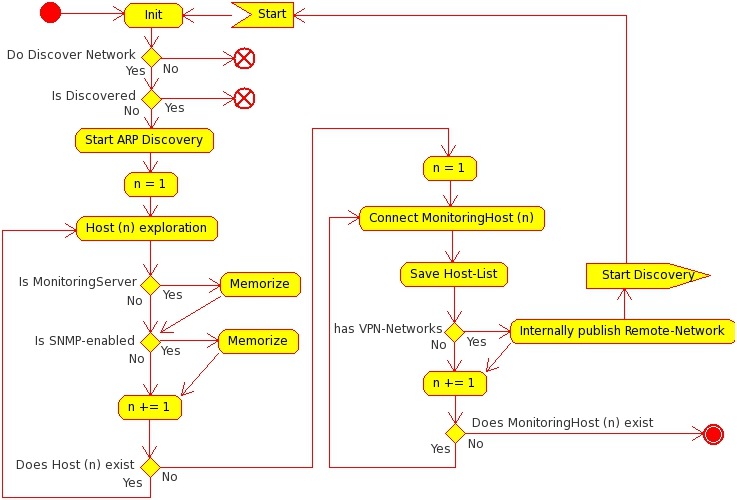
\includegraphics[width=\linewidth]{images/theorie/AutoDiscovery}
  \caption[Ablauf zum Suchen von neuen Systemen in einem Netzwerk]{Automatische Suche nach allen Hosts im internen wie auch in entfernten Netzwerken. Dieses wird nur neu ausgelesen, sofern dies nicht schon gemacht worden ist. Dadurch wird verhindert, dass ein Netzwerk von mehreren \"Uberwachungsservern nacheinander oder gleichzeitig ausgelesen wird.}
  \label{fig:discovery-ablauf}
\end{figure}


\subsection{Fazit: Problemfall Ger\"ateerkennung} \label{sec:theorie-discovery-fazit}
In gr\"osseren Netzwerken oder Verb\"unden verschiedener Netzwerke ist eine reine manuelle Konfiguration sehr aufw\"andig und daher praktisch unm\"oglich. Eine reine automatische Erkennung von Ger\"aten bietet jedoch eine zu geringe M\"oglichkeit zur individuellen Konfiguration der einzelnen Systeme.

Eine Mischform aus einer manuellen und einer automatischen Konfiguration ist die einfachste und komfortabelste L\"osung zur Einrichtung eines \"Uberwachungsnetzwerkes. Dabei k\"onnen einzelne Systeme jederzeit manuell in ein Netzwerk eingebunden, umkonfiguriert und ausgeschlossen werden, jedoch kann in einem Netzwerk auch automatisch nach neuen Komponenten gesucht werden.

Das zu implementierende System muss also \"uber beide M\"oglichkeiten verf\"ugen. Zum einen k\"onnen die \"Uberwachungsserver sowie verschiedene Komponenten in einem Netzwerk manuell konfiguriert werden, jedoch besteht auch die M\"oglichkeit dieses automatisch zu untersuchen. Dabei muss auf den \"Uberwachungsservern manuell definiert werden, welche Netzwerke miteinander verbunden sind und welche von diesen automatisch untersucht werden sollen, respektive welche nicht\footnote{\label{foot:theorie-discovery-fazit}Der Ausschluss eines Netzwerkes macht zum Beispiel bei Root-Servern Sinn, welche bei einem Hoster direkt im Internet sind, dort jedoch nicht das komplette Netzwerk, sondern nur eben der eine (oder mehrere) Server \"uberwacht werden soll.}. Diese Konfiguration muss nicht auf jedem \"Uberwachungsserver in jedem Netzwerk gemacht werden. Es reicht dabei aus, wenn diese Konfiguration auf einem einzelnen Server gemacht wird, denn die Konfiguration wird automatisch auf alle bekannten \"Uberwachungsserver \"ubertragen (siehe \ref{sec:theorie-config-fazit}).


%%%%%%%%%%%%%%%%%%%%%%%%%%%%%%%%%%%%%%%%%%%%%%%%%%%%%%%%%%%%%%%%%%%%%%%%%%%%%%%%%%%%%%%%%%%%%%%%%%%%%%%%%%%%%%%%%%%%%%%%%%%%%%%%%%%%%%%%%
\section{Problemfall Konfiguration} \label{sec:theorie-config}
Die verschiedenen \"Uberwachungsserver k\"onnen, wie zum Beispiel unter \ref{sec:theorie-discovery-fazit} definiert, unterschiedlich und individuell konfiguriert werden. Das gesamte \"Uberwachungsnetzwerk kann also auf jedem X-Beliebigen \"Uberwachungsserver ver\"andert werden. Diese Konfiguration muss anschliessend nicht nur auf alle anderen Systeme \"ubertragen sondern auch abgeglichen werden.

\subsection{M\"oglichkeiten zur Konfigurationsspeicherung} \label{sec:theorie-config-variants}
Grunds\"atzlich kann zwischen einer globalen und einer individuellen Konfiguration unterschieden werden.

\subsubsection{Global zusammengefasste Konfiguration} \label{sec:theorie-config-variants-global}
Eine M\"oglichkeit besteht darin, dass jeder \"Uberwachungsserver jeweils die komplette Konfiguration speichert.

Der Vorteil bei dieser Art der Speicherung liegt in der einfachen Handhabung, denn es gibt nur eine einzige Konfiguration. Diese kann auf einem beliebigen System angepasst und anschliessend 1:1 an alle anderen Server wieder ausgeliefert werden.

Nachteilig an dieser Variante ist jedoch, dass bei einem grossen \"Uberwachungsnetzwerk die Konfiguration relativ gross werden kann. Je nach Anzahl Komponenten und Diensten wird diese Art der Konfiguration relativ schnell komplex und wahrscheinlich fast nicht mehr \"uberschaubar (ohne entsprechende Konfigurations-Hilfen/-Programme).

\subsubsection{Individuelle Konfiguration} \label{sec:theorie-config-variants-individual}
Die zweite M\"oglichkeit beinhaltet eine individuelle Konfiguration auf jedem einzelnen System. Jeder \"Uberwachungsserver besitzt somit nur seine jeweilige Konfiguration und weiss dadurch auch nur, was er zu \"uberwachen hat. Die restlichen Systeme und Netzwerke sind ihm nicht bekannt.

Der Vorteil dieser Variante liegt eindeutig in der Konfigurationsgr\"osse, welche relativ klein und pro System sehr \"ubersichtlich ist.

Der grosse Nachteil liegt im Management der verschiedenen Konfigurationen. F\"ur einen globalen \"Uberblick \"uber die komplette Konfiguration, oder auch nur dar\"uber, welche Server den einen Dienst auf einem Server \"uberwacht, muss die komplette Konfiguration aus dem ganzen \"Uberwachungsnetzwerk zusammengesucht, kombiniert und ausgewertet werden. F\"ur diesen Vorgang m\"ussen nicht nur alle \"Uberwachungsserver im eigenen Netzwerk bekannt sein und abgefragt werden sondern auch alle in allen anderen Netzwerken.

\subsection{Fazit: Problemfall Konfiguration} \label{sec:theorie-config-fazit}
Das zu entwickelnde \"Uberwachungssystem soll sich automatisch, autonom und vor allem hochverf\"ugbar \"uberwachen. Eine Voraussetzung ist somit, eine schnelle und vor allem unkomplizierte Auswahl von verschiedenen \"Uberwachungspartnern. Dies kann nur mit einer global zusammengefassten Konfiguration erreicht werden.

Die Performance der einzelnen Systeme ist auch eine Voraussetzung, gerade im Bereich der Hochverf\"ugbarkeit. Dieser Aspekt kann jedoch nur durch eine individuelle lokale Konfiguration gew\"ahrleistet werden.

Durch diese Voraussetzungen kommt nur eine Kombination der beiden Varianten in Frage. Zus\"atzlich wird die Konfiguration noch in verschiedene Bereiche aufgeteilt, welche separiert gespeichert und abgefragt werden k\"onnen.

\subsubsection{Konfiguration der Netzwerke} \label{sec:theorie-config-fazit-network}
Die verschiedenen Netzwerke sowie die Verbindungen zwischen diesen werden in einer globalen, netzwerk\"ubergreifenden Konfiguration gespeichert. Dadurch wissen immer alle \"Uberwachungssysteme, welche anderen Netzwerke \"uberwacht werden und wie auf diese zugegriffen wird. Diese Konfiguration beinhaltet nur die Netzwerke und deren Daten zur Fragmentierung, Angaben ob das Netzwerk automatisch untersucht werden darf (siehe \ref{sec:theorie-discovery-fazit}), Verbindungsdaten f\"ur die Verbindungen (siehe \ref{sec:theorie-nat-fazit}) sowie eventuelle weitere Daten, welche auf den Netzwerken definiert werden m\"ussen. Dies k\"onnen zum Beispiel Dienste sein, welche von ausserhalb erreichbar sein m\"ussen, etc.

Diese globale Konfiguration ist nicht als eine zentrale Datenbank zu sehen sondern als eine Konfiguration, welche auf jedem System gleich ist. Bei einer Anpassung wird somit jedes System mit der neuen Konfiguration versehen und nicht nur das betroffene System.

\subsubsection{Konfiguration der Hosts und Systeme} \label{sec:theorie-config-fazit-systems}
Die verf\"ugbaren Hosts sowie deren Dienste, die \"uberwacht werden sollen, sind jeweils nur Netzwerkintern als globale Konfiguration vorhanden. Diese Konfiguration wird jeweils bei einer automatischen Ger\"ateerkennung und auch einer manuellen Anpassung neu geschrieben und verteilt. Auch diese globale Konfiguration ist nicht eine zentrale Datenbank, sondern grunds\"atzlich einfach auf jedem System gleich.

Interne Dienste, wie beispielsweise die \"Uberwachung des Arbeitsspeichers oder der Systemlast, werden gleich behandelt wie externe Dienste. Alle internen Dienste sollten ebenfalls \"uber einen SNMP-Dienst von extern abrufbar sein.

Durch diese Konfiguration weiss jedes System, was auf welchem anderen System laufen muss, was f\"ur Probleme auftreten k\"onnen und was bei einem Fehler passieren soll.

\subsubsection{Konfiguration der \"Uberwachungspartner} \label{sec:theorie-config-fazit-partner}
Die Auswahl der \"Uberwachungspartner muss automatisch und autonom erfolgen (siehe \ref{sec:theorie-fragmentierung}). Die Konfiguration, welches System welche Hosts und Dienste \"uberwacht, wird jeweils auf den Systemen und nicht global gespeichert. Somit kann schnell eruiert werden, wann was wo \"uberwacht werden soll, ohne zuerst andere Systeme an zu fragen, ob dies noch der Fall ist oder ob sich etwas ge\"andert hat.

Diese Konfiguration wird automatisch erstellt, gewartet und gel\"oscht. Sie kann nicht manuell bearbeitet werden.


%%%%%%%%%%%%%%%%%%%%%%%%%%%%%%%%%%%%%%%%%%%%%%%%%%%%%%%%%%%%%%%%%%%%%%%%%%%%%%%%%%%%%%%%%%%%%%%%%%%%%%%%%%%%%%%%%%%%%%%%%%%%%%%%%%%%%%%%%
\section{Problemfall Host-Fragmentierung} \label{sec:theorie-fragmentierung}
Sind alle Systeme gefunden und untersucht, muss in einem n\"achsten Schritt festgelegt werden, welche \"Uberwachungsserver welche anderen Systeme \"uberwachen sollen.

Die Grundfrage "`Wer \"uberwacht wen?"' beinhaltet folgende weiteren Fragestellungen, welche bei den verschiedenen Methoden zur Hostfragmentierung gekl\"art werden m\"ussen:
\begin{itemize}
 \item Werden die Dienste nur Netzwerk intern \"uberwacht oder auch von externen Systemen?
 \item Wie viele Server \"uberwachen einen einzelnen Dienst auf einem System?
 \item K\"onnen verschiedene \"Uberwachungen zu unterschiedlichen Zeitpunkten gemacht werden?
 \item Darf ein Server denjenigen \"uberwachen, welcher einen seiner Dienste \"uberwacht?
 \item \"Uberwacht ein Server nur einen einzelnen Server oder \"uberwacht er verschiedene Systeme?
 \item \"Uberwacht ein Server alle Dienste eines anderen oder nur einzelne?
\end{itemize}

In Kapitel \ref{sec:theorie-nat-fazit} wurde die Verbindung zwischen unterschiedlichen Netzwerken behandelt. Dadurch ist die erste Frage schon abgehandelt. In jedem Netzwerk steht mindestens ein \"Uberwachungsserver, welcher eine Verbindung in die anderen Netzwerke hat. Diese Server sind daf\"ur zust\"andig, die entfernten Netzwerke zu \"uberwachen. Das beinhaltet nicht nur die Erreichbarkeit, sondern auch die \"Uberwachung aller Dienste, welche als "`von extern zu \"uberwachen"' konfiguriert worden sind (siehe Kapitel \ref{sec:theorie-config-fazit-network}).

Die Frage nach der Anzahl Server, welche einen einzelnen Dienst auf einem System \"uberwachen, kann einfach beantwortet werden: Durch die Definition einer hochverf\"ugbaren \"Uberwachung, sollte ein Dienst, wenn m\"oglich, immer von mehreren anderen Systemen \"uberwacht werden und nicht nur von einem einzelnen. F\"allt ein System aus, wird die \"Uberwachung somit immer noch von mindestens einem anderen Ger\"at durchgef\"uhrt.

Die restlichen Fragen gehen in den Bereich der Performance und der Lastverteilung.

\subsection{Lastverteilung} \label{sec:theorie-frag-last}
Die Systemlast sollte, gerade da es sich um eine hochverf\"ugbare \"Uberwachung handelt und die Server nicht zus\"atzlich belastet werden sollen, m\"oglichst gering sein und somit eine hohe Performance aufweisen. Die zu \"uberwachenden Dienste m\"ussen also m\"oglichst gleichverteilt auf alle internen \"Uberwachungsserver verteilt werden. Durch diese Gleichverteilung kann davon ausgegangen werden, dass jeder \"Uberwachungsserver eine \"ahnliche, zus\"atzliche Grundlast aufweist. Mit der Formel
\begin{equation}
 L = {X \times N}
\label{eq:theorie-frag-nonshared}
\end{equation}
kann berechnet werden, was f\"ur eine zus\"atzliche Last $L$ ein \"Uberwachungsserver verkraften muss, wenn je nur ein einzelner Dienst von allen Servern \"uberwacht wird. Dabei wird f\"ur $X$ die Last des jeweiligen Dienstes und f\"ur $N$ die Anzahl \"uberwachter Server genommen.

\begin{table}[ht]
 \centering
 \begin{tabular}{r|c|c|c|c}
   & HTTP (50) & SMTP(10) & ICMP (5) & POP3 (30) \\
  \hline
  Server A & x & x & x & x \\
  \hline
  Server B & x &   & x &   \\
  \hline
  Server C &   &   & x &   \\
  \hline
  Server D & x & x & x & x \\
  \hline
  Server E & x &   & x &   \\
  \hline
  Total    & 4 & 2 & 5 & 2
 \end{tabular}
 \caption[Zu \"uberwachende Server und Dienste]{Beispiel: Verschiedene Server mit unterschiedlichen Diensten, die \"uberwacht werden sollen. In Klammern ein Dummy-Wert zur Berechnung, welcher die zus\"atzliche "`Last"' einer \"Uberwachung angibt. Eine HTTP-Dienst\"uberwachung mit Result-Auswertung braucht mehr Resourcen als eine einfacher ICMP-EchoRequest.}
 \label{tbl:theorie-frag-hosts}
\end{table}

\begin{table}[ht]
 \centering
 \begin{tabular}{r|c|c|c|c|c}
   & HTTP (50) & SMTP(10) & ICMP (5) & POP3 (30) & Zus\"atzliche Last \\
  \hline
  Server A & 4 &   &   &   & 200 \\
  \hline
  Server B &   & 2 &   &   & 20 \\
  \hline
  Server C &   &   & 5 &   & 25 \\
  \hline
  Server D &   &   &   & 2 & 60 \\
  \hline
  Server E &   &   &   &   & 0
 \end{tabular}
 \caption[Lastenvergleich, wenn gruppiert nach Dienst \"uberwacht wird]{Beispiel: Jeder Server \"ubernimmt die \"Uberwachung von einem einzelnen Dienst. In Klammern ein Dummy-Wert zur Berechnung, welcher die zus\"atzliche "`Last"' einer \"Uberwachung angibt. Jeder Server hat somit eine stark unterschiedliche Zusatzlast, mit Ausnahme von Server E, welcher nicht weiter belastet wird. Problematisch sind nicht nur die unterschidlichen Lasten, sondern auch dass die Server ihre eigenen Dienste \"uberwachen m\"ussen.}
 \label{tbl:theorie-frag-nonshared}
\end{table}

Damit die zus\"atzliche Grundlast m\"oglichst gleichverteilt auf allen Systemen ist, sollte eine m\"oglichst gemischte Dienst\"uberwachung gew\"ahlt werden. Die verschiedenen Dienst\"uberwachungen weisen wahrscheinlich unterschiedliche Lasten in der Verarbeitung auf, denn bei den einen Diensten muss lediglich die Erreichbarkeit gekl\"art werden, bei anderen m\"ussen eventuell komplexe Stringmanipulationen oder verschiedene Sende- und Empfangs-Aktionen durchgef\"uhrt werden. Durch die Definition, dass ein \"Uberwachungsserver unterschiedliche Dienste \"uberwacht, kann also sichergestellt werden, dass eine Lastverteilung stattfindet. Mit der Formel
\begin{equation}
 L = \sum_{i=0}^{N} {X_i}
\label{eq:theorie-frag-shared}
\end{equation}
kann diese Zusatzlast $L$, welche ein Server verkraften muss, berechnet werden. Dabei ist $i$ ein Z\"ahler von $0$ bis zur Anzahl Dienste $N$ und $X_i$ die jeweilige Last des aktuellen Dienstes.

F\"ur eine genaue Berechnung und optimale Lastverteilung ist es dabei notwendig, dass die Summe der Last der Dienste gleichm\"assig auf alle Server verteilt werden kann. Es m\"usste also "`$AnzahlDienste \mod AnzahlServer = 0$"' gegeben sein, um eine optimale Verteilung zu gew\"ahrleisten. Diese Definition sagt aus, dass jedem Server gleich viele Dienste zugewiesen werden k\"onnen, die Berechnung $AnzahlDienste \over AnzahlServer$ also keinen Rest ergibt - Wobei bei dieser Definition die Last der Dienste nicht beachtet wird. Ein Vergleich zwischen den zwei Varianten ist, basierend auf den Daten aus Tabelle \ref{tbl:theorie-frag-hosts}, in den Tabellen \ref{tbl:theorie-frag-nonshared} und \ref{tbl:theorie-frag-shared} zu sehen.

\begin{table}[ht]
 \centering
 \begin{tabular}{r|c|c|c|c|c}
   & HTTP (50) & SMTP(10) & ICMP (5) & POP3 (30) & Zus\"atzliche Last \\
  \hline
  Server A & 1 &   & 1 &   & 55 \\
  \hline
  Server B & 1 & 1 & 1 &   & 65 \\
  \hline
  Server C & 1 &   & 1 & 1 & 85 \\
  \hline
  Server D & 1 &   & 1 &   & 55 \\
  \hline
  Server E &   & 1 & 1 & 1 & 45
 \end{tabular}
 \caption[Lastenvergleich, wenn die Dienste auf alle Server aufgeteilt werden]{Beispiel: Die 13 Dienste werden auf die verschiedenen Server aufgeteilt. Somit werden die Lasten nahezu gleich auf alle Server verteilt.\newline}
 \label{tbl:theorie-frag-shared}
\end{table}

Eine andere M\"oglichkeit besteht darin, dass ein \"Uberwachungsserver jeweils alle Dienste von einem oder von mehreren anderen Systemen \"uberwacht. Die dabei anfallende Last kann mit der Formel
\begin{equation}
L = \sum_{k=0}^{M} \left( \sum_{i=0}^{N} {X_{k_i}} \right)
\label{eq:theorie-frag-sysshared}
\end{equation}
berechnet werden, wobei $M$ die Anzahl der Server, $N$ die Anzahl der Dienste auf dem Server $M_k$ und $X_{k_i}$ die Last des Dienstes $X_i$ auf dem aktuellen Server ist. Tabelle \ref{tbl:theorie-frag-sysshared} zeigt die Systemlasten, welche bei einer solchen \"Uberwachung anfallen w\"urden.

\begin{table}[ht]
 \centering
 \begin{tabular}{r|c|c|c|c|c}
   & HTTP (50) & SMTP(10) & ICMP (5) & POP3 (30) & Total Last \\
  \hline
  Server A & 1 & 1 & 1 & 1 & 95 \\
  \hline
  Server B & 1 &   & 1 &   & 55 \\
  \hline
  Server C &   &   & 1 &   & 5 \\
  \hline
  Server D & 1 & 1 & 1 & 1 & 95 \\
  \hline
  Server E & 1 &   & 1 &   & 55
 \end{tabular}
 \caption[Lastenvergleich, wenn alle Dienste eines Servers \"uberwacht werden]{Beispiel: Alle Dienste auf einem System werden von einem Server \"uberwacht. Die Tabelle zeigt die Lasten, welche beim \"Uberwachungs-Server anfallen w\"urden.}
 \label{tbl:theorie-frag-sysshared}
\end{table}

Da ein System meistens mehrere andere Rechner \"uberwacht, muss bei dieser Variante darauf geachtet werden, dass die Auswahl der unterschiedlichen Systeme zu einer gleichverteilten Last f\"uhrt. Die zus\"atzliche Last sollte also bei jedem \"Uberwachungsserver um den Mittelwert aller Lasten liegen. Um dies zu erreichen, kann ein einfacher Algorithmus (siehe Codeblock \ref{alg:theorie-frag-mittelwert}) angewendet werden.
\begin{figure}[H]
 \lstset{language=Pascal}
 \begin{lstlisting}[mathescape,literate={<=}{{$\leq$}}1{>=}{{$\geq$}}1{<>}{{$\neq$}}1,label=alg:theorie-frag-mittelwert,caption={[Gleicheverteile Lastenverteilung der Dienste auf Server]Mit diesem Algorithmus werden alle zu \"uberwachenden Dienste und Server gleichverteilt auf alle \"Uberwachungsserver verteilt. Die Server liegen dabei als Liste $hosts \Rightarrow [h_1, h_2, ..., h_k]$ vor. Die Hosts werden der Last nach sortiert und anschliessend immer die beiden \"aussersten Systeme (also der Last-Intensivste und -Extensivste) einem Host zugewiesen.}]
if numMonitor >= 1 and numMonitor <= length(hosts)-1 then
  result {}
end

if count(hosts) = 2 then
  result { $h_1$:[$h_2$], $h_2$:[$h_1$] }
end

back = {}
intensiveLoad = floor(numMonitor / 2)
extensiveLoad = intensiveLoad

if numMonitor modulo 2 <> 0 then
  extensiveLoad = intensiveLoad + 1
end

hosts = sort_ascending_by_load(hosts)
monitoredHosts = []

for host in hosts do
  if length(monitoredHosts) = length(hosts) then
    monitoredHosts = []
  end

  x = 0
  while length(back[host]) <> intensiveLoad do
    if length(monitoredHosts) = length(hosts) break
    if hosts[x] <> host and hosts[x] not in monitoredHosts then
      add hosts[x] to back[host]
      add hosts[x] to monitoredHosts
    end
    x += 1
  end

  x = length(hosts) - 1
  while length(back[host]) <> intensiveLoad + extensiveLoad do
    if length(monitoredHosts) = length(hosts) break
    if hosts[x] <> host and hosts[x] not in monitoredHosts then
      add hosts[x] to back[host]
      add hosts[x] to monitoredHosts
    end
    x -= 1
  end
end

result back
 \end{lstlisting}
\end{figure}


\subsection{Anzahl \"Uberwachungspartner} \label{sec:theorie-fragmentierung-numhosts}
Durch die Anzahl der \"Uberwachungspartner wird nicht nur die Grundlast, welche auf den Servern anf\"allt, definiert, sondern auch die zus\"atzliche Last im Netzwerk, sowie der gesamte Vernetzungsplan. Durch die definierte Autonomit\"at der \"Uberwachungsstrategie, sollte also nicht eine fixe Anzahl an Verbindungen vorgegeben werden, sondern diese sollte automatisch berechnet werden.

Eine M\"oglichkeit best\"unde darin, dass einfach jeder Rechner jeden anderen \"uberwachen w\"urde. Dies w\"are jedoch nicht nur performancetechnisch Unsinn, sondern auch administrativ. F\"allt beispielsweise in einem Netzwerk mit 100 Rechnern ein System aus, w\"urden 99 andere Systeme das bemerken und m\"ussten untereinander ausmachen, wer denn nun den Alert ausl\"ost und versendet.

Es muss also ein Algorithmus entworfen/gefunden werden, welcher die ideale Anzahl an Verbindungen zwischen verschiedenen Knotenpunkten herstellt. Die Distanz zwischen zwei Punkten, respektive zwischen zwei Systemen kann dabei vernachl\"assigt werden, denn die Latenzen in einem internen Netzwerk m\"ussen sowieso als sehr klein angenommen werden\footnote{\label{foot:theorie-frag-latenzen}Sind die Latenzen in einem internen Netzwerk, also z.B. einem Geb\"aude, schlecht, stimmt entweder etwas an der Verkabelung nicht, das Netzwerk ist \"uberlastet oder es werden alte Komponenten eingesetzt, welche mit der Last nicht zurecht kommen.}.

In der Informatik schon lange eingesetzte und bew\"ahrte Techniken bei Kommunikationsintensiven Abl\"aufen sind die Hypercube-Algorithmen\footnote{Danke an dieser Stelle f\"ur den Hinweis auf die Hypercubes an Herr Dr. Frank Moehle.}. Die nachfolgenden Formeln sowie die Definitionen der Hamming-Distanz sind in vielen Fachliteraturen und im Internet verf\"ugbar, zum Beispiel im Dokument von Hans Walser: Der n-dimensionale Hyperw\"urfel \cite{hypercube}. Dieses Dokument diente als Grundlage f\"ur den Aufbau des grundlegenden Verst\"andnisses der Hyperw\"urfel.

Ein Hypercube, auch Hyperw\"urfel genannt, stellt grunds\"atzlich ein Netzwerk aus Knoten und Verbindungen dar (siehe Abbildung \ref{fig:hyper-sample} im Anhang). Der Einsatz der Hypercubes im Bereich des Hypercomputing oder auch Clustering r\"uhrt daher, dass grunds\"atzlich von jedem Knoten des Hypercubes eine Verbindung zu jedem anderen Knoten besteht. Die Anzahl an Verbindungen bleibt dabei jedoch \"uberschaubar, da nicht einfach jeder Knoten mit jedem anderen verbunden wird. Es bestehen aber auch nicht zu wenige Verbindungen, so dass das Fehlen eines Systems nicht zu einem Totalausfall f\"uhrt.

Bei einem Hypercube werden alle Systeme je einem Knoten zugewiesen. Die Distanz zwischen zwei Systemen ist im Optimalfall $1$, im schlimmsten Fall gleich der Dimension $n$ des Hypercubes\footnote{\label{foot:hypercube-dimension}Die Dimension beim Hypercube ergibt sich aus der Anzahl von Systemen, die \"uberwacht werden m\"ussen siehe Abbildung \ref{fig:hyper-sample} im Anhang}. Diese Distanz wird auch \textit{Hamming-Distanz}\footnote{\label{foot:hypercube-hamming}Die \textit{Hamming-Distanz} findet ihren Ursprung bei Richard Wesley Hamming, welcher durch den Hamming-Code eine Selbst-Korrigierende \"Ubermittlungsmethode entwickelte.} genannt, entsprechend werden im Hypercube auch die verschiedenen Ecken nummeriert und verbunden (siehe Abbildung \ref{fig:hyper-hamming-num} im Anhang).

Zur Bestimmung der Dimension des Hypercubes muss die Anzahl der Systeme bekannt sein. Die Anzahl Ecken in einem Hypercube wird definiert durch $2^n$, wobei $n$ die Dimension ist. Es muss also die n\"achst h\"ohere Zweierpotenz gefunden werden, um die Dimension des Hypercubes zu bestimmen (siehe Codeblock \ref{alg:theorie-hypercube-dimension}). Basierend auf der Dimension k\"onnen anschliessend alle weiteren Daten berechnet werden.

\begin{figure}[H]
 \lstset{language=[ANSI]C}
 \begin{lstlisting}[label=alg:theorie-hypercube-dimension,caption={[N\"achst h\"ohere Zweierpotenz finden]Algorithmus zum Auffinden der n\"achst h\"oheren Zweierpotenz zur Dimensionsbestimmung eines Hypercubes anhand der Anzahl Systeme. Die Schlaufe "`schiebt"' dabei die 1 in der bin\"aren Darstellung so lange nach links bis die Potenz gr\"osser oder gleich der Anzahl Systeme ist.}]
// bin: 0000 0001
power = 1
if (numHosts > 1) {
  while (power < numHosts) {
    // Shift left as long as power is less than numHosts
    // bin: 0000 0010, 0000 0100, 0000 1000, ...
    power <<= 1
  }
}
return power
 \end{lstlisting}
\end{figure}

Die Anzahl \"Uberwachungspartner bei einem Hypercube ist immer gleich der Dimension. Somit kann durch den Algorithmus in Codeblock \ref{alg:theorie-frag-mittelwert} bestimmt werden, welche Systeme welche anderen \"uberwachen. Dies jedoch nur unter der Voraussetzung, dass jedes System das \"uberwacht wird, ebenfalls ein \"Uberwachungsserver ist. Das kann aber nicht als Voraussetzung gegeben werden, denn in einem Netzwerk werden oft Ger\"ate eingesetzt, welche sich zwar \"uberwachen lassen, selber jedoch nicht in der Lage sind, andere Systeme zu \"uberwachen - geschweige denn es zulassen, Software nach zu installieren, welche diese Funktionalit\"at \"ubernehmen w\"urde.

Eine M\"oglichkeit, dieses Problem zu umgehen w\"are, eine spezielle Anordnung der Nodes im Hypercube. Dies w\"urde eine relative Verkomplizierung des Algorithmus nach sich ziehen, denn bei jeder Platzierung m\"ussten alle Nachbarknoten angeschaut werden und auf die \"Uberwachungsf\"ahigkeit untersucht werden.

Eine weitaus einfachere M\"oglichkeit ist, den Hypercube nur mit den \"Uberwachungsservern als Knoten zu erstellen. Die restlichen Systeme werden anschliessend einfach harmonisch auf alle \"Uberwachungsserver aufgeteilt.

Durch folgende Vorgehensweise kann schnell und einfach eine \"Uberwachung basierend auf einem Hypercube aufgebaut werden:
\begin{enumerate}
 \item Dimension des Hypercubes anhand aller \"Uberwachungsserver feststellen
 \item Hypercube mit allen \"Uberwachungsservern erstellen
 \item \"Uberwachungspartner festlegen, die Anzahl ist gleich der Dimension
 \item Die restlichen Systeme auf alle \"Uberwachungsserver aufteilen
\end{enumerate}

\subsection{Leere Knoten im Hypercube} \label{sec:theorie-fragmentierung-spof}
Die Vernetzung aller \"Uberwachungsserver mittels einem Hypercube ist eine schnelle und nicht sehr rechenintensive Angelegenheit. Ein Hypercube, welcher basierend auf einer Anzahl Hosts aufgebaut wird, welche keine Zweierpotenz ist, weist aber eine grosse Unsch\"onheit auf: leere Knoten. Gerade wenn ein Hypercube mit vielen Systemen erstellt wird, nimmt die Wahrscheinlichkeit zu, dass leere Knoten in einem Hypercube vorhanden sind.

Im schlimmsten Fall kann ein Node durch diese leeren Knoten so abgeschirmt werden, dass dieser nur Verbindungen zu leeren Knoten aufweist. Eine Illustrierung dieses Problems wird in Abbildung \ref{fig:hyper-spof-9hosts} gezeigt. Ein Hypercube, der basierend auf 9 Systemen aufgebaut wird, muss in der Dimension $d=4$ erstellt werden. Das bedeutet, dass es total $2^4 - 9 = 16 - 9 = 7$ leere Knoten gibt und jeder Knoten 4 Verbindungen aufweist. Im extremsten Fall k\"onnen so bis zu vier Nodes komplett abgeschirmt sein. Bei einer Verwendung des Hypercubes zur Gew\"ahrleistung von Verbindungen von jedem Node im Netzwerk zu jedem anderen, kann dies zu schwerwiegenden Problemen f\"uhren.

\begin{figure}[ht]
  \centering
  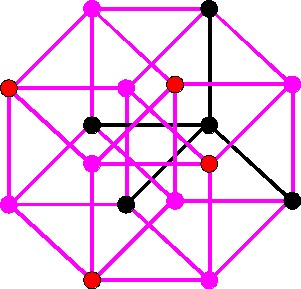
\includegraphics[width=0.5\linewidth]{images/theorie/hyper-spof-9hosts}
  \caption[Ein Hypercube der vierten Dimension]{Ein Hypercube der vierten Dimension mit 9 Hosts (schwarz, rot) weist 7 leere Knoten auf (magenta). Bei einer ungl\"ucklichen Zuweisung der Nodes k\"onnen so bis zu vier Systeme ohne Verbindung sein (rot).}
  \label{fig:hyper-spof-9hosts}
\end{figure}

Beim Aufbauen eines Hypercubes muss also immer darauf geachtet werden, dass die Nodes nicht willk\"urlich im Hypercube verteilt werden, sondern dass diese der Reihe nach aufgef\"ullt werden. Dadurch kann gew\"ahrleistet werden, dass jeder Knoten mindestens eine Verbindung aufweist.



%%%%%%%%%%%%%%%%%%%%%%%%%%%%%%%%%%%%%%%%%%%%%%%%%%%%%%%%%%%%%%%%%%%%%%%%%%%%%%%%%%%%%%%%%%%%%%%%%%%%%%%%%%%%%%%%%%%%%%%%%%%%%%%%%%%%%%%%%
\section{Problemfall ALERT-\"Ubermittlung} \label{sec:theorie-alert}
Wird von einem System ein Fehler entdeckt, muss dies je nach Konfiguration einer entsprechenden Person oder Stelle gemeldet werden. Die Problematik liegt nun darin, dass ein System, respektive Dienst, von mehreren anderen Systemen zu unterschiedlichen Zeitpunkten \"uberwacht wird. Eine Meldung sollte aber wenn m\"oglich nur einmal versendet werden und nicht von jedem \"Uberwachungssystem aus, welches den Fehler bemerkt.

\subsection{Zentrale Meldestelle} \label{sec:theorie-alert-zentral}
Eine M\"oglichkeit diese mehrfache Alert-Auslieferung in den Griff zu bekommen, w\"are eine zentrale Meldestelle. Jedes Problem, welches entdeckt wird, wird umgehend dieser zentralen Stelle gemeldet. Eine Meldung muss dabei mindestens die Zeit der \"Uberwachung, den Meldungs-Typen sowie allf\"allige Daten beinhalten. In regelm\"assigen Abst\"anden werden alle gespeicherten und nicht versendeten Meldungen ausgelesen, gruppiert und verschickt.

Die Gruppierung der Meldungen nach dem Zeitrahmen und Meldungs-Typ hat den Hintergrund, dass die verschiedenen \"Uberwachungssysteme die Pr\"ufungen zwar nicht zum gleichen Zeitpunkt daf\"ur aber im gleichen Intervall\footnote{Ein System soll zum Beispiel alle 5 Sekunden mit einem ECHO-Request auf Anwesenheit gepr\"uft werden. Dieses Interval kann prinzipiell gew\"ahrleistet werden, nicht jedoch dass jedes System die gleiche Pr\"ufung in der gleichen (Nano/Mili)Sekunde ausf\"uhrt.} ausf\"uhren. Werden nun alle Nachrichten innerhalb eines solchen Intervalls ausgelesen (unter Beachtung des Systems und Dienstes), kann theoretisch ausgeschlossen werden, dass der gleiche Vorfall mehrfach gemeldet wird.

Der Vorteil einer solchen zentralen Instanz w\"are klar die einfache Bearbeitung aller Fehler. Der Nachteil liegt jedoch in der Definition und der Auslegung des gesamten \"Uberwachungs-Systems. Da das komplette System "`hochverf\"ugbar"' sein muss, w\"are eine einzelne wenn auch nur Netzwerk interne Alert-Instanz ein Widerspruch sowie eine Fehlerquelle. Funktioniert diese zentrale Instanz nicht oder ist diese nicht erreichbar, k\"onnen aus dem gesamten Netzwerk keine Fehler gemeldet werden.

\subsection{Hochverf\"ugbare Alert-\"Ubermittlung} \label{sec:theorie-alert-ha}
Um dem Paradigma der Hochverf\"ugbarkeit gerecht zu werden, sollte prinzipiell jeder \"Uberwachungsserver in der Lage sein, einen Fehler eigenst\"andig zu melden. In diesem Szenario gibt es zur Vermeidung von mehrfachen Meldungen grunds\"atzlich zwei M\"oglichkeiten\footnote{Diese zwei M\"oglichkeiten beschreiben die Basisfunktionalit\"at - Kombinationen und Verfeinerungen, etc. sind m\"oglich, werden aber nicht als weitere M\"oglichkeiten gelistet.}:

\begin{itemize}
 \item[POLL:] Wird ein Fehler entdeckt, m\"ussen alle anderen Systeme, welche das gleiche System und den gleichen Dienst \"uberwachen, angefragt werden, ob dieser Fehler innerhalb der letzten X Zeiteinheiten schon gemeldet worden ist. Ist dies nicht der Fall, wird eine Meldung gesendet und der Status gespeichert.
 \item[PUSH:] Wird ein Fehler entdeckt, m\"ussen alle anderen Systeme benachrichtigt werden, dass dieser Fehler zum Zeitpunkt X gemeldet worden ist. Entdeckt ein anderes System den gleichen Fehler, kann es durch diese interne Liste pr\"ufen, ob der gefundene Fehler innerhalb der letzten X Zeiteinheiten schon gemeldet worden ist oder nicht.
\end{itemize}

Bei beiden m\"oglichen Szenarien besteht die Gefahr, dass das Netzwerk unn\"otigerweise belastet respektive \"uberflutet wird. Jedes System setzt nach der offiziellen \"Uberwachung noch weitere Anfragen an alle anderen Systeme ab. Die Anzahl der Anfragen\footnote{Wenn $n$ Systeme gleichzeitig an alle $n-1$ anderen Systeme eine Anfrage stellen, sind gleichzeitig $n*(n-1)$ Requests auf dem Netzwerk} kann sich dadurch auf ein Maximum von $n*(n-1)$ kumulieren.

Die Anfragen und Antworten werden wahrscheinlich relativ kleine Datenpakete sein. Die heutigen internen Netzwerke sind rasend schnell, jedoch sollen mit der angestrebten L\"osung auch Systeme mit einer schwachen Leitung\footnote{Zum Beispiel ein einzelnes externes System, welches lediglich \"uber eine GSM-Verbindung verf\"ugt} und auch stark frequentierte und ausgelastete Netzwerke angesprochen und \"uberwacht werden k\"onnen. Bei der zu implementierenden L\"osung muss dieser Punkt unbedingt beachtet werden.

\subsection{Fazit: Problemfall ALERT-\"Ubermittlung} \label{sec:theorie-alert-fazit}
Das zu entwickelnde System muss hochverf\"ugbar sein, aus diesem Grund kommt eine zentrale Alert-Meldestelle, welche ausfallen k\"onnte, nicht in Frage. Jedes System muss in der Lage sein, eine Meldung zu versenden sowie eigenst\"andig zu eruieren, ob eine Meldung versendet werden soll und kann. Die einzelnen Systeme m\"ussen sich also gegenseitig sperren k\"onnen, was durch ein Mutex-Verfahren\footnote{Ein Mutex, englisch f\"ur \textbf{mut}ual \textbf{ex}clusion (wechselseitiger Ausschluss), verhindert, das nebenl\"aufige Prozesse oder Threads gleichzeitig auf gleiche Datenstrukturen zugreifen und diese ver\"andern.} realisiert wird. Ein einzelnes System muss also alle anderen Systeme mit einem \textit{Lock}\footnote{\textit{Locking} bedeutet \textit{Sperren}, also das beabsichtigte verhindern der Ausf\"uhrung einer Aktion, Funktion, Dateizugriff, etc.} versehen k\"onnen. Dabei wird basierend auf dem ausgefallenen Dienst, dem System und der Ausfallzeit auf jedem System ein \textit{Semaphor}\footnote{Ein Semaphor beschreibt in der Informatiok eine Datenstruktur zur Steuerung des ausschliessenden Zugriffes. Ein Semaphor beinhaltet alle Daten, welche genutzt werden, um den Ausf\"uhrungszeitpunkt zu bestimmen.} erstellt, welcher dieses Locking steuert. Durch die Zeit des Fehlers sowie eines konfigurierten Timeouts kann so jedes System feststellen, ob ein Fehler gemeldet werden soll oder nicht.

Ein m\"oglicher Ablauf einer \"Uberwachung und Alert-\"Ubermittlung ist in Abbildung \ref{fig:alert-sample} zu sehen. Bei dieser Visualisierung wird sowohl die PUSH- wie auch die POLL-Methode gezeigt. Bei einem POLL wird jedes mal beim Auftreten eines Fehlers jedes andere System angefragt, wann und ob der Fehler schon versandt worden ist. Jedes System gibt bei der Polling-Methode eine Semaphor zur\"uck, anhand welcher dies dann gepr\"uft werden kann. Rein rechnerisch kann die Anzahl Verbindungen, welche bei der POLL-Methode anfallen, durch
\begin{equation}
C = e \times (n-1)
\label{eq:theorie-alert-last}
\end{equation}
berechnet werden. Wobei $C$ die Anzahl an Verbindungen, $e$ die Anzahl der gleichen Fehler und $n$ die Anzahl Server beschreibt. Diese Formel kann auch f\"ur eine Standard-Implementation der PUSH-Methode verwendet werden, denn auch bei dieser muss bei jedem auftreten eines Fehlers eine Semaphor an jedes System gesendet werden.

\begin{figure}[h]
  \centering
  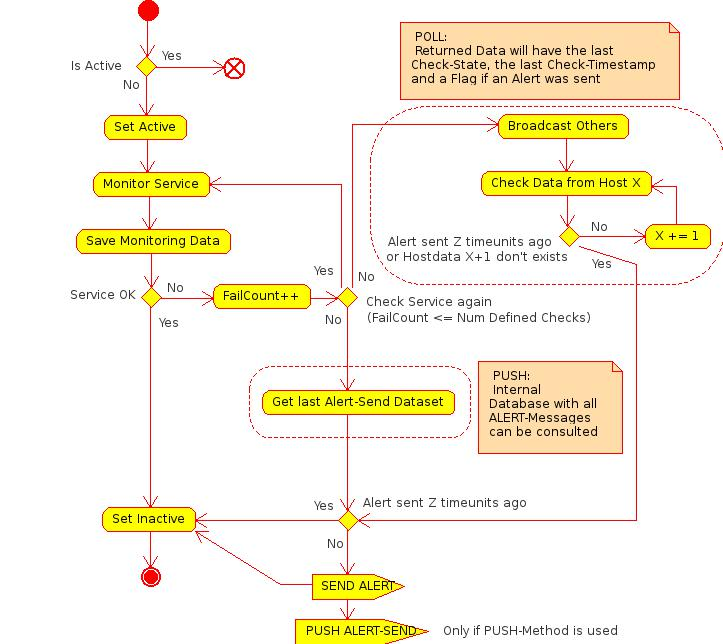
\includegraphics[width=0.9\linewidth]{images/theorie/AlertSend}
  \caption[Ablauf einer \"Uberwachung und Alarmmeldung]{Eine \"Uberwachung wird nur dann gestartet, wenn aktuell keine aktiv am laufen ist. Schl\"agt ein Test fehl, kann dieser erneut durchgef\"uhrt werden. Wenn alle Tests fehlgeschlagen sind, werden entweder alle anderen Systeme angefragt (POLL) und anhand deren Daten entschieden ob ein Meldung versendet werden muss oder nicht oder es werden die Internen Daten des letzten PUSH-Requests dazu verwendet.}
  \label{fig:alert-sample}
\end{figure}

Um die optimalste Anzahl an Verbindungen zu erlangen, muss die Anzahl an Fehlern $e$ in der obigen Formel \ref{eq:theorie-alert-last} reduziert oder gar weggelassen werden. Dieser Ansatz wurde in der PUSH-Methode in Abbildung \ref{fig:alert-sample} verwendet: Die Semaphor wird nur dann gesendet, wenn auch ein Alert verschickt wird. Das setzt voraus, dass jedes System alle Meldungen empf\"angt und intern speichert, denn nur so k\"onnen die Systeme die Semaphor f\"ur das Locking der Alerts nutzen. Semaphoren, welche durch die angegebene Zeiteinheit das Alerting nicht mehr blockieren, k\"onnen aus dem Speicher entfernt werden, so dass neue Fehler wieder gemeldet werden k\"onnen. Unter Ber\"ucksichtigung dieser Definition kann die Verbindungsanzahl durch \begin{equation}
C = (n-1)
\label{eq:theorie-alert-optimal}
\end{equation}
berechnet werden.

Ist ein System, durch einen Netzwerkausfall oder \"ahnliches, komplett isoliert\footnote{Ein System kann komplett isoliert sein durch fehlende oder falsche Routen, ausgesteckte oder defekte Netzwerkkabel, defekte Netzwerkkarten, uvm.} von allen anderen \"Uberwachungssystemen, kann ein Semaphor weder angefragt noch empfangen werden. Ist dies der Fall, und das Alerting ist nicht durch einen Lock gesperrt, wird der Fehler von dem System grunds\"atzlich gemeldet. In den meisten F\"allen f\"uhrt dies aber zu keinem doppelten oder mehrfachen Alert-Meldungs aufkommen, denn durch den Netzwerkfehler sind meistens auch die Alert-Nachrichten-Server (SMTP, SMS, etc.) nicht erreichbar. Durch die vernetzte Struktur wird das isolierte System aber von den anderen Servern erkannt und gemeldet.

Durch dieses Mutex-Verfahren kann bei den Alert-Meldungen komplett auf ein kompliziertes Transaktions-System verzichtet werden. Die Kombination des Push von Semaphoren und dem Locking reicht in den meisten F\"allen dazu aus, ein mehrfaches versenden von Alert-Meldungen zu unterbinden. Ausgeschlossen werden kann dies jedoch nicht, da der Empfangszeiptunkt der Semaphor nicht garantiert werden kann. Es besteht bei dieser Variante also die M\"oglichkeit, dass eine Semaphor zum Zeitpunkt $X$ gesendet und von einem System erst zum Zeitpunkt $X + 2$ empfangen wird. Pr\"uft nun das zweite System zum Zeitpunkt $X+1$ ob das senden erlaubt ist, weiss es nichts vom Sendeprozess des ersten Systems und sendet ebenfalls einen Alert. Durch eine Wartezeit zwischen dem Senden der Semaphore und dem Senden des Alerts sowie einer erneuten Pr\"ufen, kann dieses Problem umgangen werden. Wird bei der zweiten Pr\"ufung eine Semaphore gefunden, also ein Sendeprozess eines anderen Systems, erh\"allt jeweils das System mit dem kleineren Zeitstempel, also das erste System, den Vortritt zum Senden des Alerts.


%%%%%%%%%%%%%%%%%%%%%%%%%%%%%%%%%%%%%%%%%%%%%%%%%%%%%%%%%%%%%%%%%%%%%%%%%%%%%%%%%%%%%%%%%%%%%%%%%%%%%%%%%%%%%%%%%%%%%%%%%%%%%%%%%%%%%%%%%
\section{Techniken zur Nachrichten\"ubermittlung} \label{sec:theorie-msg}
Zur \"Ubermittlung von Nachrichten, sei dies durch einen Push- oder einen Pop-Request\footnote{\label{foot:push-pop}Ein Push-Request ist eine unaufgeforderte Zusendung von Daten; ein Pop-Request hingegen ist das aktive Anfragen von Daten}, gibt es nicht nur verschiedene Techniken sondern auch verschiedene Technologien. Zur \"Ubermittlung von \"Uberwachungsdaten haben sich dabei nachfolgende Standards etabliert, welche bei der zu implementierenden Software auch eingesetzt werden sollen.

\subsection{SNMP} \label{sec:theorie-snmp}
Das \textit{Simple Network Management Protocol} (SNMP) ist ein standardisiertes Netzwerkprotokoll zur \"Uberwachung und Steuerung von Netzwerkkomponenten. Das Protokoll wurde so festgelegt, dass prinzipiell jedes netzwerkf\"ahige Ger\"at in die \"Uberwachung aufgenommen werden kann. Dabei wird nicht nur der Aufbau der Datenpakete definiert, sondern ebenso der komplette Kommunikationsablauf. Um die Grundlast auf dem Netzwerk so gering wie m\"oglich zu halten, wird das Verbindungslose Protokoll UDP genutzt.

SNMP kennt insgesamt sechs verschiedene Paketarten. Die drei verschiedenen GET-Pakete\footnote{\label{foot:snmp-get-pkgs}SNMP kennt ein GET-Paket zum Anfragen von Daten, das GETNEXT-Paket um einen nachfolgenden Datensatz z.B. aus einer Tabelle aus zu lesen sowie das GETBULK-Paket zum Abrufen von mehreren Datens\"atzen} werden jeweils von einem Manager\footnote{Bei SNMP wird der Server mit Manager und der Client mit Agent beschrieben.} an einen Agenten gesendet, worauf dieser mit einem RESPONSE-Paket antwortet. Das SET-Paket wird genutzt um Parameter auf einem Agenten zu ver\"andern. Das TRAP-Paket schlussendlich ist ein einfacher Push-Request. Es wird also unaufgefordert ein Paket von einem Agenten an einen Manager gesendet. Traps werden dazu genutzt, um einen Manager dar\"uber zu informieren, dass ein Ereignis aufgetreten ist. Der Agent kann dabei nicht feststellen, ob das Paket beim Manager angekommen und verarbeitet worden ist, denn ein TRAP-Paket kann nicht durch ein RESPONSE-Paket best\"atigt werden.

SNMP definiert zwar den Aufbau der Datenpakete (siehe Anhang \ref{fig:snmp-packet}), nicht jedoch die Daten selbst, welche \"ubertragen werden. Die Daten und Werte, welche von einem Ger\"at ausgelesen werden k\"onnen, werden als "`Managed Object"' \"ubertragen. Diese MOs sind durch eine \texttt{Management Information Base} (MIB)\footnote{\label{foot:snmp-mib}Die MIB, definiert in RFC-1155\cite{rfc1155} (siehe auch RFC-4293\cite{rfc4293}, RFC-4022\cite{rfc4022}, RFC-4113\cite{rfc4113}), beinhaltet keine Daten sondern den Aufbau eines "`Managed Objects"', welches verwendet wird um Daten zu versenden/empfangen.} definiert. Die Basis jedes MIB ist der \texttt{Object Identifier} (OID)\footnote{\label{foot:snmp-oid}Eine OID sollte eine Weltweit eindeutige Identifikation sein, um Verwechslungen zu vermeiden. Firmen k\"onnen bei der IANA (Internet Assigned Numbers Authority, \url{http://www.iana.org/}) kostenlos eigene MIB-Module unterhalb "`iso.org.dod.internet.private.enterprise"' beantragen (\url{http://pen.iana.org/pen/PenApplication.page}). Unterhalb dieses Zweiges k\"onnen anschliessend eigene OIDs definiert werden.} sowie die Definition der unterschiedlichen Datenfelder. Diese Datenfelder weisen nicht nur einen Namen auf, sondern unterliegen auch einem Datentyp. Datentypen k\"onnen einfache Zahlen oder Texte sein, jedoch auch vordefinierte Muster wie zum Beispiel eine IPv4-Adresse (siehe Codeblock \ref{code:mib-ipAddress} im Anhang).

Aktuell sind verschiedene Versionen von SNMP verf\"ugbar und im Einsatz. SNMPv1 wurde 1988 definiert und setzte den Fokus nicht gross auf die Datensicherheit. Aus diesem Grund wurden verschiedene SNMPv2 Versionen definiert, welche alle unterschiedliche Sicherheits- und Datenkonzepte aufweisen. Die am meisten verwendete Version ist SNMPv2-community (SNMPv2c). Die Sicherheit basiert bei SNMPv2c auf so genannten "`Communities"', bei welchen definiert werden kann, dass z.B. bei \texttt{PUBLIC} nur gelesen, bei \texttt{PRIVATE} jedoch zus\"atzlich auch geschrieben werden darf. Eine Sicherheitsfunktion wie ein Passwort gibt es dabei nicht. Es kann zwar ein komplizierter Community-Name definiert werden, da SNMPv2c aber nicht verschl\"usselt wird, bringt auch das keinen wirklichen Schutz.

Die Versionen SNMPv1 bis SNMPv2c bieten also weder eine gute Verschl\"usselung noch eine sichere M\"oglichkeiten zur Authentifizierung. Aus diesem Grund wurde im Dezember 2002 die Spezifikation von SNMPv3\footnote{\label{foot:snmpv3-rfc}SNMPv3 wird in folgenden RFCs definiert: RFC-3410\cite{rfc3410}, RFC-3411\cite{rfc3411}, RFC-3412\cite{rfc3412}, RFC-3413\cite{rfc3413}, RFC-3414\cite{rfc3414}, RFC-3415\cite{rfc3415}, RFC-3416\cite{rfc3416}, RFC-3417\cite{rfc3417}, RFC-3418\cite{rfc3418}} ver\"offentlicht, welche Benutzer- und Ansichts basierende Zugriffsbeschr\"ankungen sowie andere Sicherheitsmechanismen beinhaltet. Gerade wegen diesen neuen Sicherheitsfunktionen, wie zum Beispiel der Schl\"usselverwaltung, ist SNMPv3 noch nicht sehr verbreitet.

\subsubsection{Fazit: SNMP} \label{sec:theorie-snmp-fazit}
Trotz gravierender sicherheits bezogener M\"angel der Versionen SNMPv1 bis SNMPv2c ist SNMP dennoch eine schnelle und einfache sowie gut erweiterbare Technologie zur Abfrage und \"Ubermittlung von einfachen Datens\"atzen. Sofern die Sicherheit keine grosse Rolle spielt, k\"onnen diese SNMP-Versionen ohne Bedenken eingesetzt werden. Zur \"Ubertragung von kritischen Daten muss entweder SNMPv3 in einer verschl\"usselten Variante oder SNMPv2c/SNMPv3 \"uber eine verschl\"usselte Verbindung respektive \"uber ein komplett abgeschirmtes Management-Netzwerk verwendet werden.

SNMP kann genutzt werden, wenn Daten von einem System auf ein anderes \"ubertragen werden sollen. So kann SNMP zum Beispiel gut f\"ur eine Leistungs\"uberwachung genutzt werden, nicht jedoch f\"ur die Funktionspr\"ufung eines Webservices oder anderen Dienstes wie SMTP, POP3, etc.


\subsection{IPMI} \label{sec:theorie-msg-ipmi}
Der \textit{Intelligent Platform Management Interface} (IPMI) Standard wurde von verschiedenen Hardware-Herstellern entwickelt zur einfachen Wartung und Verwaltung von Hardware. Die Betriebssystem unabh\"angigen Schnittstellen erlauben es zudem, automatische Berichte \"uber allf\"allige Probleme zu versenden. Sie k\"onnen entweder \"uber eine serielle Schnittstelle oder auch \"uber das lokale Netzwerk genutzt werden. IPMI funktioniert sowohl w\"ahrend dem laufenden Betrieb, jedoch auch wenn dieses im Standby oder ausgeschaltet ist. Die einzige Voraussetzung ist eine Betriebsspannung auf den Komponenten.

Das Herzst\"uck von einem IPMI Ger\"at ist der \texttt{Baseboard Management Controller} (BMC)\footnote{\label{foot:ipmi-bmc}Auf den meisten heutigen Server-Boards ist bereits ein BMC verbaut, was die \"Uberwachung mittels IPMI sehr kosteng\"unstig und einfach macht}. Dieser Controller ist ein spezieller Mikrocontroller, an welchen alle daf\"ur ausgelegte Hardware angeschlossen werden kann\footnote{\label{foot:ipmi-bmc-smbus}Die Hardware muss \"uber einen SMBus verf\"ugen. Dies ist ein zweiadriger Bus mit maximal 100 kbit/s und basiert auf dem $I^2C$-Serialbus von Philips und ist abw\"artskompatibel zu diesem.}. Wird mit dem BMC \"uber das Netzwerk kommuniziert, kann optional eine Verschl\"usselung verwendet werden. Bei einer seriellen Verbindung wird grunds\"atzlich angenommen, dass die Verbindung sicher ist. F\"ur den Verbindungsaufbau wird jedoch in jedem Fall ein Passwort ben\"otigt.

\subsubsection{Fazit: IPMI} \label{sec:theorie-msg-ipmi-fazit}
IPMI ist grunds\"atzlich ein Management-Tool f\"ur Server und nicht ein Protokoll zur Daten\"ubertragung. Beispielsweise kann IPMI dazu genutzt werden, einen Server aus der Ferne zu analysieren, neu zu starten, den Startvorgang zu beobachten, etc. Daf\"ur muss das System aber \"uber die notwendige Hardware verf\"ugen und entsprechend konfiguriert sein.

Durch verschiedene Tools wie \textit{IPMItool}\cite{IPMItool} oder \textit{OpenIPMI}\cite{OpenIPMI} wird die Administration sowie der Zugriff auf ein IPMI-Systeme stark vereinfacht und kann auch automatisiert werden.

Bei der zu implementierenden Software kann angedacht werden, dass IPMI als zus\"atzliche Datenabfrage zur Auswahl steht.


\subsection{Andere Formate} \label{sec:theorie-msg-other}
Je nach Art der Pr\"ufung, sind eventuell andere Formate notwendig. Soll ein Service auf einem Webserver auf Funktionalit\"at gepr\"uft werden, kann nicht SNMP verwendet werden. Die Anfrage an den Dienst muss mittels HTTP \"uber TCP gemacht und die Antwort anschliessend entsprechend ausgewertet werden. Das selbe gilt f\"ur DNS-Pr\"ufungen, Mailserver-Tests und andere.

\subsection{Fazit: Andere Formate} \label{sec:theorie-msg-other-fazit}
Die Art der Daten\"ubermittlung darf bei dem zu entwickelnden System nicht eingeschr\"ankt werden. Das System soll durch Plugins nicht nur erweiterbar sein, sondern es sollen auch verschiedene Dienste und Services gepr\"uft werden k\"onnen. Die Art und das Format der Daten bei einer \"Uberwachung darf nicht eingeschr\"ankt werden.


%%%%%%%%%%%%%%%%%%%%%%%%%%%%%%%%%%%%%%%%%%%%%%%%%%%%%%%%%%%%%%%%%%%%%%%%%%%%%%%%%%%%%%%%%%%%%%%%%%%%%%%%%%%%%%%%%%%%%%%%%%%%%%%%%%%%%%%%%
\section{Techniken zur Alert-\"Ubermittlung} \label{sec:theorie-alertsend}
Je nach Schweregrad der Meldung muss eine solche schnell und umgehend einer verantwortlichen Person oder Stelle zugestellt werden. Dies setzt voraus, dass eine Nachricht \"uber verschiedene Kan\"ale \"ubermittelt werden kann, welche ebenfalls unterschiedlich priorisiert werden k\"onnen.

\subsection{EMail} \label{sec:theorie-alert-email}
EMail ist ein relativ unsicheres Medium zur Alert-\"Ubermittlung. Zum einen muss das System eine Verbindung mit einem EMail-Server besitzen, zum anderen muss der Empf\"anger auch vor dem Computer sitzen und regelm\"assig das entsprechende Postfach pr\"ufen.

Ein Vorteil von EMail ist sicherlich, dass alle Daten von einem Test direkt \"ubermittelt werden k\"onnen. Voraussetzung ist, dass der EMail-Server funktioniert und eine Verbindung mit diesem hergestellt werden kann. Der Fehler darf somit weder etwas mit dem Netzwerk noch mit der Internetverbindung oder dem EMail-Server zu tun haben.

Eine M\"oglichkeit w\"are, das EMail direkt vom System aus an den Empf\"anger-Mailserver zu senden, ohne Umweg \"uber einen internen/externen Mailserver. Durch die heutzutage eingesetzten Spam- und Virenfilter, treten dabei wahrscheinlich mehr Probleme auf als verhindert werden. Viele Mailserver blocken den ersten Zustellversuch\footnote{Beim Graylisting wird jeweils ein Zustellversuch geloggt und das erste mal geblockt. Erst der zweite Versuch vom gleichen Absender, an den gleichen Empf\"anger \"uber den gleichen Server wird dann erlaubt. Somit kommt ein EMail vielfach erst mit einer Verz\"ogerung von einigen Minuten oder Stunden beim Empf\"anger an.}, lassen unbekannte oder dynamische Absender erst gar nicht durch\footnote{Durch Realtime-Blacklists (RBL) werden dynamische Absender und bekannte Spamnetzwerke gesperrt}, verlangsamen absichtlich den Datenversand\footnote{Durch Tarpitting werden Verbindungen k\"unstlich verlangsamt um zu schauen ob die Gegenstelle ein richtiger Mailserver ist und kein Spamhost, welcher keine Zeit hat da er viele Nachrichten versenden muss} oder blocken Systeme, welche keine Mailserver sind, komplett\footnote{Teilweise werden Verbindungen zu den Absendern oder den Reverse-DNS Eintr\"agen aufgebaut um zu pr\"ufen ob dort ein richtiger Mailserver ist}.

\subsection{Fazit: EMail} \label{sec:theorie-alert-email-fazit}
Die Meldungszustellung \"uber EMail sollte grunds\"atzlich nur f\"ur Informative Zwecke verwendet werden und nicht f\"ur hoch kritische Nachrichten. EMail ist nicht nur langsam, sondern es kann auch nicht gew\"ahrleistet werden, dass eine Meldung wirklich zugestellt wird - vorallem nicht in einem angemessenen Zeitrahmen.

\subsection{SMS-Nachricht} \label{sec:theorie-alert-sms}
Das Senden und Empfangen von SMS-Nachrichten ist eine schnelle und einfache Art der Nachrichtenzustellung. Eine SMS ist beschr\"ankt in der Anzahl Zeichen, welche versendet werden k\"onnen. Somit k\"onnte beim Auftauchen eines Fehlers lediglich eine kurze Beschreibung oder eine Zusammenfassung versendet werden.

Die Nachrichtenzustellung per SMS hat drei gravierende Nachteile:
\begin{itemize}
 \item Ein System muss entweder mit einer GSM-Komponente ausgestattet werden, welche den Versand der SMS \"ubernimmt oder es muss ein Online-Dienst zum Versenden in Anspruch genommen werden.
 \item Die Zustellung einer SMS wird von den Mobile-Com-Firmen nicht garantiert, denn die Sprachdienste sind auf dem GSM-Netzwerk h\"oher priorisiert als Datendienste, es sei denn, man hat spezielle Vertr\"age, welche aber nur Beh\"orden und Notfalldienste bekommen \cite{tannenbaum}.
 \item Ist der Empf\"anger nicht erreichbar, kann nicht gew\"ahrleistet werden, dass die Nachricht wirklich zugestellt wird oder wurde \cite{tannenbaum}.
\end{itemize}

Weiter zu bedenken ist, dass bei vielen Dienstleistern das Versenden einer SMS Kosten verursacht. Es kann passieren, dass bei einem Fehler oder einer falsch konfigurierten Regel eine Unmenge an Nachrichten versendet werden, welche somit hohe Kosten verursachen.

\subsubsection{Fazit: SMS-Nachrichten} \label{sec:theorie-alert-sms-fazit}
Jedes System mit einer GSM-Komponente sowie mit einer g\"ultigen SIM-Karte und einem Vertrag aus zu statten, w\"urde nicht nur in einer kleinen sondern auch in einer grossen Konfiguration den Kostenrahmen sprengen. Eine M\"oglichkeit w\"are, pro Netzwerk nur einige Systeme mit einer GSM-Komponente aus zu statten. Zus\"atzlich sollte auch die Einbeziehung von einem oder mehreren Online-Services f\"ur den SMS-Versand genutzt werden k\"onnen.

Die Gew\"ahrleistung, dass eine Nachricht wirklich zugestellt wird, kann nicht gegeben werden\footnote{Bei SMS kann nur durch eine Statusabfrage gepr\"uft werden, ob eine Nachricht dem Empf\"anger zugestellt worden ist oder nicht \cite{tannenbaum}.}. SMS sollte also immer in Kombination mit einer anderen Variante verwendet werden: Die Verantwortliche Person wird per SMS und per EMail, welches alle gesammelten Daten beinhaltet, \"uber den Fehler informiert.

\subsection{Paging} \label{sec:theorie-alert-paging}
Paging, oder auch Funkmeldeempf\"anger (FME), wird vielfach zur Nachrichten\"ubermittlung und Alarmierung eingesetzt. Der grosse Vorteil eines Pagers gegen\"uber einem GSM-Ger\"at ist, dass ein Pager durch die unterschiedliche Technik nicht nur in abgelegenen Bereichen\footnote{Die Abdeckung der Schweiz durch die SWISSPHONE liegt beim Paging bei ca. 99\%, wie auch die Netzabdeckung von GSM durch die Swisscom, Orange oder Sunrise. Bei GSM gibt es jedoch viele kleine Inseln, welche auch in urbanen Gegenden zu einer schwachen oder gar keiner Abdeckung f\"uhren k\"onnen.}, in welchen ein Mobiltelefon keinen Empfang hat, funktioniert, sondern auch, dass die Zustellung einer Paging-Nachricht prinzipiell gew\"ahrleistet werden kann. Aus diesem Grund setzen immer noch viele Notfalldienste wie Feuerwehr und Rettungsdienst auf diese Technik und nicht auf GSM.

Ein FME kann prinzipiell mit einem Funkger\"at verglichen werden, welches dauernd auf Empfang ist. Unterliegen die empfangenen Daten einem Muster, also einer Reihe von T\"onen, werden alle nachfolgenden Daten weiterverarbeitet und angezeigt. Die Digitalen Melde Empf\"anger (DME und POCSAC) arbeiten auf einer h\"oheren Frequenz als die FME\footnote{Ein FME ist rein Analog, es werden also T\"one \"ubertragen welche ausgewertet werden. Ein DME hingegen kann auf dem 2-Meter Band arbeiten, welches Analoge Signale nicht mehr geeignet ist. Die POCSAG-Ger\"ate arbeiten in einer noch h\"oheren Frequenz}. Die DME-Ger\"ate k\"onnen zudem in verschiedenen Ausbaustufen genutzt werden. Die einfachste Stufe, die DME-I Ger\"ate, besitzen lediglich vordefinierte Texte, welche mittels einer gesendeten Bitfolge aufgerufen werden k\"onnen. Die zweite Ausbaustufe, die DME-II Ger\"ate, sind zudem noch in der Lage, Freitextnachrichten (\"ahnlich einer SMS) zu empfangen. Die h\"ochste Ausbaustufe bieten DME-III Ger\"ate, welche den empfangenen Text anhand eines integrierten Lexikons in Sprache \"ubersetzen und wiedergeben.

Die kommenden Generationen werden wohl \"uber das TETRA-Netzwerk agieren, welches \"ahnlich wie das GSM-Netzwerk auf Zellen basiert und somit nicht nur eine "`Gespr\"achsweitergabe"' sondern auch eine Lokalisierung erlaubt\footnote{Ein Alert k\"onnte somit derjenigen Person zugestellt werden, welche geographisch gesehen am n\"achsten bei dem fehlerhaften System ist.}. Vorteil der TETRA-basierenden Ger\"ate ist die M\"oglichkeit, auf eine Meldung reagieren zu k\"onnen. Dies ist bei den aktuellen FME-, DME- und POCSAG-Ger\"aten nur in Kombination mit einem weiteren Kommunikationskanal wie GSM m\"oglich. Der Nachteil der TETRA-Netzwerke ist aber der selbe wie bei GSM: Durch die Zellen k\"onnen wie bei GSM viele kleine Funkl\"ocher entstehen\footnote{Die Problematik der Funkl\"ocher m\"ussen aktuell diverse deutsche Stellen und St\"adte erfahren, welche eine Umstellung auf den POCSAC-Standard vollziehen ohne diesen ausf\"uhrlich getestet zu haben. Ein Beispiel hierzu ist die Stadt M\"unchen: \url{http://www.heise.de/security/meldung/Muenchen-mit-grossen-BOS-Digitalfunk-Loechern-1148126.html}}.

\subsubsection{Fazit: Paging} \label{sec:theorie-alert-paging-fazit}
Die Nachrichten\"ubermittlung \"uber ein DME- oder POCSAG-Ger\"at ist eine schnelle, einfache und vor allem zuverl\"assige M\"oglichkeit einen Alarm zu versenden. Obwohl die Netzabdeckung des Paging-Netzwerkes zahlenm\"assig ungef\"ahr gleich ist wie diejenige des GSM-Netzwerkes, gibt es dennoch weniger Funkl\"ocher, da das Paging-Netzwerk nicht auf verschiedene Frequenzen und unterschiedliche Zellen aufgeteilt ist. Das Paging-Netzwerk ist eine grosse Fl\"ache. Befindet man sich innerhalb dieser Fl\"ache, kann man eine Nachricht empfangen (\"ahnlich wie das ein Funkamateur macht).

Ein grosser Nachteil einer Paging-Nachricht ist jedoch die "`Nicht-\"Uberpr\"ufbarkeit"' der Zustellung. Auch das eigentliche Versenden einer Pager-Nachricht kann sich als schwer erweisen, denn diese werden in den meisten F\"allen direkt \"uber das Internet zum Netz-Anbieter gesendet und dann von diesem weiter verschickt. Ist die Internetanbindung also nicht vorhanden, kann kein Alarm ausgel\"ost werden.

Zudem kann auch die Kostenfalle zu einem Problem werden, wie schon bei SMS beschrieben.


\subsection{Andere M\"oglichkeiten} \label{sec:theorie-alert-other}
Neben den vorgestellten M\"oglichkeiten zur \"Ubermittlung von Meldungen, gibt es noch weitere Techniken f\"ur die gleiche Angelegenheit. So k\"onnen zum Beispiel alle Meldungen mittels einem SNMP-Trap an eine oder mehrere Stellen gesendet werden, welche diese dann auswerten und anzeigen. Wenn jedoch mehr Daten versendet werden sollen, k\"onnte dies auch \"uber eine einfache XML-Schnittstelle und HTTP erledigt werden oder \"uber eine einfache RS232-Schnittstelle (COM-Port), an welcher ein Display, eine Alarmzentrale, etc. angeschlossen ist.


\subsection{Fazit: Techniken zur Alert \"Ubermittlung} \label{sec:theorie-alert-fazit}
Die Alarmierung ist in den meisten F\"allen abh\"angig von einer funktionierenden Internet-Verbindung. Sei dies f\"ur eine EMail-Nachricht oder um den Paging-/SMS-Anbieter zu erreichen, welcher Nachrichten \"uber einen Webservice empfangen und versenden kann. Verschiedene Techniken wie SMS oder Paging w\"urden es auch erlauben, externe Hardware f\"ur den Versand zu nutzen. Ob diese Hardware nun an jedem \"Uberwachungssystem angeschlossen ist oder nur an einer zentralen Stelle im Netzwerk, darf bei der zu implementierenden L\"osung keine Rolle spielen.

Eine Alarmierungs-Technik sollte grunds\"atzlich \"uber eine Schnittstelle angesprochen und so erweitert werden k\"onnen. Dadurch k\"onnen verschiedene M\"oglichkeiten unterschiedlich genutzt werden. Sei dies nun eben, dass ein SMS mittels einem zentralen SMS-Gateway, einer RS232-Schnittstelle oder einem Webservice versendet werden soll. Bei der \"Uberwachungssoftware sollte prinzipiell nur gesagt werden, dass bei einem Alarm vom Typ XY, ein SMS versendet werden soll sowie zus\"atzlich ein EMail mit allen Daten. Die komplette Priorisierung, was genau bei einem Alarm vom Typ XY gemacht werden soll, wird in der jeweiligen Alarmierungs-Erweiterung definiert.




\chapter{Praktische Umsetzung} \label{sec:praxis}

Die praktische Ausarbeitung stellt ein \textit{Proof of Concept} dar, also ein Machbarkeitsnachweis der im theoretischen Teil hergeleiteten L\"osungsans\"atze. Die Schwerpunkte sind die parallele Ausf\"uhrung verschiedener Aktionen, die dynamische Erweiterung durch Module sowie die Ausprogrammierung und Herleitung der Theorien f\"ur das Host-Discovery\index{Host-Discovery}, die Anordnung der Systeme innerhalb eines Hypercubes\index{Hypercube}, die Alert-\"Ubermittlung und Pr\"ufung sowie die Performance im Allgemeinen.

Als Modell f\"ur die Programmierung und die generelle Entwicklung des \"Uberwachungs-Systems wird eine Mischform aus Experimentellem- sowie Evolution\"arem-Protoyping und einer spiralf\"ormigen Entwicklung gew\"ahlt. Dies bedeutet, dass Funktionen mittels der Software ausprobiert, verbessert und analysiert, jedoch auch wieder entfernt oder komplett anders gestaltet werden k\"onnen. Das kann in Zusammenarbeit mit Endanwendern oder auf Grund von Tests und Analysen geschehen. Die Verbesserung der Performance sowie des Funktionsumfanges wird jedoch eher in einem spiralf\"ormigen Prozess ablaufen. Die Grundfunktionen des Systems werden also relativ gering ausfallen und sind unter Umst\"anden auch noch nicht optimal implementiert. In verschiedenen Zyklen werden je nach Bedarf neue Funktionen und Schnittstellen implementiert oder die Performance von solchen verbessert und angepasst.

Durch diese Vorgehensweise\index{Vorgehensweise} wird das System nicht nur anwenderfreundlich, sondern auch die Performance wird nur an den Stellen verbessert, an welchen es \"uberhaupt sinnvoll ist. Der Weg von der hier entwickelten Technologie-Demonstration zu einem fertigen Produkt ist anschliessend nur ein kleiner.

Das Grundsystem\index{Grundsystem} muss schon von der Basis aus sehr performant laufen, es sollte so wenig Rechenleistung und Speicher wie m\"oglich ben\"otigen. Aus diesem Grund, und um nicht auf die Vorteile der Objektorientiertheit zu verzichten, wird als Programmiersprache Vala\cite{vala}\index{Vala} eingesetzt und keine Interpreter-/Skript-Sprache oder C\#/Java welche eine VirtualMachine als Laufzeitumgebung voraussetzen. Vala ist eine an C\#\index{C\#} angelehnte, objektorientierte Programmiersprache\index{Objektorientiert}, deren Compiler den Vala-Code zuerst in reinen C-Code umwandelt und diesen anschliessend kompiliert. Auf anderen Betriebssystemen\index{Betriebssystem} und Architekturen kann entweder der erzeugte C-Code oder auch direkt der Vala-Code kompiliert und anschliessend verwendet werden. Die einzige Voraussetzung ist, nebst der Einhaltung gewisser Paradigmen, dass es Vala, die GLib\cite{glib}\index{GLib} sowie Gee\cite{gee}\index{Gee} und GIO\cite{gio}\index{GIO} f\"ur die entsprechende Plattform und Architektur gibt.


%%%%%%%%%%%%%%%%%%%%%%%%%%%%%%%%%%%%%%%%%%%%%%%%%%%%%%%%%%%%%%%%%%%%%%%%%%%%%%%%%%%%%%%%%%%%%%%%%%%%%%%%%%%%%%%%%%%%%%%%%%%%%%%%%%%%%%%%%
\section{Grundsystem} \label{sec:praxis-basis}
Das Grundsystem\index{Grundsystem}, siehe Abbildung \ref{fig:praxis-aufbau}, stellt die zentrale Plattform des \"Uberwachungs-Systems dar. Die zentrale Einheit bildet dabei das \texttt{MainSystem}\index{MainSystem}, welches nicht nur globale Funktionen zur Verf\"ugung stellt, sondern auch als Schnittstelle\index{Schnittstelle} zwischen den einzelnen Bereichen fungiert. Um diesen System-Kernel\index{System-Kernel} angeordnet befinden sich die Bereiche zur Daten\"ubertragung (Netzwerk-und Bus-Technologien), zur \"Uberwachung von Diensten und Systemen (\"Uberwachungsmodule), zur Datenspeicherung, f\"ur das Melden von Vorkommnissen (Alerting) sowie Schnittstellen f\"ur die Datenanzeige auf Remote-Systemen (Remote-API). Diese verschiedenen Bereiche werden als Module implementiert und nur bei Bedarf geladen. Die Module k\"onnen sowohl in bin\"arer Form als auch als LUA-Skript\index{LUA}\footnote{LUA\cite{lua} ist eine imperative Skriptsprache welche sich einfach erweitern und einfach in C-Programme einbinden l\"asst. Vorteil von LUA-Skripten ist die Plattformunabh\"angigkeit\index{Plattformunabh\"angig}, sowie die M\"oglichkeit, einfachen Code zu schreiben welcher mit dem vorhandenen System \"uber eine definierte Schnittstelle kommunizieren kann.} vorliegen - wobei die LUA-basierenden Module nicht im Rahmen der Thesis implementiert werden.

\begin{figure}[h]
  \centering
  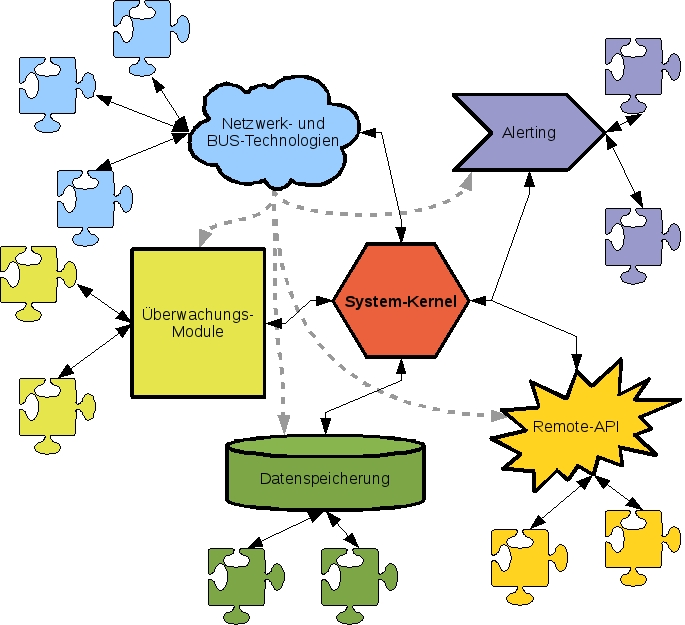
\includegraphics[width=0.8\linewidth]{images/theorie/Aufbau_Grundsystem}
  \caption[Aufbau der \"Uberwachungs-Software]{Das \"Uberwachungs-System bietet rund um den zentralen System-Kernel verschiedene Funktionen f\"ur unterschiedliche Bereiche an. Diese verschiedenen Bereiche stellen jeweils Container f\"ur Module dar, welche sowohl in bin\"arer Form als auch als LUA-Skript vorliegen k\"onnen. Eine Modul-Instanz kann beim System-Kernel eine Instanz eines anderen Moduls anfragen und dieses direkt nutzen. Dieser Prozess ist mit den "`Netzwerk- und BUS-Technologien"'-Modulen schematisch dargestellt.}
  \label{fig:praxis-aufbau}
\end{figure}

\subsection{System-Kernel} \label{sec:praxis-basis-kernel}
Die zentrale Schnittstelle\index{System-Kernel}, der System-Kernel, ist grunds\"atzlich verantwortlich f\"ur die komplette Thread-Verwaltung\index{Thread-Verwaltung} sowie f\"ur die Kommunikation zwischen den Threads und den Modulen.

Nach dem Start des Programms wird eine Instanz des System-Kernels angelegt und die verschiedenen Modul-Container\index{Modul-Container} geladen. Sind alle Modul-Container erfolgreich geladen, wird zuerst der \texttt{MainSystem}-Thread\index{MainSystem}, anschliessend der \texttt{Monitoring}-Thread\index{Monitoring} und zum Schluss der \texttt{MainListener}-Thread\index{MainListener} gestartet. Die verschiedenen Threads werden in den nachfolgenden Kapiteln beschrieben.

Durch einen Z\"ahler, welcher beim Erstellen einer Modul-Container Instanz inkrementiert wird, sowie einem Signal, welches der Conatiner sendet, wenn alles geladen ist, kann gepr\"uft werden, ob alle Container geladen worden sind. Vor der Initialisierung wird also ein Z\"ahler inkrementiert sowie eine Funktion des System-Kernels an das Signal gebunden (Codeblock \ref{alg:praxis-basis-kernel-container-init1}). Konnten alle Module erfolgreich geladen werden, wird vom Container das Signal aufgerufen und dadurch die vorg\"angig daran gebundene Funktion. Diese Funktion dekrementiert den Z\"ahler und f\"uhrt weitere Ladeaktionen aus wenn dieser wieder bei $0$ angelangt ist (Codeblock \ref{alg:praxis-basis-kernel-container-init2}).

Der Thread des \texttt{MainSystem} dient vor allem dazu, eine Asynchrone MessageQueue\index{MessageQueue} ab zu arbeiten. Nachrichten in dieser Queue k\"onnen von unterschiedlichen Stellen eingespiesen werden. Eine Nachricht\index{Nachricht} besteht immer aus einem Kommando und optionalen Daten (siehe Codeblock \ref{alg:praxis-basis-kernel-msg}). Die Nachrichten werden nach dem FIFO-Prinzip (first in first out) abgearbeitet, sie werden also der Reihe nach ausgelesen und das darin enthaltene Kommando ausgef\"uhrt. Sind keine Daten mehr in der \texttt{MessageQueue}, wird der Vorgang f\"ur 100ms pausiert. In einer zuk\"unftigen Version kann angedacht werden, anstelle der Pausierung f\"ur 100ms diesen komplett zu stoppen und beim einspeisen einer Nachricht ein Signal ab zu setzen, welches den Thread wieder aufweckt.

Eine weitere Aufgabe des \texttt{MainSystem}-Threads\index{MainSystem} sind diverse Aufr\"aumarbeiten. Bei einem Host-Discovery\index{Host-Discovery}\index{Discovery} wird beispielsweise eine Objekt-Liste mit verschiedenen Discovery-Prozessen (siehe Kapitel \ref{sec:praxis-basis-discovery}) angelegt. Ist ein Prozess abgeschlossen, muss dieser beendet und wieder freigegeben werden.

\subsubsection{Globale Kernel-Funktionen} \label{sec:praxis-basis-global}
Zur Kommunikation mit den unterschiedlichen Modulen und den verschiedenen Modul-Containern\index{Modul-Container} stehen im System-Kernel\index{System-Kernel} einige \"offentliche Funktionen zur Verf\"ugung:
\begin{description}
\item[exit](): Beendet alle Threads und das Programm\index{Funktionen!exit}

\item[getComm](string name): Erzeugt ein neues Kommunikations-Modul (ICommModule) und gibt dieses zur Verwendung zur\"uck.\index{Funktionen!getComm}\index{Modul!Kommunikation}

\item[getData](string name): Erzeugt ein neues Datenbank-Modul (IDataModule) und gibt dieses zur Verwendung zur\"uck.\index{Funktionen!getData}\index{Modul!Daten}

\item[getAlert](string name): Erzeugt ein neues Alert-Modul (IAlertModule) und gibt dieses zur Verwendung zur\"uck.\index{Funktionen!getAlert}\index{Modul!Alerting}

\item[getRemote](string name): Erzeugt ein neues Remote-API-Modul (IRemoteModule) und gibt dieses zur Verwendung zur\"uck.\index{Funktionen!getRemote}\index{Modul!Remote-API}

\item[getMonitor](string name): Erzeugt ein neues Monitoring-Modul (IMonitorModule) und gibt dieses zur Verwendung zur\"uck.\index{Funktionen!getMonitor}\index{Modul!Monitoring}\index{Monitoring!Modul}

\item[logMonitoring](string plugin, string host, string$\left[ \right]$ result): Nimmt eine Meldung von einem \"Uberwachungsmodul entgegen und speichert diese in allen konfigurierten Datenbanken ab.\index{Funktionen!logMonitoring}\index{Monitoring!Nachricht speichern}

\item[sendAlert](string plugin, string host, int timeout, string subject, string short\_message, string message, string$\left[ \right]$ attachment=null): Nimmt eine Fehlermeldung entgegen und sendet einen Alert wenn dies erforderlich ist. Basierend auf dem Plugin und dem Host kann gepr\"uft werden, ob ein Alert schon versendet worden ist oder nicht. Die Parameter werden 1:1 an das entsprechende Alert-Modul \"ubergeben. Je nach Art der Nachricht werden die einzelnen Daten dabei gek\"urzt oder erst gar nicht versendet.\index{Funktionen!sendAlert}\index{Monitoring!Alert speichern}

\item[getDiscoverServiceList](): Gibt eine Liste mit allen Diensten zur\"uck, auf welche ein System gepr\"uft werden soll, wenn dieses beim Auto-Discovery gefunden worden ist. Die Liste besteht aus \texttt{Helper.NetService}-Datens\"atzen.\index{Funktionen!getDiscoverServiceList} Die \texttt{Helper.NetService}-Datenstruktur ist im Anhang \ref{alg:praxis-basis-netservice} zu sehen.

\item[setDiscoveredHosts](Helper.NetService$\left[ \right]$ list): Systeme, welche durch ein AutoDiscovery gefunden und untersucht worden sind, k\"onnen \"uber diese Funktion dem System mitgeteilt werden. Die Systeme m\"ussen als \texttt{Helper.NetService} vorliegen.\index{Funktionen!setDiscoveredHosts}

\item[getDataFile](string file\_name): Gibt ein \texttt{File}-Objekt f\"ur eine Datei oder ein Verzeichnis innerhalb des "`data"'-Verzeichnisses zur\"uck.\index{Funktionen!getDataFile}

\item[getPath](string$\left[ \right]$ name): Gibt ein Unterverzeichnis als String zur\"uck. Die Unterverzeichnisse m\"ussen als String-Array \"ubergeben werden.\index{Funktionen!getPath}

\item[getFile](string$\left[ \right]$ path, string name): Gibt eine Datei als String zur\"uck. Die Unterverzeichnisse m\"ussen als String-Array \"ubergeben werden.\index{Funktionen!getFile}
\end{description}

\subsubsection{Modul-Container / PluginRegistrar} \label{sec:praxis-basis-kernel-container}
Ein Modul-Container\index{Modul-Container} ist prinzipiell eine einfache typisierte Liste, welche ein bin\"ares Modul laden und Instanzen von diesem zur\"uckgeben kann. Diese typisierte Liste wird implementiert durch den \texttt{PluginRegistrar}. Beim Instanzieren muss das Verzeichnis angegeben werden, welches die Module beinhaltet, die geladen werden sollen. Existiert das angegebene Verzeichnis, werden alle Unterverzeichnisse der Reihe nach durchlaufen und in diesen nach der Datei \texttt{libplugin.so}\index{libplugin.so} gesucht. Existiert eine solche Datei, wird sie in den Speicher geladen und versucht \"uber die Funktion \texttt{register\_plugin(Module module, PluginRegistrar registrar)}\index{Funktionen!register\_plugin} das Plugin zu initialisieren. Diese Einstiegsfunktion muss das Plugin durch den Typen, den Pfad sowie einen Identifier im entsprechenden \texttt{PluginRegistrar}\index{PluginRegistrar} speichern. Wird keine solche Einstiegsfunktion gefunden, kann das plugin nicht geladen werden.

Bei der Initialisierung eines \texttt{PluginRegistrar} muss immer auch ein Interface angegeben werden, welches f\"ur die geladenen Module verwendet wird. Zus\"atzlich muss auch noch ein Pointer auf das \texttt{MainSystem} \"ubergeben werden, so dass die Module und auch der Container Anfragen an den System-Kernel stellen k\"onnen (siehe Codeblock \ref{alg:praxis-basis-kernel-container-init1}).

Damit der \texttt{PluginRegistrar}\index{PluginRegistrar} andere Komponenten dar\"uber informieren kann, dass nun alle Module geladen sind, wird nach dem Laden ein Signal abgesetzt. Auf dieses Signal k\"onnen sich andere Komponenten Funktionen registrieren, welche anschliessend aufgerufen werden (siehe Codeblock \ref{alg:praxis-basis-kernel-container-init1} und \ref{alg:praxis-basis-kernel-container-init2}). Durch diese Funktionalit\"at stellt der System-Kernel fest, wann alle Module geladen sind und mit dem Laden von anderen Komponenten und Threads weitergemacht werden kann.

\begin{figure}[h]
 \lstset{language=[ISO]C++}
 \begin{lstlisting}[label=alg:praxis-basis-kernel-container-init1,caption={[Initialisierung eines Modul-Containers]Dieser Modul-Container l\"adt alle Module im Verzeichnis \texttt{pnetwork} und ruft nach dem erfolgreichen Laden die Funktion \texttt{modulesLoaded} (siehe Codeblock \ref{alg:praxis-basis-kernel-container-init2}) aus dem MainSystem auf. Durch den \texttt{load()}-Aufruf wird der Ladevorgang gestartet.}]
// Counter to check if all Container are loaded
registrars_loaded++;

comm = new PluginRegistrar<ICommModule>("pnetwork", this);
comm.complete.connect(modulesLoaded);
comm.load();
 \end{lstlisting}
\end{figure}

\begin{figure}[h]
 \lstset{language=[ISO]C++}
 \begin{lstlisting}[label=alg:praxis-basis-kernel-container-init2,caption={[Pr\"ufung, ob bereits alle Modul-Container geladen sind]Eine Funktion, die an das \texttt{complete}-Signal des \texttt{PluginRegistrar} gebunden wird, muss \"uber den Parameter \texttt{string path} verf\"ugen. Dieser beinhaltet den Pfad der Module. Diese Implementierung zeigt, wie gew\"ahrleistet wird, dass erst nach dem Laden aller Container gewisse Funktionen ausgef\"uhrt werden.}]
private void modulesLoaded(string path) {
  registrars_loaded--;

  // All modules are loaded
  if (registrars_loaded <= 0) {
    ...
  }
}
 \end{lstlisting}
\end{figure}

Jedes Plugin, das geladen wird, registriert sich entweder \"uber die Funktion \texttt{addPlugin(""IMainModule ""plugin)} oder \"uber \texttt{addInstance(""Type t, ""string path, ""string identi""fier)} bei dem Modul-Container. Ein Plugin kann sich dadurch als "`bereits instanziert"' oder als "`noch zu instanzieren"' registrieren. Durch die Festlegung, dass ein \"Uberwachungssystem so wenig Resourcen wie m\"oglich belegen darf, sollten bereits instanzierte Plugins so wenig wie m\"oglich genutzt werden, da diese beim Systemstart komplett in den Speicher geladen werden und dort verbleiben (w\"ahrend dem die anderen geladen und anschliessend wieder freigegeben werden). Zudem sollte ein solches Plugin als Singelton implementiert werden, denn es kann nur einmal im System bestehen.

Plugins, welche \"uber die \texttt{addInstance(...)}-Funktion registriert werden, k\"onnen zu einem beliebigen Zeitpunkt instanziert werden. Daf\"ur notwendig ist lediglich der Typ, welcher der Funktion \"ubergeben wird. Damit dies jedoch funktioniert, muss beim Laden der Datei \texttt{libplugin.so} angegeben werden, dass dieses Modul speicherresistent sein muss, ansonsten wird der Speicher mit den Modul-Informationen beim verlassen der Funktion wieder freigegeben. Codeblock \ref{alg:praxis-basis-kernel-container-load} zeigt einen schematischen Ablauf des Ladeprozesses. Bei Zeile 4 und 7 wird das Plugin \"uber ein Modul geladen und auf Zeile 9 definiert, dass die Informationen speicherresistent gehalten werden m\"ussen. Anschliessend wird bei Zeile 12 gepr\"uft, ob die Einstiegsfunktion \texttt{register\_plugin} existiert. Ist dies nicht der Fall, wird abgebrochen. Auf den Zeilen 16 und 17 wird der Typ der Einstiegsfunktion definiert und diese anschliessend bei Zeile 18 aufgerufen.

\begin{figure}[h]
 \lstset{language=[ISO]C++}
 \begin{lstlisting}[label=alg:praxis-basis-kernel-container-load,caption={[Beispiel zum Laden eines bin\"aren Moduls]Ablauf zum Laden eines bin\"aren Modules. Zuerst wird das Modul geladen, speicherresident gehalten, auf die Einstiegsfunktion gepr\"uft und diese, wenn gefunden, aufgerufen.}]
protected delegate Type RegisterPluginFunction(Module module,
                                    PluginRegistrar registrar);

string plugin_file = Module.build_path(
    Path.build_filename(module_dir.get_path(), plugin_name),
    "plugin");
Module module = Module.open(plugin_file,
                            ModuleFlags.BIND_LAZY);
module.make_resident();

void* function;
if (!module.symbol("register_plugin", out function)) {
  return;
}

RegisterPluginFunction register_plugin =
   (RegisterPluginFunction)function;
register_plugin(module, this);
 \end{lstlisting}
\end{figure}

Basierend auf dem Identifier\index{Plugin-Identifier}, welcher jedes Plugin pro Modul-Container\index{Modul-Container} eindeutig macht, kann der System-Kernel anschliessend eine Instanz eines Moduls anfragen. Ist das Plugin im angefragten ModulContainer vorhanden, wird basierend auf dem Typen ein neues Objekt erstellt, auf das dem \texttt{PluginRegistrar}\index{PluginRegistrar} zugrunde liegende Interface gecastet und zur\"uckgegeben (siehe Codeblock \ref{alg:praxis-basis-kernel-container-get}). Wird ein nicht existierendes Modul angefragt, wird anstelle dessen \texttt{NULL} zur\"uckgegeben. Es muss also immer zuerst gepr\"uft werden, ob die angefragte Instanz \texttt{NULL} ist oder nicht. Ansonsten kann es zu Problemen bei der Programm-Ausf\"uhrung und zu Instabilit\"aten kommen (\texttt{NULL}-Pointer Exceptions, Assertions, etc.).

\begin{figure}[h]
 \lstset{language=[ISO]C++}
 \begin{lstlisting}[label=alg:praxis-basis-kernel-container-get,caption={[Erstellen einer neuen Instanz eines Moduls]Nachdem alle Module geladen worden sind, kann ein Modul \"uber die Funktion \texttt{getPlugin(string name)} angefordert werden. Existiert ein Plugin mit dem Identifier \texttt{name}, wird eine Instanz von diesem zur\"uckgegeben. Vor der R\"uckgabe wird das neu erstellte Objekt auf das dem PluginRegistrar zugrundegelegte Interface gecastet.}]
public class PluginRegistrar<T> : Object {
  public T? getPlugin(string name) {
    if (pluginExists(name))
      return (T)new Object(ModuleType(name));
    return null;
  }
}

// Get an ICMP-Plugin
ICommModule mod = comm.getPlugin("icmp");
 \end{lstlisting}
\end{figure}

\subsubsection{Monitoring-Thread} \label{sec:praxis-basis-kernel-monitor}
Damit weder ein anderes System noch anderen Komponenten der Software vom Monitoring ausgebremst oder unterbrochen werden, wird dieses in einen eigenen Thread ausgelagert. Das Monitoring\index{Monitoring} l\"auft somit parallel zu allen anderen Funktionen, kann jedoch den System-Kernel ungehindert verwenden.

Nach dem Start des Threads durch den System-Kernel\index{System-Kernel} werden alle Monitoring-Systeme und Module geladen, konfiguriert und im Speicher in einer Liste gehalten. In regelm\"assigen Abst\"anden wird dann diese Liste durchlaufen und geschaut, welche Pr\"ufung aktuell ansteht. Ob ein System zum aktuellen Zeitpunkt durch das momentane Modul gepr\"uft werden soll oder muss, wird dabei nicht vom Monitoring-Thread bestimmt, sondern vom Modul selbst. Jedes Modul weiss, wann es zuletzt ausgef\"uhrt worden ist und wann der n\"achste Zeitpunkt f\"ur eine Pr\"ufung ist (siehe Kapitel \ref{sec:praxis-basis-monitor}). Der Monitoring-Thread schaut grunds\"atzlich nur, ob das Modul aktuell eine Pr\"ufung durchf\"uhrt oder nicht sowie ob der Zeitpunkt (Timestamp) des Moduls abgelaufen ist. Basierend auf diesen zwei Tatsachen kann dann gesagt werden, ob eine Pr\"ufung ansteht oder nicht.

Der Monitoring-Thread kann durch den System-Kernel \"uber das Property \texttt{pause} unterbrochen respektive pausiert werden. Dies hat den Sinn, dass wenn zum Beispiel neu zu \"uberwachende Hosts eingef\"ugt werden, diese vom Monitoring-Thread zuerst geladen werden m\"ussen (definiert \"uber das Property \texttt{reload}). Damit es bei solchen Aktionen nicht zu Datenfehlern kommt, wird bei einem Rebuild der \"Uberwachung dieser Thread pausiert und anschliessend wieder neu gestartet, respektive der Mainloop des Threads wird wieder ausgef\"uhrt.

\subsubsection{Kommunikations-Thread} \label{sec:praxis-basis-kernel-listener}
Damit die verschiedenen \"Uberwachungssysteme untereinander kommunizieren k\"onnen, wird der MainListener-Thread\index{MainListener} gestartet, welcher f\"ur diese Kommunikation zust\"andig ist. Nachrichten unter den Systemen werden mit dem verbindungslosen Protokoll UDP versendet, damit ein allenfalls nicht laufendes System nicht die komplette \"Uberwachung ausbremst\footnote{Bei TCP-Verbindungen kann es vorkommen, dass eine Verbindung, welche nicht korrekt oder komplett aufgebaut werden kann, diese erst nach einem definierten Timeout geschlossen wird oder so lange versucht wird diese korrekt auf zu bauen bis eben dieses Timeout abgelaufen ist. W\"ahrend dieser Zeit ist das System ausgebremst, da es ja eine Antwort erwartet.}. Zudem darf ein System nicht ausgebremst werden, wenn ein anderes System ausgelastet ist und das erstellen einer Antwort mehrere Sekunden in Anspruch nimmt. Bei einer TCP Verbindung wird immer eine Antwort ben\"otigt, was bedeutet, dass das anfragende System ausgebremst wird f\"ur die Dauer welche das ausgelastete System f\"ur die Erstellung der Antwort braucht. Bei UDP k\"onnen Antworten nicht direkt sondern m\"ussen ebenfalls als UDP-Paket versendet werden. Somit spielt es bei UDP keine Rolle, wie lange ein System f\"ur die Erstellung einer Antwort braucht.

Der Thread beinhaltet einen UDP-Listener-Socket\index{UDP}, welcher auf alle vorhandenen NICs (Network Interface Card) gebunden ist. Das Problem bei UDP-Sockets ist, dass immer angegeben werden muss, wie viele Bytes empfangen werden sollen. Aus diesem Grund k\"onnen Daten nicht einfach so wie sie vorliegen gesendet werden, sondern m\"ussen gegebenenfalls in mehrere Pakete aufgeteilt und empfangen werden. Eine Gr\"osse, welche sich bei UDP etabliert hat, sind 1024 Bytes\index{UDP-Paketgr\"osse}. Diese Anzahl scheint Tests zufolge auf den meisten Systemen performant zu laufen, w\"ahrend gr\"ossere Pakete bei gewissen Betriebssystemen Schwierigkeiten bereiten\footnote{Ein UDP-Paket von 2048 Bytes brauchte auf einem WindowsXP fast doppelt so lange wie zwei UDP-Pakete mit 1024 Byte.}.

Aus diesem Grund musste ein einfaches und simples Datenformat definiert werden, welches Abbildung \ref{fig:praxis-basis-kernel-listener-format} aufzeigt. Aktuell werden alle Daten als Klartext versendet, was nicht nur viel Datenmenge bedeutet, sondern auch sicherheitskritisch sein kann. Kommende Versionen der Software sollten nicht nur eine komprimierte oder bin\"are Version des Protokolls aufweisen, sondern auch eine Authentifizierung und/oder sogar eine Verschl\"usselung.

\begin{figure}[h]
  \centering
  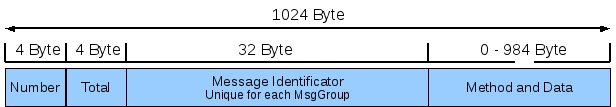
\includegraphics[width=0.8\linewidth]{images/theorie/Aufbau_Kommunikation_Format}
  \caption[Datenformat einer AMoDS-Meldung]{Jeweils 4 Zeichen definieren die aktuelle Nachrichtennummer und die totale Anzahl an Nachrichten. Die folgenden 32 Zeichen werden als Nachrichten-UID interpretiert. Die restlichen 984 Zeichen sind die Daten, welche das Kommando getrennt durch einen Doppelpunkt von den Daten beinhalten.}
  \label{fig:praxis-basis-kernel-listener-format}
\end{figure}

Alle UDP-Pakete, die auf einem definierten Port eingehen, werden empfangen und auf G\"ultigkeit \"uberpr\"uft. Ist ein Paket g\"ultig, wird es in die einzelnen Bereiche unterteilt und in einer Datenstruktur gespeichert. Diese Datenstruktur wird so lange im Speicher gehalten, bis alle Nachrichten eingetroffen sind. In einer finalen Version, werden alle empfangenen Pakete beim Absender best\"atigt und in regelm\"assigen Abst\"anden die vorhandenen, noch nicht kompletten Pakete, bei diesem reklamiert.

TCP-Verbindungen k\"onnen einfach \"uber die Konsole zum Beispiel mit dem \texttt{telnet}-Kommando ausgef\"uhrt und getestet werden. Dies ist bei UDP leider nicht der Fall. Eine gute Alternative bietet hierzu NetCat\cite{netcat}\index{NetCat}. Mittels diesem k\"onnen UDP-Pakete auf einfache Art und Weise gesendet und empfangenen werden. Es k\"onnen so andere Systeme und dessen Kommunikation simuliert werden und einfache Nachrichten\index{Nachricht} wie Kommandos an ein System gesendet werden.

Durch den Befehl "`\texttt{echo '1   1   74957e5872f8b604d2774b79e8c7e8c2""monitor: 192.""168.""22.""70 192.""168.""22.""77' \textbar nc -q 1 -u 192.168.22.27 1611}"' kann zum Beispiel unter Linux/Unix dem \"Uberwachungs-System \texttt{192.168.22.27} mitgeteilt werden, dass es f\"ur die Systeme \texttt{192.168.22.70} und \texttt{192.168.22.77} zust\"andig ist. Entsprechend verh\"alt es sich mit den anderen Kommandos.

Eine Liste mit allen Kommandos und deren Daten, ist in Tabelle \ref{tbl:praxis-basis-kernel-remote} im Anhang gelistet.

\subsection{Kommunikations-Plugins} \label{sec:praxis-basis-comm}
\index{Modul!Kommunikation}Kommunikations-Module haben die Aufgabe, Verbindungen mit anderen Systemen her zu stellen sowie deren Antworten zu empfangen und weiter zu reichen. Dabei kann es sich sowohl um ein Netzwerk-Protokoll als auch um ein Bus-System oder eine lokale Datenanfrage handeln. Alle Kommunikations-Module werden vom Interface \texttt{ICommModule} abgeleitet (siehe Codeblock \ref{alg:praxis-basis-icommodule}), welches wiederum eine Implementation des Interfaces \texttt{IMainModule} voraussetzt (siehe Codeblock \ref{alg:praxis-basis-imainmodule}).

Das Interface der Kommunikations-Module ist so gehalten, dass nicht bekannt sein muss, \"uber was f\"ur eine Technologie die Daten versendet und empfangenen werden. Jegliche Einstellungen werden \"uber die Methode \texttt{setParam(string key, string value)} definiert. Dabei kann jedes Modul selber entscheiden, welche Parameter es anschliessend verwendet und welche nicht.

Neben Funktionen zur einfachen Datenanfrage und Daten\"ubermittlung sind auch drei Signale zur Eventbehandlung auf dem Interface enthalten. Dies ist zum einen das Signal \texttt{onError} f\"ur das Error-Handling sowie die zwei Daten-Signale \texttt{onData} und \texttt{onComplete}. Der Event \texttt{onData} wird aufgerufen, sobald Daten empfangen werden; \texttt{onComplete} erst wenn die Kommunikation beendet ist. Auf die Signale k\"onnen verschiedene Methoden gebunden werden, welche beim Auftreten des Events aufgerufen werden.

Nachdem ein Modul instanziert und alle notwendigen Parameter gesetzt worden sind, kann durch die Funktion \texttt{send(string? data="`"')} eine Anfrage gestartet werden. Optional k\"onnen beim Senden noch Daten mit angegeben werden, welche jedoch nicht von allen Modulen genutzt werden m\"ussen.

Bei mehrstufigen Protokollen, wie zum Beispiel einer SMTP-Pr\"ufung, kann \"uber das \texttt{onData}-Signal eine Antwort empfangen, ausgewertet und durch einen erneuten Send-Aufruf auf die empfangenen Daten eingegangen werden. Besteht eine Anfrage nur aus einem Request, zum Beispiel ein ECHO-Ping, kann auch nur auf das \texttt{onComplete}-Signal eingegangen werden. Dieses beinhaltet alle empfangenen Daten als String-Array.

Das \texttt{onError}-Signal sollte grunds\"atzlich immer beachtet werden. Tritt ein Fehler auf, kann durch dieses Signal festgestellt werden, um was f\"ur einen Fehler es sich handelt und so zum Beispiel ein Alert versendet oder eine andere Methode ausprobiert werden.

\subsubsection{Liste von verf\"ugbaren Modulen} \label{sec:praxis-basis-comm-list}
Die Kommunikations-Module befinden sich im Unterverzeichnis \texttt{pnetwork}:
\begin{itemize}
 \item[\textbf{udp}] Sendet Daten \"uber einen UDP-Socket an einen Host. Ben\"otigt werden mindestens die Parameter "`host"' und "`port"' sowie die Daten beim Aufruf der Send-Funktion. Aktuell wird f\"ur eine eventuelle Antwort kein Socket ge\"offnet. In einer kommenden Version wird dies m\"oglich sein, um so zum Beispiel SNMP-Pr\"ufungen direkt durchf\"uhren zu k\"onnen.

 \item[\textbf{tcp}] Sendet Daten \"uber einen TCP-Socket und wartet eine Antwort ab. Ben\"otigt werden mindestens die Parameter "`host"' und "`port"' sowie die Daten beim Aufruf der Send-Funktion. Bei der aktuellen Version bestehen noch gewisse Schwierigkeiten bei der Pr\"ufung ob der Socket noch ge\"offnet ist oder nicht. Soll der Socket explizit geschlossen werden, kann dies durch einen "`send()"'-Aufruf (ohne Daten) forciert werden. Es kann also sein, dass momentan bei einer "`falschen"' Verwendung des TCP-Modules das \texttt{onComplete}-Signal nicht aufgerufen wird.

 \item[\textbf{snmp}] Pr\"uft das Vorhandensein eines Systems anhand einer \texttt{sysDescr}-OID-Anfrage. Ben\"otigt wird mindestens der Parameter "`host"'. Die aktuelle Version dieses Plugins funktioniert lediglich unter einem Unix-\"ahnlichen Betriebssystem und dem\\ \texttt{/usr/bin/snmpget}-Befehl.

 \item[\textbf{echo}] Sendet einen ECHO-Ping an ein System. Ben\"otigt wird mindestens der Parameter "`host"'. Die aktuelle Version verwendet den \texttt{ping}-Befehl aus dem Unterverzeichnis "`bin"'. Der Code des \texttt{ping}-Binaries wurde ebenfalls im Zuge der Bachelor-Thesis ausgearbeitet um eine Parser-freundlichere Ausgabe zu erhalten.

 \item[\textbf{arp}] Sendet ein ARP-Package auf das Netzwerk und wartet die Antwort ab. Ben\"otigt wird mindestens der Parameter "`host"'. Die aktuelle Version verwendet eine im Zuge der Bachelor-Thesis angepasste Version des Programms \texttt{arping2}, bei welchem alle Bindungen zu "`LibNet"' entfernt wurden\footnote{Die ben\"otigten Funktionen und Datenstrukturen von Libnet-1.1.5 wurden direkt in den C-Code von Arping-2.06 eingef\"ugt.} um so von weniger externen Bibliotheken abh\"angig zu sein.

 \item[\textbf{amods}] Sendet einen Befehl inklusive Daten an ein anderes \"Uberwachungs-System. Ben\"otigt wird mindestens der Parameter "`host"' und die Daten beim Aufruf der Send-Funktion. Auf ein eventuelles Antwort-Paket wird nicht eingegangen, denn dieses wird bereits vom \texttt{MainListener}-Thread abgefangen und verarbeitet.
\end{itemize}


\subsection{\"Uberwachungs-Plugins} \label{sec:praxis-basis-monitor}
\index{Modul!Monitoring}\index{Monitoring!Modul}Die \"Uberwachungsmodule sind f\"ur die \"Uberwachung eines lokalen oder entfernten Dienstes zust\"andig. Diese Module sind die einzigen, welche beim Start des Systems geladen und in einer Liste gehalten werden. Dabei wird pro System und Dienst ein Modul gebraucht. Die Konfiguration der einzelnen Module wird dabei vom System ausgelesen und bei der Instanzierung des Moduls gesetzt.

Alle \"Uberwachungsmodule m\"ussen das Interface \texttt{IMonitorModule} implementieren (siehe Codeblock \ref{alg:praxis-basis-imonitormodule}), welches wiederum das Interface \texttt{IMainModule} voraussetzt (siehe Codeblock \ref{alg:praxis-basis-imainmodule}). Mittels den Properties \texttt{running} und \texttt{next\_run} muss vor einer Pr\"ufung geschaut werden, ob diese gestartet werden soll. Durch die Methode \texttt{monitor()} wird die Pr\"ufung anschliessend ausgef\"uhrt. Der Aufruf der Monitor-Funktion sollte asynchron (\texttt{monitor.begin()}) gestartet werden, da ansonsten die restlichen Thread-Funktionen warten bis das Modul mit der Pr\"ufung fertig ist.

%In einer Kommenden Version kann auch angedacht werden, dass alle Pr\"ufungen vom gleichen Typen (ICMP\index{ICMP}, SNMP\index{SMTP}, etc.) oder Pr\"ufungen von einem Host in einem eigenen Thread laufen sollen. Inwieweit dies jedoch Sinnvoll ist, muss erst noch gepr\"uft werden.

Welche Kommunikations-Module von den \"Uberwachungsmodulen genutzt werden, liegt im Ermessen des Moduls. Diese werden bei Bedarf im System-Kernel\index{System-Kernel} angefragt, anschliessend konfiguriert, die Signale an Modul-Funktionen gebunden und dann Daten gesendet. Tritt bei der Verbindung ein Fehler auf, muss das \"Uberwachungsmodul entscheiden, ob eine erneute Pr\"ufung notwendig ist oder ob dem System-Kernel mitgeteilt werden soll, dass ein Fehler aufgetreten ist. Ob jedoch bei einem Fehler ein Alert gesendet wird oder nicht entscheidet nicht mehr das Modul, dies unterliegt der Hoheit des System-Kernels.

Wird eine \"Uberwachung erfolgreich durchgef\"uhrt und ohne Fehler abgeschlossen, wird dies dem System-Kernel durch ein Signal und einen Funktionsaufruf mitgeteilt. Dieser speichert die \"ubermittelten Daten sowie den Zeitpunkt der Pr\"ufung in der Datenbank.\index{Monitoring!Nachricht speichern}\index{Monitoring!Alert speichern}

Ist eine Pr\"ufung abgeschlossen - ob erfolgreich oder nicht - wird das Property \texttt{running} zur\"uckgesetzt und ein neuer Timestamp im Property \texttt{next\_run} gesetzt.

\subsubsection{Liste von verf\"ugbaren Modulen} \label{sec:praxis-basis-monitor-list}
Die Monitoring-Module befinden sich im Unterverzeichnis \texttt{pmonitor}:
\begin{itemize}
 \item[\textbf{icmp}] Pr\"uft das Vorhandensein eines Systems anhand eines ECHO-Pings. Erwartet als Konfiguration einen "`host"' und optional ein "`num"' f\"ur die Anzahl an Echo-Requests und ein optionales "`timeout"', welches die Anzahl Sekunden zwischen den einzelnen Pr\"ufungen definiert. Es wird das \texttt{echo}-Kommunikations-Plugin verwendet.

 \item[\textbf{smtp}] Pr\"uft einen EMail-Servers durch den Aufbau einer SMTP-Verbindung. Zur Pr\"ufung ist ein "`host"' und optional ein "`port"' Parameter notwendig sowie optional ein "`timeout"' und ein "`num"' f\"ur die Anzahl an Verbindungsversuchen. Zus\"atzlich muss mit dem Parameter "`mail\_from"' die Absender-EMail-Adresse und mit "`rcpt\_to"' die Empf\"anger-EMail-Adresse definiert werden. Wird \"uber "`user"' und "`password"' zus\"atzlich ein Benutzer und Passwort sowie eine Authentifizierungs-Methode mit "`auth\_method"' definiert, werden diese Daten ebenfalls genutzt zum Verbindungsaufbau. Die Pr\"ufung versendet kein EMail, es wird lediglich gepr\"uft, ob das Versenden m\"oglich ist\footnote{Ein EMail-Server wird gepr\"uft, indem eine Verbindung aufgebaut wird, ein Absender und Empf\"anger \"ubermittelt wird sowie optional noch eine Authentifizierung. Anschliessend wird die Verbindung abgebrochen mit dem Befehl \texttt{quit}.}. Es wird das \texttt{tcp}-Kommunikations-Plugin verwendet.

 \item[\textbf{http}] Pr\"uft ob der angegebene Webserver erreichbar ist oder nicht. Zur Pr\"ufung ist prinzipiell nur der "`host"' Parameter notwendig, optional kann noch ein "`port"' definiert werden. Das Modul pr\"uft den Server standardm\"assig mittels der Anfrage "`OPTIONS * HTTP/1.1"' auf dessen Erreichbarkeit. Durch die Angabe des Parameters "`method"', welcher die HTTP-Methode definiert (GET, POST, OPTIONS, HEAD) und einer "`url"', kann aber auch die Funktionst\"uchtigkeit eines Webdienstes abgefragt werden. Bei der POST-Methode k\"onnen zus\"atzlich noch Daten \"uber den Parameter "`content"' \"ubergeben werden, welche bei allen anderen Methoden nicht beachtet werden. Als Auswertungskriterium dient in jedem Fall nur die erste Zeile der Antwort, welche \"ublicheweise den Status als Zahl und Text beinhaltet: "`HTTP/1.0 \textbf{200 OK}"' oder bei einem Fehler "`HTTP/1.0 \textbf{400 Bad Request}"'.  Es wird das \texttt{tcp}-Kommunikations-Plugin verwendet.
\end{itemize}

\subsection{Datenspeicherungs-Plugins} \label{sec:praxis-basis-data}
\index{Modul!Daten}Die Module zur Datenspeicherung werden genutzt, um Daten in einer Datenbank oder auf einem entfernten Server ab zu legen und wieder aufzurufen. Das Datenmodell der einzelnen Tabellen wurde dabei absichtlich sehr einfach gehalten (Erste Normalform). Es k\"onnen dadurch nicht nur Datenbanken verwendet werden, welche SQL verstehen, sondern auch andere Datenspeicherungen wie zum Beispiel einfache XML-Dateien. Die vorhandenen Tabellen und Schemata sind im Anhang aufgef\"uhrt, siehe Tabelle \ref{tbl:praxis-basis-data-table_conf}, \ref{tbl:praxis-basis-data-table_netw}, \ref{tbl:praxis-basis-data-table_hosts}, \ref{tbl:praxis-basis-data-table_modules}, \ref{tbl:praxis-basis-data-table_monitor}, \ref{tbl:praxis-basis-data-table_alert} und \ref{tbl:praxis-basis-data-table_alertsent}.

Alle Datenmodule m\"ussen das Interface \texttt{IDataModule} implementieren (siehe Codeblock \ref{alg:praxis-basis-idatamodule}), welches wiederum das Interface \texttt{IMainModule} voraussetzt (siehe Codeblock \ref{alg:praxis-basis-imainmodule}).

Im \texttt{IDataModule}-Interface sind noch weitere spezielle Konstanten und Datentypen definiert. Die Konstanten \texttt{TABLE\_XX} und \texttt{SCHEMA\_XX} werden ben\"otigt um die Tabellen und deren Felder zu definieren. Die verschiedenen Tabellen werden durch die Enumeration \texttt{DataType} definiert (\texttt{CONF, MONITOR, ALERT, ...}). Jede so definierte Tabelle muss vom Datenmodul bei der Initialisierung gepr\"uft und gegebenenfalls erstellt werden. In einem ersten Schritt muss vom Plugin, basierend auf der Schema-Definition und des Datentypen \texttt{SchemaField}\footnote{Der Datentyp \texttt{SchemaField} beinhaltet alle notwendigen Daten um mittels SQL eine Tabelle erstellen zu k\"onnen.}, eine Liste mit allen Feldern erstellt werden, welche auf der Tabelle vorhanden sein m\"ussen. Um diesen Prozess zu vereinfachen, ist auf der \texttt{SchemaField}-Struktur eine Methode vorhanden, welche einen Schema-Definitions-String parst und wiederum ein \texttt{SchemaField} zur\"uck gibt. Die Erstellung dieser Schema-Definition wurde durch das evolution\"are Entwicklungsmodell so geboren, wird jedoch in einer kommenden Version direkt definiert werden, um das Laden resourcen-schonender zu gestalten.

Um ein Datenmodul zu verwenden, muss nach der Initialisierung definiert werden, um was f\"ur Daten sich das Plugin k\"ummern soll und in welcher Tabelle diese vorhanden sind. Die Definition des Typs geschieht \"uber das Property \texttt{data\_type}, welches als Wert einen \texttt{DataType} erwartet. Anschliessend kann \"uber die \texttt{open(string db\_name)}-Methode die Datenbank verbunden werden.

Um Daten zu lesen, stellt das Interface die Methoden \texttt{setWhere(""string field, ""string value)}\footnote{Die Methode \texttt{setWhere} wird genutzt um eine oder mehrere Bedingungen f\"ur eine Datenselektion zu definieren. Die Angaben haben keinen Einfluss auf das L\"oschen, Einf\"ugen und Aktualisieren von Datens\"atzen.} sowie \texttt{select(""string? fields="`"', ""string? groupedBy="`"')} zur Verf\"ugung. \"Uber diese Methoden k\"onnen Bedingungen sowie die Felder und Gruppierungen angegeben werden, welche aktuell ben\"otigt werden. Anschliessend kann \"uber die Methode \texttt{hasNext()}, \texttt{getCurrent()} sowie \texttt{getValue(""string field)} auf die Felder und deren Werte zugegriffen werden (Siehe Codeblock \ref{alg:praxis-basis-idatamodule-use} f\"ur ein Beispiel).

\begin{figure}[h]
 \lstset{language=[ISO]C++}
 \begin{lstlisting}[label=alg:praxis-basis-idatamodule-use,caption={[Beispiel zur Verwendung eines Datenmoduls]Beispiel: Verwendung eines Datenmoduls zum Auslesen aller Parameter zur Konfiguration eines \"Uberwachungsmodules. Nach dem das Modul geladen ist, wird definiert, dass Daten aus der \texttt{MODULES} Tabelle geladen werden sollen, und zwar nur jene, welche im Feld \texttt{host} und \texttt{module} entsprechende Werte beinhalten. \"Uber die Schlaufe und die Funktion \texttt{hasNext()} werden alle Datens\"atze ausgelesen und die Werte "`key"' und "`value"' zur Parametrierung eines anderen Modules genutzt.}]
string dbf = getDataFile("config.sqlite").get_parse_name();
IDataModule conf = data.get_plugin("sqlite");
if (conf != null) {
  conf.data_type = IDataModule.DataType.MODULES;
  conf.setWhere("host", host);
  conf.setWhere("module", module);
  if (conf.open(dbf) && conf.select()) {
    while (conf.hasNext()) {
      // "m" is an IMonitorModule Instance
      m.setParam(mod_conf.getValue("key"),
                 mod_conf.getValue("value"));
      // ...
    }
  }
}
 \end{lstlisting}
\end{figure}

Um Daten \"uber ein Datenmodul zu speichern, wird nur die Methode \texttt{save(""IData""Module.""DataSet[] values, ""IData""Module.""DataSet[]? ""where=null)} ben\"otigt. Die Felderliste \texttt{values} beinhaltet dabei alle Felder und die dazugeh\"orenden Werte f\"ur einen Datensatz. Wird keine Liste mit Bedingungen angegeben (\texttt{where}-Parameter), wird ein neuer Datensatz eingef\"ugt. Andererseits werden alle Datens\"atze aktualisiert, welche mit der Bedingungsliste \"ubereinstimmen. \"Uberschriebene Daten k\"onnen nicht wiederhergestellt werden. Ein Beispiel wie ein Datensatz eingef\"ugt/aktualisiert werden kann ist in Codeblock \ref{alg:praxis-basis-idatamodule-ins} zu sehen.

\begin{figure}[h]
 \lstset{language=[ISO]C++}
 \begin{lstlisting}[label=alg:praxis-basis-idatamodule-ins,caption={[Beispiel zum Speichern von Daten \"uber ein Datenmodul]Beispiel: Zuerst wird ein neuer Datensatz in die Modules-Tabelle eingef\"ugt. Anschliessend werden alle Datens\"atze aktualisiert, welche im Feld "`host"' und "`key"' entsprechende Werte haben.}]
string dbf = getDataFile("config.sqlite").get_parse_name();
IDataModule conf = data.get_plugin("sqlite");
if (conf != null) {
  // Data-Structure with all fields and values to use for a save/update
  IDataModule.DataSet[] dataSet = new IDataModule.DataSet[] {
    IDataModule.DataSet() { field="module", value="icmp" },
    IDataModule.DataSet() { field="host", value=host },
    IDataModule.DataSet() { field="key", value="timeout" },
    IDataModule.DataSet() { field="value", value="10" }
  };

  conf.data_type = IDataModule.DataType.MODULES;

  // Insert a new DataSet
  conf.save(dataSet);

  // Update an existing DataSet based on the second Data-Structure
  conf.save(dataSet, new IDataModule.DataSet[] {
    IDataModule.DataSet() { field="host", value=host },
    IDataModule.DataSet() { field="key", value="timeout" }
  });
}
 \end{lstlisting}
\end{figure}

Sollen Daten gel\"oscht werden, kann dies \"uber die Funktion \texttt{delete(""IData""Module.""DataSet[] ""where)} gemacht werden. Es werden alle Datens\"atze entfernt, welche den angegebenen Bedingungen entsprechen. Wenn alle Datens\"atze einer Tabelle entfernt werden sollen, kann dies durch die Funktion \texttt{empty()} gemacht werden. Gel\"oschte Daten k\"onnen nicht wiederhergestellt werden.

\subsubsection{Liste von verf\"ugbaren Modulen} \label{sec:praxis-basis-data-list}
Die Datenbank-Module befinden sich im Unterverzeichnis \texttt{pdata}:
\begin{itemize}
 \item[\textbf{sqlite}] Die Datenspeicherung erfolgt \"uber eine Sqlite3-Datenbank im Verzeichnis "`data"'.
\end{itemize}

\subsection{Alerting-Plugins} \label{sec:praxis-basis-alert}
\index{Modul!Alerting}Alerting-Module werden verwendet um Meldungen \"uber verschiedene Kan\"ale zu versenden. Dabei kann von den verschiedenen Kan\"alen nicht immer gew\"ahrleistet werden, dass eine Meldung auch wirklich versendet worden ist, oder dass dies gepr\"uft werden kann. Daher wird grunds\"atzlich ein erfolgreiches Versenden als Gegeben angenommen.

Ein Alert-Modul wird definiert durch das Interface \texttt{IAlertModule} (siehe Codeblock \ref{alg:praxis-basis-ialertmodule}), welches ebenfalls die Implementierung des \texttt{IMainModule} voraussetzt (siehe Codeblock \ref{alg:praxis-basis-imainmodule}). Ein Alert-Modul ist eines der einfachsten, da es lediglich dazu da ist, eine Nachricht zu versenden und anschliessend ein Signal aufzurufen. Die Pr\"ufung, ob und wann ein Alert schon versendet worden ist, muss vom System-Kernel entschieden werden.

Das Senden eines Alerts unterliegt dabei folgendem Schema: Der System-Kernel\index{System-Kernel} nimmt eine Anfrage zum Versenden einer Nachricht entgegen. Anhand der Daten, dem Typ und dem Schweregrad entscheidet dieser basierend auf der Konfiguration, \"uber welches Modul und an welche(n) Empf\"anger eine Nachricht versendet werden soll. Ein Alert-Modul wird erstellt und das Signal \texttt{onSent} des Moduls an eine Funktion gebunden sowie die Konfiguration mittels der Methode \texttt{setParam(string key, string value)} definiert. Anschliessend werden die Daten dem Modul zum Senden \"ubergeben. Nach dem die Daten vom Modul versendet worden sind, wird der \texttt{onSent}-Event mit dem Empf\"anger, einem Status und dem Alert-UID aufgerufen. Optional kann noch eine Meldung \"ubergeben werden.

Kann bei der verwendeten Technik nicht festgestellt werden, ob die Daten erfolgreich versendet worden sind, wird der \texttt{onSent}-Event einfach direkt nach dem Versenden aufgerufen.

Tritt beim Versenden der Nachricht ein Fehler auf, wird der \texttt{onSent}-Event ebenfalls aufgerufen. In diesem Fall jedoch mit einem Fehler-Code und einer Fehlernachricht.

Die Methode, welche an das \texttt{onSent}-Signal gebunden wird, muss anschliessend entscheiden, ob ein weiterer Alert versendet werden muss oder nicht. Dies hat ebenfalls nicht das Alert-Modul zu entscheiden.

\subsubsection{Liste von verf\"ugbaren Modulen} \label{sec:praxis-basis-alert-list}
Die Alerting-Module befinden sich im Unterverzeichnis \texttt{palert}:
\begin{itemize}
 \item[\textbf{email}] Ein Alert wird mittels EMail versendet. Die Plugin-Konfiguration erfordert mindestens einen Host sowie eine oder mehrere Empf\"anger-Adressen. Optional kann ein Port sowie eine Absender-Adresse, Login-Daten und Login-Methoden angegeben werden. Es wird das \texttt{tcp}-Kommunikations-Plugin verwendet.

 \item[\textbf{paging}] Ein Alert wird als Paging-Nachricht versendet. \textit{Dieses Modul wird nicht im Rahmen der Bachelor-Thesis ausgearbeitet.}

 \item[\textbf{aspsms}] Ein Alert wird als SMS \"uber den SMS-Provider ASPSMS\footnote{ASPSMS (\url{http://www.aspsms.ch/}) ist ein Online-Dienst \"uber welchen SMS kosteng\"unstig versendet werden k\"onnen. Die Dienstleistung wird von der in St. Gallen ans\"assigen Firma Vadian.Net AG unterhalten.} versendet. \textit{Dieses Modul wird nicht im Rahmen der Bachelor-Thesis ausgearbeitet.}
\end{itemize}

\subsection{Remote-API-Plugins} \label{sec:praxis-basis-remote}
\index{Modul!Remote-API}Module f\"ur den entfernten Zugriff werden durch das Interface \texttt{IRemoteModule} definiert (Siehe Codeblock \ref{alg:praxis-basis-iremotemodule}), welches wiederum das Interface \texttt{IMainModule} voraussetzt (siehe Codeblock \ref{alg:praxis-basis-imainmodule}). Im Unterschied zu anderen Modulen m\"ussen die Remote-API-Plugins auf eingehende Verbindungen reagieren k\"onnen. F\"ur jedes Plugin wird, nachdem alle Module geladen sind, ein eigener Kommunikations-Thread gestartet, welcher einen Listener-Socket beinhaltet.

Die Remote-API-Plugins d\"urfen nicht verwechselt werden mit dem \texttt{MainListener}-Thread: Der \texttt{MainListener}-Thread dient zur Kommunikation mit anderen \"Uberwachungs-Systemen; Die Remote-API-Module dienen zur Kommunikation mit unterschiedlichen Clients und Systemen.

Muss zwischen unterschiedlichen Anfragen/Benutzern unterschieden werden, m\"ussen die Module Session-F\"ahig sein: Wird auf einem Socket eine Verbindung registriert, werden zuerst alle Daten sowie der Absender von diesen empfangen sowie ein Absender-Hash durch eine Methode auf der Thread-Instanz berechnet\footnote{W\"urde ein Empf\"anger nur basierend auf der IP-Adresse identifiziert, k\"onnte der Fall auftreten, dass unterschiedliche Clients aus dem gleichen durch NAT abgeschirmten Netzwerk als gleich angeschaut werden w\"urden. Aus diesem Grund sollte der Absender-Hash nicht nur auf der IP-Adresse basierend berechnet werden}. In einer Hash-Liste wird anschliessend nach dem Modul des errechneten Absenders gesucht. Sofern keine Instanz in der Liste vorhanden ist, wird ein neues Modul angelegt und unter dem Absender in der Liste gespeichert. Anschliessend werden dem Modul die empfangenen Daten \"ubergeben, welche von diesem dann verarbeitet werden.

Je nach Technologie kann ein Antwort-Paket direkt \"uber den bestehenden oder \"uber einen neu erstellten Socket versendet werden\footnote{Beim Verbindungs-Orientierten Protokoll TCP muss eine Antwort direkt in den bestehenden Socket geschrieben werden. Beim Verbindungslosen Protokoll UDP hingegen, kann der Listener-Socket die ganze Zeit Daten empfangen und die zu sendenden Pakete m\"ussen jeweils \"uber eigene Sockets versendet werden. Andere Technologien sind wiederum anders oder aber \"ahnlich vom Prinzip her.}. Diese Tatsache wird durch das jeweilige Modul bestimmt, aber durch den jeweiligen Thread behandelt. Jedes Modul besitzt also die F\"ahigkeit, einen solchen Listener-Thread zu starten und selbst als Instanz innerhalb eines solchen Threads zu existieren.

Nachdem alle Module durch den PluginRegistrar\index{PluginRegistrar} geladen worden sind, wird je eine Instanz jedes Moduls geladen und in einer Liste im System-Kernel\index{System-Kernel} gespeichert. Auf diesen Instanzen wird anschliessend durch die Methode \texttt{startThread()} ein Thread gestartet, wobei das Thread-Management das jeweilige Modul \"ubernimmt. Durch diesen Ablauf k\"onnen die Module die komplette Kommunikation selber definieren, ohne dass von Aussen darauf Einfluss genommen wird. Grunds\"atzlich m\"usste das Interface \texttt{IRemoteModule} keine weiteren Methoden oder Signale definieren, da die Module prinzipiell als eigenst\"andige Programme fungieren. Lediglich die Methode \texttt{setParam(string key, string value)} wird bei der Instanzierung noch zur Konfiguration ben\"otigt.

\subsubsection{Liste von verf\"ugbaren Modulen} \label{sec:praxis-basis-remote-list}
Die Remote-API-Module befinden sich im Unterverzeichnis \texttt{premote}:
\begin{itemize}
 \item[\textbf{json-rpc}] Dieses Modul stellt einige Funktionen unter dem JSON-RPC-v2 \cite{json-rpc} Standard zur Verf\"ugung. In erster Linie dient dieses Modul zur einfacheren Darstellung und Erfassung von Netzwerken, Systemen und Diensten sowie deren Parametern. Zus\"atzlich kann ein Discovery und ein Rebuild initialisiert werden. JSON \cite{json} (JavaScript Object Notation) definiert einen Standard, wie primitive Javascript-Objekt serialisiert und deserialisiert werden k\"onnen. JSON-RPC beschreibt den Standard des Remote-Procedure-Call basierend auf dem JSON-Schema. Eine SMD \cite{json-smd} (Service Mapping Description) Datei beschreibt, \"ahnlich wie ein WSDL bei SOAP, im JSON-Format die Funktionen deren Parameter und R\"uckgabewerte. Das aktuelle SMD ist im Sourcecode einsehbar und wird an dieser Stelle nicht weiter beschrieben. Die Aktuelle Implementierung beinhaltet weder eine Authentifizierung noch ein Session-Handling. Es werden also keine Daten in einer Hash-Liste/Session gespeichert, wie dies im dritten Absatz bei \ref{sec:praxis-basis-remote} beschrieben wurde.
\end{itemize}


\subsection{Automatisches Host-Discovery} \label{sec:praxis-basis-discovery}
\index{Host-Discovery}Das automatische Auffinden von Systemen im gleichen Netzwerk kann auf zwei verschiedene Arten initiiert werden. Die erste M\"oglichkeit ist, dass ein entferntes System eine IP-Adresse und eine Netmask \"uber den \texttt{MainListener} sendet. Die zweite Variante wird \"uber verschiedene Remote-API-Module zur Verf\"ugung stehen. Beide Methoden erstellen eine Anfrage \"uber die zentrale Message-Queue\index{MessageQueue}.

%Die so in die Queue gestellten Netzwerke werden in eine separate Tabelle auf dem jeweiligen \"Uberwachungs-System geschrieben.

Das Auffinden von laufenden Systemen in einem Netzwerk kann unter Umst\"anden eine Menge an Netzwerk-Anfragen erfordern. Jede berechnete IP-Adresse muss separat angew\"ahlt und anschliessend gepr\"uft werden, ob das System Antwort gibt. Damit mehrere Anfragen gleichzeitig gestartet werden k\"onnen, m\"ussen mehrere Anfragen gleichzeitig ausgef\"uhrt werden k\"onnen. Das Hauptsystem darf dabei nicht behindert werden. Durch eine Aufteilung der Anfragen auf mehrere zus\"atzliche Threads kann dies gew\"ahrleistet werden. Jedem Thread wird eine Start-IP Adresse als Zahl sowie die Anzahl gleichzeitig laufender Pr\"ufungen und die letzte IP-Adresse \"ubergeben. Jeder Thread inkrementiert nach einer Pr\"ufung die Start-IP Adresse um die Anzahl gleichzeitiger Pr\"ufungen, um die n\"achste zu pr\"ufende IP-Adresse zu erhalten. Dies wird so lange gemacht, bis die zu pr\"ufende IP-Adresse gr\"osser als die letzte angegebene ist.

Wird ein laufendes System gefunden, wird dieses in einer Liste gespeichert und mit der n\"achsten Adresse weiter gemacht. Sind alle IP-Adresse gepr\"uft, werden beim System-Kernel die Dienste angefragt, auf welche die laufenden System gepr\"uft werden sollen. Dies geschieht \"uber die Methode \texttt{get""Discover""Service""List()}, welche eine \texttt{Helper.""NetService}-Liste zur\"uck liefert (siehe Codeblock \ref{alg:praxis-basis-netservice} im Anhang). Basierend auf diesen Daten werden alle gefundenen Systeme gepr\"uft. Ist ein Dienst verf\"ugbar, wird das auf dem Host vermerkt. Sind alle Systeme und Dienste gepr\"uft worden, werden diese dem System-Kernel \"uber die Methode \texttt{set""Discovered""Hosts(""Helper.""NetService$\left[ \right]$ list)} mitgeteilt\footnote{Dieser Vorgang unterscheidet sich zu dem in Abbildung \ref{fig:discovery-ablauf} vorgeschlagenen Szenario dahingehend, dass die Pr\"ufung der Dienste nicht nach dem Auffinden eines, sondern erst dann gemacht wird wenn alle Systeme gefunden sind. Rein technisch gesehen spielt es keine Rolle, wann welche Pr\"ufungen gemacht werden. W\"ahrend dem Ausprogrammieren hat sich dieser Weg jedoch als "`logischer"' heraus kristallisiert, da zuerst die laufende Aufgabe abgeschlossen (und nicht pausiert) werden soll bevor mit der n\"achsten angefangen wird.}.

Der System-Kernel\index{System-Kernel} durchl\"auft die empfangene Liste und entscheidet, welches der gefundenen Systeme \"uberwacht werden soll und welches nicht. In der Version, welche f\"ur die Bachelor-Thesis ausgearbeitet wird, werden alle Systeme aufgenommen und per ECHO-Ping \"uberwacht. Zus\"atzlich werden alle \"Uberwachungs-Systeme in eine weitere Tabelle geschrieben, um zu einem sp\"ateren Zeitpunkt eine automatische \"Uberwachungspartner-Zuweisung aus zu f\"uhren.

\subsection{Automatische Zuweisung der \"Uberwachungspartner} \label{sec:praxis-basis-partner}
Die automatische Zuweisung der \"Uberwachungspartner erfolgt jeweils pro Netzwerk, alle Systeme eines Netzwerkes werden also zu einem Hypercube\index{Hypercube} zusammengefasst. Die einzelnen Netzwerke werden anschliessend wiederum genutzt, um einen weiteren Hypercube zu bilden, welcher f\"ur die \"Uberwachung der Netzwerkverf\"ugbarkeit dient. Dienste, welche von extern \"uberwacht werden m\"ussen, werden in einer zuk\"unftigen Version in die System-Hypercubes integriert. Die Definition und Technik wird zu einem sp\"ateren Zeitpunkt ausgearbeitet.

Die Berechnung der Anzahl Verbindungen, Anzahl Knoten und so weiter kann durch einfache Funktionen gemacht werden, wie in Kapitel \ref{sec:theorie-fragmentierung-numhosts} bereits gezeigt worden ist. Ein gr\"osseres Problem stellt die algorithmische Erstellung eines Hypercubes dar, denn dar\"uber schweigen sich alle gefundenen Dokumente und Informationen aus.

\begin{figure}[h]
  \centering
  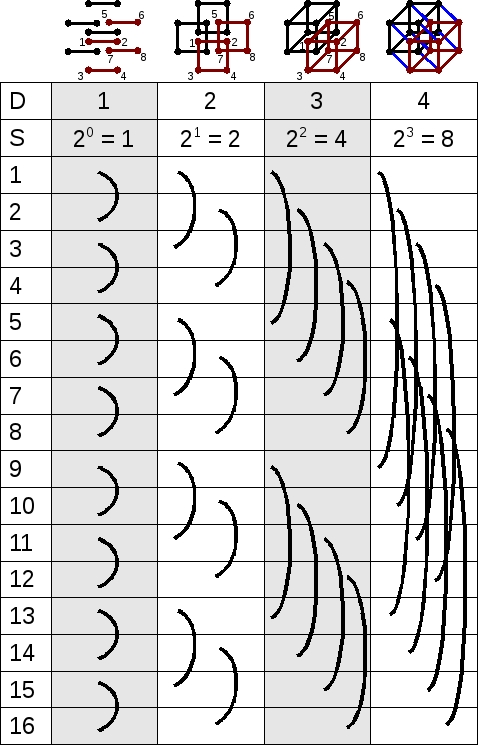
\includegraphics[width=0.5\linewidth]{images/theorie/hyper-build}
  \caption[Visuelle Darstellung des Algorithmus zur Erstellung eines Hypercube]{Darstellung des Algorithmus zur Erstellung eines Hypercube\index{Hypercube} der vierten Dimension. In jeder Dimension $D$ werden jeweils $S = 2^{D-1}$ Knoten nacheinander mit den $S$ n\"achsten Verbunden. Anschliessend werden $S$ Knoten \"ubersprungen und die noch ausstehenden wie vorhin verbunden. Codeblock \ref{alg:praxis-basis-hypercube-algemein} zeigt ein Code-Beispiel dieses Vorganges.}
  \label{fig:praxis-basis-hypercube}
\end{figure}

Zur Bildung eines Hypercube\index{Hypercube} muss zuerst die Dimension und die Anzahl Nodes bekannt sein. Die Dimension legt dabei fest, wie viele Verbindungen jede Node aufweist, also wie viele Schritte zur Berechnung notwendig sind. Bei einem Hypercube der dritten Dimension (ein W\"urfel) weist jede Node drei Verbindungen auf. Es sind also drei Durchg\"ange notwendig. Der Prozess f\"angt bei der ersten Node im ersten Durchgang an. Diese erste Node wird mit der nachfolgenden verbunden, also Node zwei. Da die zweite Node nun schon eine Verbindung aufweist, muss diese \"ubersprungen werden und mit der dritten weitergemacht werden. Diese wird anschliessend wiederum mit der nachfolgenden, also der vierten Node verbunden. Dieser Prozess wird so lange wiederholt bis alle Nodes eine Verbindung aufweisen.

Beim zweiten Durchlauf wird wieder mit der ersten Node angefangen, jedoch wird dieses mal nicht erneut eine Verbindung mit der zweiten Node hergestellt, sondern mit der Dritten. Die zweite Node besitzt noch keine zwei Verbindungen, also ist diese als n\"achste dran und wird mit der vierten Node verbunden. Node drei und vier weisen nun schon je zwei Verbindungen auf, es wird also mit der f\"unften Node weitergemacht und diese mit der Siebten verbunden. Nach dem zweiten Durchlauf weisen alle Nodes je zwei Verbindungen auf. Auf dem Papier w\"aren nun also zwei Quadrate zu sehen.

Diese beiden Quadrate m\"ussen im dritten Durchlauf nun zu einem W\"urfel zusammengesetzt werden, was wieder nach dem gleichen Prinzip geschieht. Begonnen wird wieder mit der ersten Node. Diese muss nun in die dritte Dimension verbunden werden, also mit der f\"unften Node. Die zweite Node muss eine Verbindung zur sechsten, die dritte eine zur siebten und die vierte eine zur achten Node aufbauen. Um die n\"achste Dimension zu verbinden, was dann die 4. Dimension w\"are, sind nicht mehr je vier Nodes zu verbinden und zu \"uberspringen, wie in der dritten, sondern je acht St\"uck.

Darauf aufbauend kann der Algorithmus in folgenden wenigen Aussagen zusammengefasst werden:
\begin{itemize}
 \item Im ersten Durchlauf wird jeder Knoten mit dem Nachfolgenden verbunden, wenn dieser nicht schon eine Verbindung aufweist. Es entstehen folgende Verkn\"upfungen: $1 \rightarrow 2$, $3 \rightarrow 4$, $5 \rightarrow 6$, $7 \rightarrow 8$, ...
 \item Im zweiten Durchlauf wird jeder Knoten mit dem \"ubern\"achsten verbunden, wenn dieser nicht schon eine Verbindung aufweist. Es entstehen folgende Verkn\"upfungen: $1 \rightarrow 3$, $2 \rightarrow 4$, $5 \rightarrow 7$, $6 \rightarrow 8$ ...
 \item Der dritte Durchlauf ist entsprechend, nur dass jeweils 3 Knoten ausgelassen werden. Die Verkn\"upfungen sind entsprechend: $1 \rightarrow 5$, $2 \rightarrow 6$, $3 \rightarrow 7$, $4 \rightarrow 8$ ...
 \item Im vierten Durchlauf werden dann nicht mehr 3 Knoten ausgelassen, sondern total sieben.
\end{itemize}
Pro Durchlauf m\"ussen also immer $2^{dimension-1}$ Nodes verbunden und anschliessend auch $2^{dimension-1}$ Nodes \"ubersprungen werden. Eine visuelle Darstellung des Prozesses ist in Abbildung \ref{fig:praxis-basis-hypercube} zu sehen. Aus der Grafik wird auch ersichtlich, dass die Spr\"unge pro Dimension jeweils um eine Zweierpotenz h\"oher sind.

\begin{figure}[h]
 \lstset{language=[ISO]C++}
 \begin{lstlisting}[label=alg:praxis-basis-hypercube-algemein,caption={[Algorithmus zur Erstellung eines Hypercubes]Algorithmus zur Erstellung eines Hypercubes\index{Hypercube} basierend auf einer Liste von Nodes. Die Pr\"ufung auf "`null"' bei der Verkn\"upfung behebt das Problem der leeren Knoten. Das Modulo mit der Anzahl existierender Knoten (Zeile 6) beim zu verbindenden Knoten gew\"ahrleistet, dass keine "`null"'-Node \"ubergeben wird und dass jede Node mehr als nur eine Verbindung aufweist.}]
for (dim = 0; dim < dimension; dim++) {
  dim_2 = Math.pow(2, dim);
  for (i = 0; i < num_nodes; i += (2*dim_2)) {
    for (j = 0; j < dim_2; j++)  {
      if (node_list[i+j] != null) {
        _n = (i + j + dim_2) % num_real_nodes;
        node_list[i + j].connectNode(list[_n]);
      }
    }
  }
}
 \end{lstlisting}
\end{figure}

Dieser Algorithmus kann in dieser Form einfach und schonend in ein Programm umgesetzt werden. Ein Beispiel zeigt Codeblock \ref{alg:praxis-basis-hypercube-algemein}, wobei bei dieser Implementierung zus\"atzlich noch leere Knoten ber\"ucksichtigt werden. Es wird davon ausgegangen, dass bei der Verbindung der Knoten durch die Funktion \texttt{connectNode(node)} geschaut wird, ob der \"ubergebene Knoten bereits eine Verbindung mit dem zu verbindenden Knoten aufweist oder nicht. Nur wenn noch keine Verbindung besteht, wird eine hergestellt (siehe Codeblock \ref{alg:praxis-basis-hypercube-connect}). W\"urde dies nicht gepr\"uft, k\"onnte ein Knoten mehrfach mit dem gleichen Knoten verbunden werden und es m\"usste mittels einem zus\"atzlichen Parameter definiert werden, ob der aktuelle Aufruf aus dem Algorithmus oder aus der Funktion kommt. Nur wenn der Aufruf direkt vom Algorithmus gemacht w\"urde, d\"urfte der \"ubergebene Knoten mit dem aktuellen verbunden werden (Zeile 12). Ansonsten w\"urden sich die Verbindungsfunktionen auf den zwei Knoten endlos gegenseitig aufrufen.

\begin{figure}[h]
 \lstset{language=[ISO]C++}
 \begin{lstlisting}[label=alg:praxis-basis-hypercube-connect,caption={[Verbinden von zwei Hypercube-Nodes]Die Funktion, welche zwei Knoten verbindet, pr\"uft zuerst ob der Knoten nicht schon in der Liste vorhanden ist. Wenn nicht, wird der Knoten eingef\"ugt und die gleiche Funktion auf dem zu verbindenden Knoten aufgerufen. Ohne diese Pr\"ufung w\"urde hier eine endlose Aufruf-Aktion stattfinden.}]
if (node == null) return;
if (node == this) return;
bool connected = false;
foreach (HyperNode c_node in node_list) {
  if (c_node == node) {
    connected = true;
    break;
  }
}
if (!connected) {
  node_list.append(node);
  node.connectNode(this);
}
 \end{lstlisting}
\end{figure}

\subsection{Versenden von Alert-Nachrichten} \label{sec:praxis-basis-sendalert}
Das Problem der mehrfachen Meldungs-Zustellung wurde bereits in Kapitel \ref{sec:theorie-alert} diskutiert und dazu eine akzeptable L\"osung gefunden. Das System schaut in einem ersten Schritt in der Datenbank nach, wann dieser Alert (basierend auf Host und Modul) zuletzt gesendet worden ist. Anhand des Zeitstempels sowie des Pr\"ufintervals wird dann entscheiden, ob die aktuelle Meldung notwendig ist oder nicht.

Die Benachrichtigung, welches Modul bei welchem System fehlgeschlagen ist, wird durch den \texttt{MainListener} empfangen und durch das \texttt{MainSystem} in die Datenbank eingetragen. Die Alert-Funktion \texttt{sendAlert} liest diese Daten aus und entscheidet, ob eine Meldung versendet werden soll. Soll ein Alert versendet werden, wird dies zuerst den anderen \"Uberwachungssystemen mitgeteilt und anschliessend die Alert-Meldung versendet. In Abbildung \ref{fig:alert-sample} wird zuerst die Meldung versendet und anschliessend die anderen Systeme dar\"uber informiert. Dies kann jedoch dazu f\"uhren, dass eine Meldung mehrfach versendet wird, denn w\"ahrend das eine System eine Nachricht sendet, k\"onnen andere den Ausfall ebenfalls bemerken und eine Meldung versenden.

Grunds\"atzlich w\"urde eine Meldung unter Umst\"anden alle paar Sekunden versendet werden, denn bei der ausgearbeiteten L\"osung wird nur basierend auf dem Pr\"ufungsintervall eine Pause definiert. Um diesem Problem Herr zu werden, wird versucht heraus zu finden, wie lange das System bereits nicht mehr auf den Dienst reagiert. Basierend auf dieser Anzahl Sekunden kann anschliessend ein Alert-Plan geladen werden.

Ein Alert-Plan, definiert durch die \texttt{AlertConfig}-Klasse, beschreibt, wie mit einem Ausfall bei einem Modul und System sowie der entsprechenden Downtime umgegangen werden soll. Die Konfiguration beinhaltet den Namen des \"Uberwachungsmodules, die Sekundenwerte "`von"' und "`bis"' zur Definierung der Downtime, ein Timeout in Sekunden sowie eine Liste von Empf\"angern. Basierend auf dem Timeout und der letzten Alert-Meldung kann somit gesagt werden, ob oder wann eine Meldung versendet werden soll.

In der f\"ur die Bachelor-Thesis ausgearbeiteten Technologie-Demonstration wird der Alert-Plan eine statische Liste von Werten sein. In einer zuk\"unftigen Version wird diese global pro Dienst definiert und auf Systemebene noch verfeinert werden k\"onnen. Es kann zuk\"unftig somit bestimmt werden, welcher Dienst \"uber welches Alert-Modul bei welchen Personen eine Benachrichtigung hinterlassen soll.


%%%%%%%%%%%%%%%%%%%%%%%%%%%%%%%%%%%%%%%%%%%%%%%%%%%%%%%%%%%%%%%%%%%%%%%%%%%%%%%%%%%%%%%%%%%%%%%%%%%%%%%%%%%%%%%%%%%%%%%%%%%%%%%%%%%%%%%%%
\section{Einfache Installation und Konfiguration} \label{sec:praxis-install}
In einer finalen Version sollte das Produkt nicht nur als bin\"are Version, sondern auch als Quellcode verf\"ugbar sein. Die Voraussetzung f\"ur die Compilierung ist nicht nur ein aktueller Vala- sondern auch ein C-Compiler. Zus\"atzlich m\"ussen noch verschiedene Libraries wie die GLib, GEE und GIO vorhanden sein, sowie Datenbank-Bibliotheken f\"ur die verschiedenen Module. Sind alle Voraussetzungen gegeben, kann der Quellcode durch GNU-Make kompiliert und anschliessend verwendet werden.

Ist das Produkt in einer bin\"aren Form vorhanden, muss dieses nur in einen Ordner kopiert und kann dort direkt gestartet werden. Die Grundkonfiguration, also welche Datenbank-Engine genutzt werden soll, kann \"uber einen Startparameter definiert werden. Andere Einstellungen m\"ussen nicht get\"atigt werden. Damit das Programm beim Systemstart automatisch gestartet wird, muss nur noch ein entsprechendes Kommando in den Startprozess eingef\"ugt werden. Dieser ist nicht nur plattformabh\"angig sondern auch unter Linux/BSD/Unix unterschiedlich von Distribution zu Distribution.

Um ein System in die \"Uberwachung mit auf zu nehmen, muss dieses \"uber eine Weboberfl\"ache oder ein anderes Remote-API-Modul konfiguriert werden. Diese Grundkonfiguration kann dabei auf zwei unterschiedliche Arten erfolgen:

\begin{description}
 \item[\"Uber eine direkte Verbindung] kann dem neuen System mitgeteilt werden, welche IP-Adresse es hat und in welchem Netzwerk es ist. Soll das System in ein bestehendes \"Uberwachungsnetzwerk eingebunden werden, muss dem neuen System nur ein anderes im gleichen Netzwerk vorhandenes System angegeben werden. Ist in dem neuen Netzwerk kein anderes System vorhanden, m\"ussen eventuelle weitere Parameter angegeben werden, um zum Beispiel eine OpenVPN-Verbindung\index{VPN!OpenVPN} aufbauen zu k\"onnen.

 \item[\"Uber ein anderes System] kann das neue System ebenfalls eingebunden werden. Auf einem System kann \"uber ein Remote-API-Modul ein neues System durch die Angabe von IP-Adresse und Netzwerk eingebunden werden. Diese Methode funktioniert jedoch nicht, wenn das neue System das einzige in einem neuen Netzwerk ist, denn dieses besitzt noch keine OpenVPN-Daten und Verbindungen.
\end{description}

Ist das neue System erst einmal im Netzwerk registriert, kann die Konfiguration an diesem vorgenommen werden. Durch einfache Prozessabl\"aufe k\"onnen verschiedene Dienste konfiguriert werden. Sind alle Parameter und Dienste eines Systems konfiguriert, kann durch eine Synchronisation das entsprechende System aktualisiert werden. Eine solche Synchronisation sollte jedoch erst nach Beendigung der Konfiguration durchgef\"uhrt werden, denn durch eine Einbindung eines neuen Systems oder Dienstes, wird eine komplette Neubildung des Hypercubes f\"allig.

Die grundlegenden Konfigurationen wie die globalen und lokale Datenbanken, VPN-Daten etc. werden ebenfalls mittels den Remote-API-Modulen konfiguriert. Bei der Synchronisation von diesen wird aber in den meisten F\"allen kein Rebuild des Hypercubes notwendig. Eine Reinitialisierung des Management-Netzwerkes oder des Systems ist m\"oglich.

\subsection{M\"ogliche Funktionen einer Konfigurationsoberfl\"ache} \label{sec:praxis-install-conf}
Eine Konfigurationsoberfl\"ache sollte wenn m\"oglich die nachfolgenden Funktionen und Bereiche aufweisen:

\begin{description}
 \item[Grundkonfiguration:] Die Grundkonfiguration beinhaltet alle Basis-Parameter und Definitionen. Dies sind zum Beispiel globale Parameter der einzelnen \"Uberwachungsmodule wie ein Timeout bei einem ECHO-Request, welche Datenbank als Standard verwendet wird, ob und welche Datenbank als globaler Datenbank-Mirror/Backbone verwendet wird, etc.

 \item[Netzwerke:] Die Netzwerk-Konfiguration definiert in erster Linie das Netzwerk anhand einer IP-Adresse und einer Subnet-Maske. Zus\"atzlich werden noch Parameter f\"ur die Herstellung eines OpenVPN-Management-Netzwerkes\index{VPN!OpenVPN} sowie eine Gateway-Adresse definiert, \"uber welche die anderen Netzwerke kommunizieren k\"onnen.

 \item[Network-Discovery:] Das Network- oder auch Host-Discovery dient in erster Linie dazu, neue Systeme in einem Netzwerk zu finden und diese zu untersuchen. Die so gefundenen Systeme k\"onnen anschliessend \"uber die \textbf{Host-Konfiguration} bearbeitet werden.

 \item[Host-Konfiguration:] Dieser Bereich listet alle Systeme und deren \"uberwachten Dienste auf. Auf den einzelnen Systemen k\"onnen neue Dienste hinzugef\"ugt, entfernt oder bearbeitet werden. Die globale System-Konfiguration wie IP-Adresse, Netzwerk, usw. sollte ebenfalls dar\"uber konfigurierbar sein.
\end{description}

\subsection{Installation der TechDemo} \label{sec:praxis-install-demo}
Die Technologie-Demonstration soll die Machbarkeit aufzeigen und nicht ein voll funktionst\"uchtiges Produkt darstellen. Zur Pr\"ufung der Funktionalit\"at werden relativ viele Informationen auf der Konsole ausgegeben.

Die Technologie-Demonstration erfordert aktuell mehr Konfigurationsaufwand als die geplante finale Version. Dazu notwendig ist ein Sqlite3-Datenbank-Programm wie SQLiteMan (\url{http://www.sqliteman.com/}) um verschiedene Systeme in die \"Uberwachung auf zu nehmen. Die TechDemo wird in zwei Bin\"ar-Versionen angeboten (32-Bit POSIX, 64-Bit POSIX) sowie auch als Vala-Sourcecode. Eine Windows-Version ist aktuell nicht vorhanden.

Die bin\"aren Versionen k\"onnen aus einem beliebigen Verzeichnis gestartet werden. Als Startparameter werden die IP-Adresse als Dot-String sowie die Subnet-Maske als numerischer Wert ben\"otigt: \texttt{./modules 1.2.3.4 24}

Vor dem ersten Start sollte die Datei "`dummy\_alert\_config.txt"' im data-Ordner bearbeitet werden. Diese beinhaltet momentan die Konfiguration f\"ur das EMail-Alert-Modul. Die Parameter sollten selbstbeschreibend sein, eine Auflistung und Beschreibung ist aber im Anhang in Tabelle \ref{tbl:praxis-install-dummyalertconf} zu sehen. Anschliessend muss die Sqlite-Datenbank "`config.sqlite"', ebenfalls im data-Verzeichnis, bearbeitet werden. In der Tabelle "`networks"' muss in einem ersten Schritt das bestehende Netzwerk angepasst und allenfalls zus\"atzliche eingetragen werden. In der Tabelle "`hosts"' m\"ussen alle anderen \"Uberwachungssysteme eingetragen werden. Die Tabelle "`modules"' schlussendlich beinhaltet alle Systeme, welche \"uberwacht werden sollen. Jede Zeile in der "`modules"' Tabelle steht f\"ur einen Parameter. Es werden somit zwei Zeilen ben\"otigt, wenn ein System mittels \texttt{icmp} alle 5 Sekunden (timeout) und je 2 Echo-Requests (num) \"uberwacht werden soll.

Sind alle Konfigurationen gemacht, kann das System, wie oben angegeben, gestartet werden. Kommandos k\"onnen anschliessend mittels "`netcat"' (siehe Kapitel \ref{sec:praxis-basis-kernel-listener}) dem System \"ubergeben werden. Mit der Erstellung von Test-Hosts sollte vorsichtig umgegangen werden. Da Sqlite nicht gerade die schnellste Datenbank ist, kann zum Beispiel die Erstellung eines /16-er Netzwerkes mit mehreren tausend Systemen einige Minuten in Anspruch nehmen.

Alternativ kann auch mittels einem aktuellen Firefox oder einem auf KHTML/WebKit basierenden Browser wie Chrome oder Safari eine Konfiguration \"uber das JSON-RPC-Modul vorgenommen oder ge\"andert werden. Hierf\"ur muss die die Datei "`json-rpc.html"' aus dem "`demo"'-Verzeichnis ge\"offnet werden. Der erste Dialog dient zur Angabe eines laufenden Systems, wobei als Standard-Port f\"ur JSON-RPC momentan der Port 2784 (www-dev) verwendet wird. Die Oberfl\"ache dieser Demo-Weboberfl\"ache sollte weitgehenst selbsterkl\"arend sein: Im linken Bereich werden alle Netzwerke und durch einen Klick auf ein solches auch die Systeme angezeigt. Durch einen klick auf ein System werden mittig die System-Konfigurationen dargestellt und rechts ein Kommunikations-Log. Oberhalb wird eine Menubar/Symbolleiste angezeigt, \"uber welche verschiedene Aktionen ausgef\"uhrt werden k\"onnen. Wichtig bei der Ben\"utzung zu wissen ist, dass der Server teilweise keine Verbindungen annimmt, was zu Fehlern f\"uhren kann. Wird ein solcher Fehler gezeigt muss unter umst\"anden die Seite neu geladen werden, da die Browser erst anschliessend wieder in der Lage sind eine Verbindung herzustellen.

Ein Problem bei der aktuellen Version stellt ein Speicherfehler in der SQLite3-Bibliothek dar. Bei der Verwendung von \texttt{Sqlite3.Statement} beim auslesen von Daten, werden Speicherbereiche nicht mehr korrekt fereigegeben. Dies hat zur Folge dass durch den Betrieb der \"Uberwachungs-Software aktuell immer mehr Speicher (heap) verbraucht wird und nicht wiederverwendet werden kann. Durch die Verwendung von Sqlite3 als externe Bibliothek, kann es durchaus sein, dass dieser Fehler nicht auf jeder Installation vorhanden ist.

\section{Verschiedene Szenarien} \label{sec:praxis-businesscases}
Zur Veranschaulichung der Technologie-Demonstration werden in diesem Kapitel einige Szenarien nachgespielt sowie die Reaktion des Systems darauf gezeigt.

\subsection{Rebuild eines Hypercubes}
Damit der Prozess der Bildung eines Hypercube besser gezeigt werden kann, wird eine Datenbank mit 20 Pseudo-Systemen aus dem Subnet "`192.168.22.0/24"' verwendet. Diese Dummy-Hosts werden durch den Befehl \texttt{echo '1   1   a8812636a6ad0b84ab8f6943728551a4""testdata: 192.""168.""22.0 24 20' \textbar nc -q1 -u 192.""168.""22.""27 1611} angelegt und durch \texttt{echo '1   1   a8812636a6ad0b84ab8f6943728551a4""rebuild:' \textbar nc -q1 -u 192.""168.""22.""27 1611} neu gebildet.

\begin{figure}[H]
  \centering
  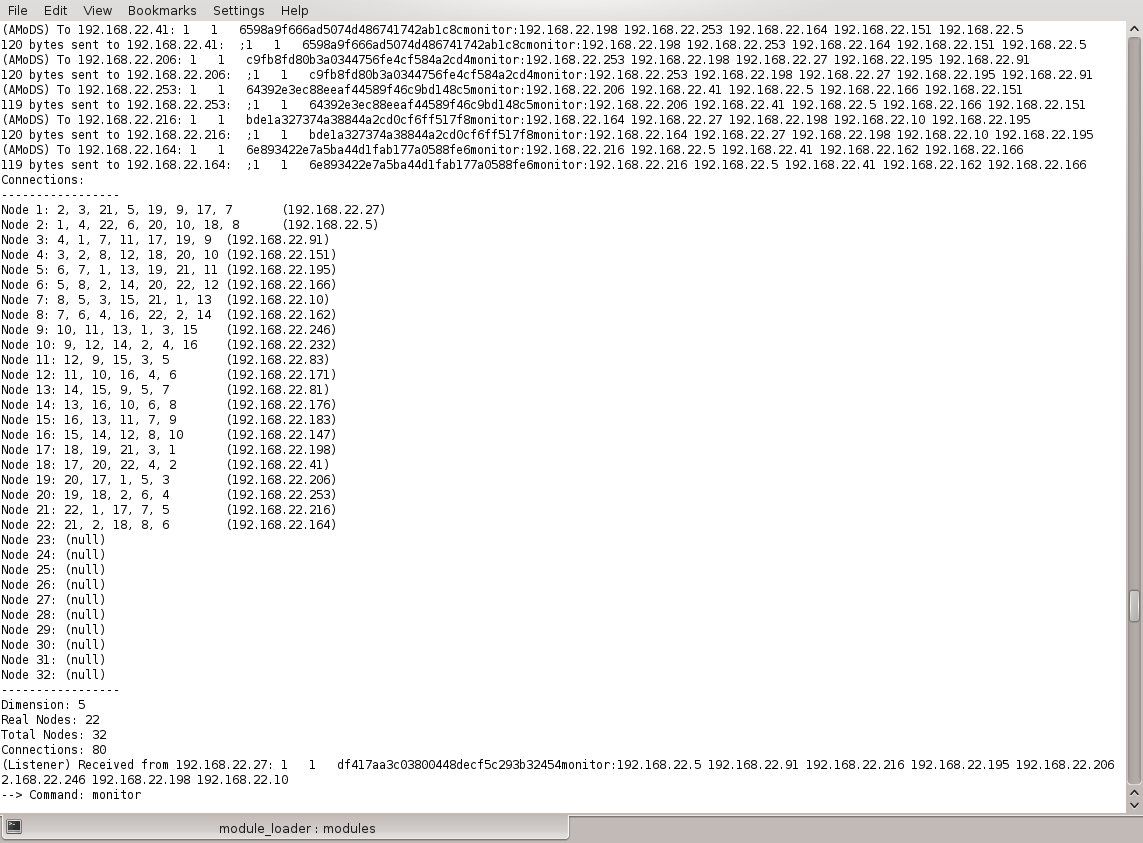
\includegraphics[width=0.9\linewidth]{images/theorie/amods_rebuild}
  \caption[Erstellen von DummyHosts und Rebuild des Hypercubes]{Im oberen Bereich sind Nachrichten sichtbar, welche die anderen Systeme dar\"uber informieren, welche anderen Systeme sie \"uberwachen m\"ussen. Der mittlere Bereich zeigt den Hypercube, respektive alle gemachten Verbindungen zwischen den Systemen. Unten angef\"ugt werden noch die Hypercube-Daten gezeigt. Die letzten Zeilen zeigen die eingegangene Nachricht, welche dem aktuellen System mitteilt, welche anderen Systeme es \"uberwachen muss.}
  \label{fig:nat-source}
\end{figure}

\textbf{Achtung:} Wenn Systeme manuell in die Datenbank eingetragen worden sind, die nicht im gleichen Netzwerk wie der aktuelle Server sind, werden diese aus der \"Uberwachung entfernt. Es wird nicht das System an sich entfernt, sondern nur die Eintr\"age in der "`modules"'-Tabelle, welche alle \"uberwachten Systeme beinhaltet.

\subsection{Ausfall eines Systems}
F\"allt ein System aus und wird ein Alert versendet, wird dies allen anderen Systemen mitgeteilt. Zus\"atzlich ist in diesem Szenario noch ein Konfigurationsfehler, welcher das senden einer Alert-Meldung nicht zul\"asst. Dieser Fall wird in der TechDemo jedoch nicht abgefangen, denn es wird grunds\"atzlich davon ausgegangen, dass ein Alert versendet werden kann.

\begin{figure}[H]
  \centering
  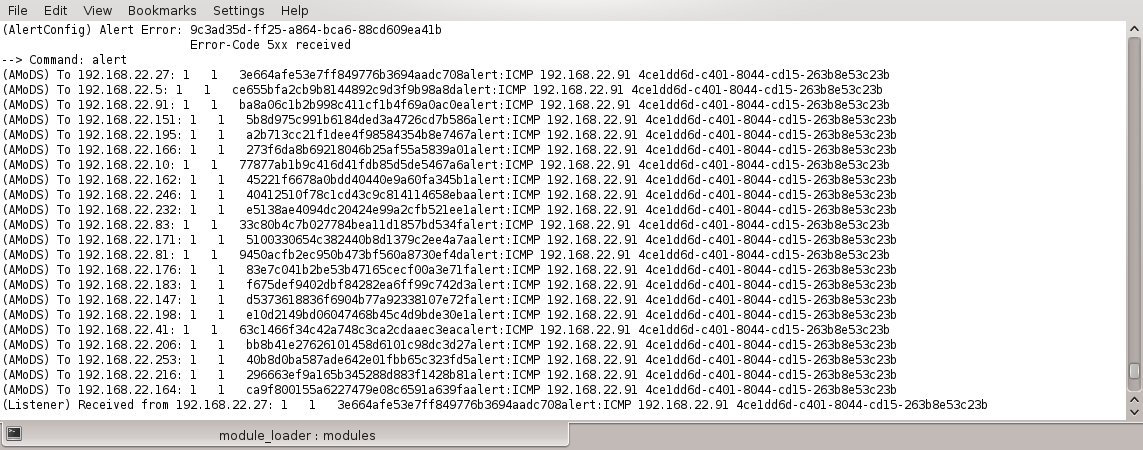
\includegraphics[width=0.9\linewidth]{images/theorie/amods_ausfall}
  \caption[Ausfall eines Systems]{Die ersten Zeilen zeigen auf, dass der Alert nicht versendet werden konnte. Der EMail-Server hat einen 5xx-Code als Antwort gesendet. Die anschliessenden Zeilen zeigen die Nachrichten an alle weiteren Systeme, welche informiert werden, dass der Alert mit der ID \textbf{4ce1dd6d-c4...} f\"ur das System \textbf{192.168.22.91} und Plugin \textbf{ICMP} versendet worden ist. Die letzte Zeile zeigt auf, dass das laufende System die oben gesendete Nachricht auch empf\"angt und weiterverarbeitet.}
  \label{fig:nat-source}
\end{figure}

Wird ein Systemfehler entdeckt, ein Alert wurde jedoch schon gesendet, wird so lange gewartet, bis wieder ein Alert versendet werden darf.

\begin{figure}[H]
  \centering
  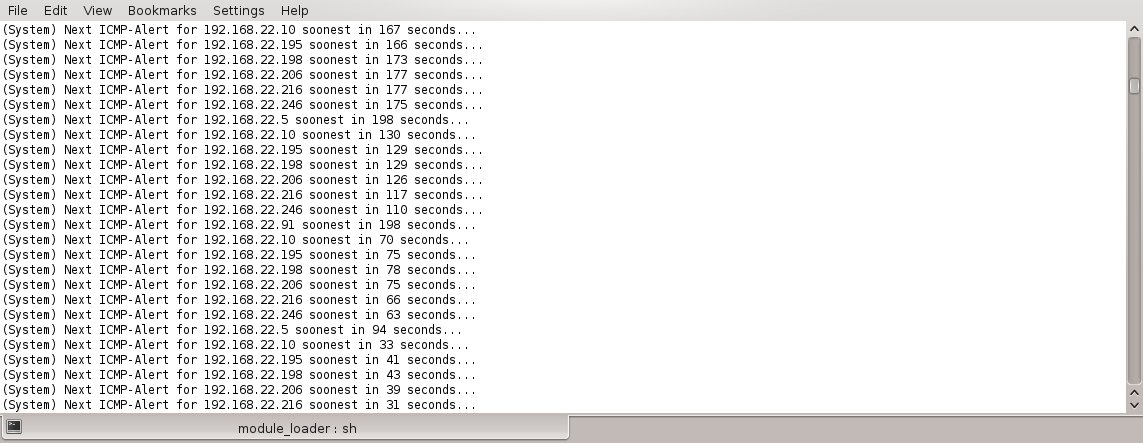
\includegraphics[width=0.9\linewidth]{images/theorie/amods_waiting}
  \caption[Warten beim Ausfall eines Systems]{Wird das Senden eines Alerts beim auffinden eines Problems durch eine Semaphore geblockt, wird dies aktuell durch die Wartezeit angezeigt.}
  \label{fig:nat-source}
\end{figure}


\subsection{\"Uberwachung eines EMail-Servers}
Wird bei der SMTP-Modul-Konfiguration ein Fehler gemacht, wird dies aktuell nicht erkannt, sondern es wird angenommen, dass etwas mit dem System nicht in Ordnung ist.

\begin{figure}[H]
  \centering
  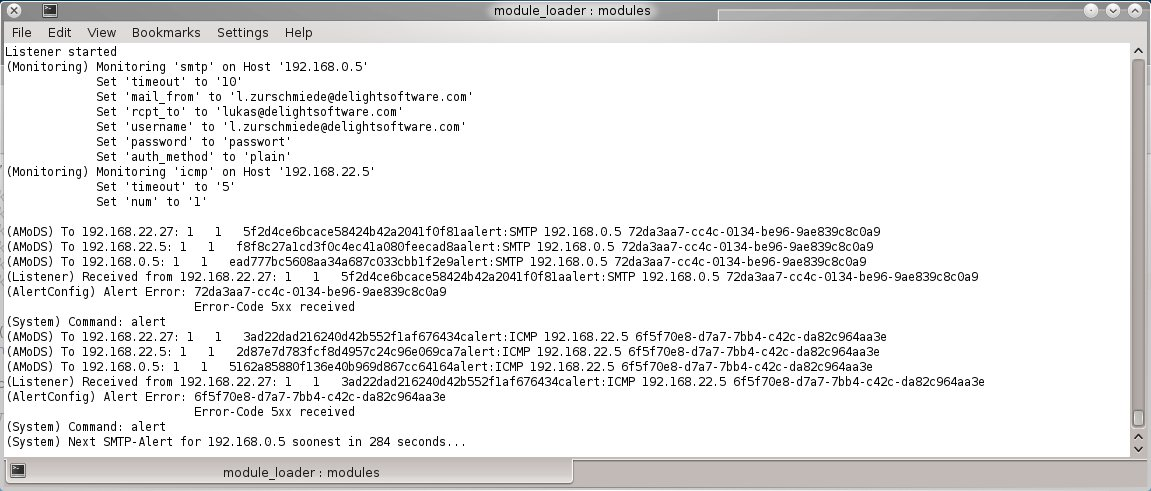
\includegraphics[width=0.9\linewidth]{images/theorie/amods_email_error}
  \caption[Fehler beim \"uberwachen eines EMail-Servers]{Auf den ersten Zeilen wird gezeigt, mit welchen Parametern das SMTP-Modul geladen wird. Das fehlerhaft Passwort verursacht eine Alert-Meldung, welche anschliessend auf die umliegenden Systeme verteilt wird.}
  \label{fig:nat-source}
\end{figure}





\chapter{Fazit} \label{sec:fazit}

Es existieren viele gute und zuverl\"assige Softwarel\"osungen zur \"Uberwachung von Systemen und Netzwerken auf dem Markt. Die meisten, wenn nicht sogar alle, bauen auf dem Prinzip der zentralen Datenerfassung auf. Alle Systeme werden von einem zentralen Punkt aus \"uberwacht. Nachrichten und Meldungen werden von dieser zentralen Instanz gespeichert und versendet. Einige Systeme arbeiten mit zus\"atzlichen Satelliten oder Agents, welche die Aufgabe haben, gewisse Netzwerksegmente zu \"uberwachen. Diese dezentralen Instanzen sind jedoch nichts anderes als Proxys, also Schnittstellen, welche Dienste pr\"ufen k\"onnen und die Resultate an die zentrale Einheit weiterleiten.

Die Idee einer hochverf\"ugbaren und autonomen \"Uberwachung m\"usste, basierend auf diesen Fakten, eigentlich schon zu einem fr\"uheren Zeitpunkt aufgekommen sein. Bei jedem Server-Ausfall, Netzwerkzusammenbruch oder sonstigem Problem mit der zentralen Instanz wird das komplette Netzwerk nicht \"uberwacht. Bei den Recherchen zu dieser Arbeit wurden weder Dokumente noch Abhandlungen oder Anderes gefunden, welche auf diese Idee hingewiesen oder dies sogar als Thema hatten.

Das Prinzip ist relativ einfach und schnell erkl\"art. Bei der theoretischen Betrachtung und der praktischen Umsetzung wurden jedoch vier kleinere Knackpunkte erkannt:
\begin{itemize}
 \item Die \"Uberwachung muss Netzwerk-\"ubergreifend sein, ohne \"uberm\"assige Router- und Firewall-Konfiguration.
 \item Wie werden die Systeme innerhalb eines Netzwerkes und wie die Netzwerke selbst automatisch verbunden und verkn\"upft?
 \item Ein Alert darf nur einmal und nicht von allen Systemen versendet werden.
 \item Es muss eine M\"oglichkeit geben, die Daten trotzdem zentral speichern zu k\"onnen.
\end{itemize}

Durch einen Hinweis von Herr Frank Moehle, dass die zu \"uberwachenden Systeme eventuell nach dem Prinzip eines Hypercube miteinander verh\"angt werden k\"onnten, stellte sich schnell heraus, dass die ersten zwei Probleme in der Theorie relativ einfach zu l\"osen sind: Die Systeme eines jeden Netzwerkes bilden einen Hypercube. Die Netzwerke bilden ebenfalls einen. Dadurch beh\"alt man nicht nur die Anzahl an Verbindungen im Griff, sondern die Systeme k\"onnen auch automatisch fragmentiert und die Verbindungen der verschiedenen Netzwerke einfach konfiguriert werden.

Die Tatsache, dass viele Server und auch Netzwerkkomponenten heutzutage \"uber eine Management-NIC verf\"ugen, vereinfacht das erste Problem weiter. Durch die Kommunikation \"uber dieses Netzwerk-Interface k\"onnen Router und Firewalls genereller konfiguriert werden. Da jedoch nicht alle Rechner und Komponenten \"uber zwei Netzwerkkarten verf\"ugen, muss die M\"oglichkeit bestehen, dass die Kommunikation dennoch \"uber einen separaten Kanal erfolgen kann. Dies kann durch die optionale Vernetzung der Systeme durch OpenVPN erfolgen.

Die einzige Schwierigkeit ergab sich anschliessend in der praktischen Umsetzung bei der Herleitung des Algorithmus zur automatischen Bildung eines Hypercubes. Dar\"uber wurden leider weder Informationen noch Hinweise noch Anregungen gefunden. Dies bedeutete, dass dieser Algorithmus selber hergeleitet, vereinfacht und vor allem speicherschonend ausgearbeitet werden musste. Dies war eine der interessantesten Aufgaben der gesamten Thesis.

Die Problematik zur Verhinderung des mehrfachen Sendens von Alert-Nachrichten konnte durch relativ einfache Pr\"ufungen und Notifikationen behoben werden.

Die zentrale Datenspeicherung aller Pr\"ufergebnisse und Nachrichten konnte ebenfalls einfach gel\"ost werden. Alle Daten, die zentral gespeichert werden sollen, m\"ussen einfach durch alle konfigurierten Daten-Module gespeichert werden. Dabei spielt es f\"ur die Software keine Rolle, wo und wann welche Daten gespeichert werden. W\"ahrend das eine Modul alle Daten in einer lokalen Sqlite3-Datenbank speichert, schickt ein zweites Modul alle Daten zus\"atzlich noch in einen MySQL-Cluster oder \"uber eine definierte Schnittstelle an ein beliebiges anderes System.

Die Frage, warum bislang noch kein solches System existiert, kann nach der Bachelor-Thesis immer noch nicht beantwortet werden. Die Probleme, welche sich bei der Planung und der praktischen Ausarbeitung ergeben haben, unterscheiden sich nicht von denen bei anderen Software-Projekten. Die Vorteile, die ein solches System bietet, \"ubertreffen meiner Meinung nach die Vorteile zentralisierter Systeme. Dabei ist nicht nur die Hochverf\"ugbarkeit ein Pluspunkt sondern auch die verteilte Netzwerklast, welche bei einem zentralisierten System ebenfalls zentralisiert ist.





%% Anhang etc.
\newpage
\setcounter{page}{1}
\pagenumbering{Alph}

%% Abk\"urzungsverzeichnis
\abbrev[prefix]{IP}{Internet Protocol}
\abbrev[prefix]{VPN}{Virtual Private Network}
\abbrev[prefix]{SSL}{Secure Socket Layer}
\abbrev[prefix]{SSL-VPN}{Secure Socket Layer Virtual Private Network}
\abbrev[prefix]{MID}{Man in the Middle}
\abbrev[prefix]{XSS}{Cross-Site Scripting}
\abbrev[prefix]{DPI}{Deep Packet Inspection}
\abbrev[prefix]{IPS}{Intrusion Prevention System}
\abbrev[prefix]{ARP}{Address Resolution Protocol}
\abbrev[prefix]{MAC}{Media Access Control, Hardwareadresse (Dt)}
\abbrev[prefix]{SNMP}{Simple Network Management Protocol}
\abbrev[prefix]{MIB}{Management Information Base}
\abbrev[prefix]{MO}{Managed Object}
\abbrev[prefix]{OID}{Object Identifier}
\abbrev[prefix]{PDU}{Protocol Data Unit}
\abbrev[prefix]{IPMI}{Intelligent Platform Management Interface}
\abbrev[prefix]{BMC}{Baseboard Management Controller}
\abbrev[prefix]{SMBus}{System Management Bus}
\abbrev[prefix]{RBL}{Realtime Blacklist}
\abbrev[prefix]{SMS}{Short Message Service}
\abbrev[prefix]{MMS}{Multimedia Message Service}
\abbrev[prefix]{GSM}{Global System for Mobile Communications}
\abbrev[prefix]{FME}{Funk-Melde Empf\"anger}
\abbrev[prefix]{DME}{Digitale Melde Empf\"anger}
\abbrev[prefix]{POCSAG}{Post Office Code Standard Advisory Group}
\abbrev[prefix]{TETRA}{Terrestrial Trunked Radio}
\abbrev[prefix]{API}{Application Programming Interface}
\abbrev[prefix]{SMTP}{Simple Mail Transport Protocol}
\abbrev[prefix]{AMoDS}{Autonomous Monitoring of Distributed Services}
\abbrev[prefix]{NIC}{Network Interface Card}
\abbrev[prefix]{TCP}{Transmission Control Protocol}
\abbrev[prefix]{IP}{Internet Protocol}
\abbrev[prefix]{IPv4}{Internet Protocol version 4}
\abbrev[prefix]{IPv6}{Internet Protocol version 6}
\abbrev[prefix]{ISP}{Internet Service Provider}
\abbrev[prefix]{UDP}{User Datagram Prodocol}
\abbrev[prefix]{MX}{Mail Exchange}
\abbrev[prefix]{NRPE}{Nagios Remote Plugin Executor}
\abbrev[prefix]{IIS}{Intrnet Information Server, Microsoft Webserver}
\abbrev[prefix]{SQL}{Structured Query Language}
\abbrev[prefix]{RRD}{Round Robin Database}
\abbrev[prefix]{CDP}{Cisco Discovery Protocol}
\abbrev[prefix]{LLDP}{Link Layer Discovery Protocol}
\abbrev[prefix]{NAT}{Network Address Translation}
\abbrev[prefix]{HTTP}{Hyper Text Transfer Protocol}
\abbrev[prefix]{SMTP}{Simple Mail Transfer Protocol}
\abbrev[prefix]{POP3}{Post Office Protocol v.3}
\abbrev[prefix]{IMAP}{Internet Message Access Protocol}
\abbrev[prefix]{ICMP}{Internet Control Message Protocol}
\abbrev[prefix]{FTP}{File Transfer Protocol}
\abbrev[prefix]{FIFO}{First in first out}

\addcontentsline{toc}{chapter}{Abk\"urzungsverzeichnis}
\printglossary

% Index
%\newpage
%\addcontentsline{toc}{chapter}{Stichwortverzeichnis}
%\printindex

%% Abbildungs und Tabellenverzeichnis
\newpage
\addcontentsline {toc}{chapter}{Abbildungsverzeichnis}
\listoffigures
\addcontentsline {toc}{chapter}{Tabellenverzeichnis}
\listoftables
\addcontentsline {toc}{chapter}{Codeverzeichnis}
%\listofalgorithms
\lstlistoflistings

%% Literaturverzeichniss
\newpage
\addcontentsline {toc}{chapter}{Literaturverzeichnis}
\bibliography{literatur_concat}

%% Anhang
\newpage
\addcontentsline{toc}{chapter}{Anhang}
\chapter*{Anhang}

%% NAT Visualisierungen
\begin{figure}[H]
  \centering
  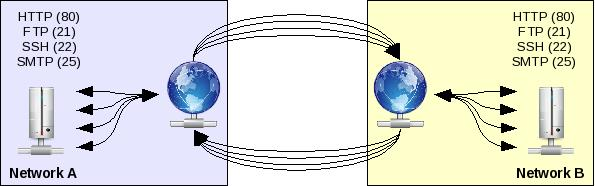
\includegraphics[width=0.6\linewidth]{images/theorie/nat-source}
  \caption[Anzahl NAT-Regeln bei zwei Netzwerken]{Beispiel f\"ur die Anzahl NAT-Regeln bei zwei Netzwerken mit jeweils einem Host, welche je vier Dienste \"uberwacht haben wollen. Beide NAT-Firewalls m\"ussen je vier Regeln definiert haben, um die Anfragen durch zu leiten.}
  \label{fig:nat-source}
\end{figure}

\begin{figure}[H]
  \centering
  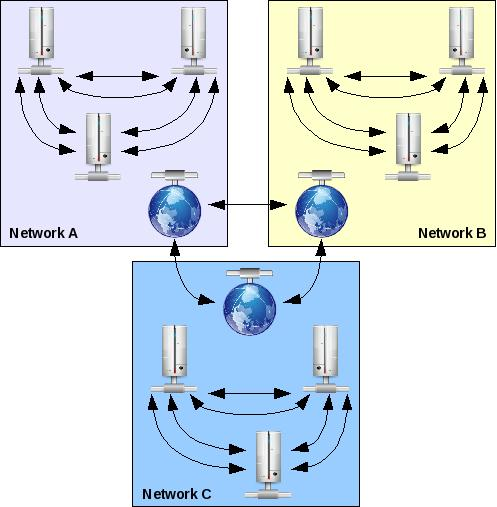
\includegraphics[width=0.6\linewidth]{images/theorie/nat-verteilt}
  \caption[Anzahl NAT-Regeln bei einer verteilten \"Uberwachung]{Beispiel f\"ur die Anzahl NAT-Regeln bei einer verteilten \"Uberwachung. Die NAT-Boxen m\"ussen jeweils nur eine Regel pro entferntem Netzwerk definiert haben, da dieses als Ganzes \"uberwacht wird und nicht jedes System einzeln.}
  \label{fig:nat-verteilt}
\end{figure}


%% Hypercube Visualisierungen
\begin{figure}[H]
  \centering
  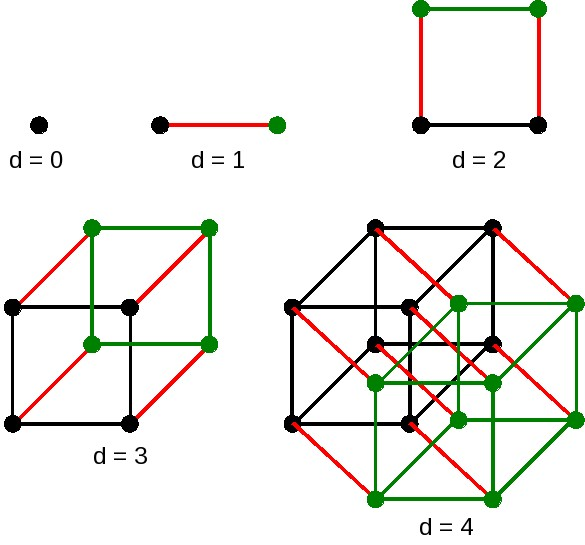
\includegraphics[width=0.6\linewidth]{images/theorie/hyper-sample}
  \caption[Hypercubes von Dimension 0 bis 4]{Hypercubes von Dimension $d=0$ bis $d=4$. Die Erstellung geschieht jeweils durch eine Verschiebung (gr\"un) des vorherigen Hypercubes in eine neue Dimension sowie dem Verbinden (rot) der jeweils gleichen Eckpunkte miteinander.}
  \label{fig:hyper-sample}
\end{figure}

\begin{figure}[H]
  \centering
  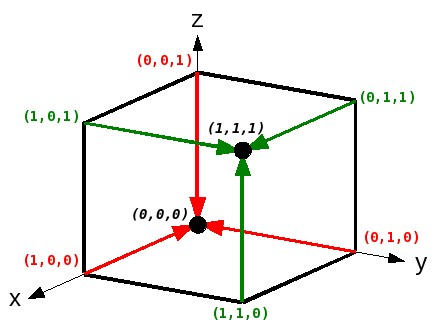
\includegraphics[width=0.6\linewidth]{images/theorie/hyper-hamming-4}
  \caption[Hamming-Distanz bei einem Hypercube zur Nummerierung der Nodes]{Die Nummerierung mit der Hamming-Distanz geschieht bei einem W\"urfel durch die Zuweisung der Werte $(0,0,0)$ und $(1,1,1)$ auf zwei gegen\"uberliegenden Ecken und anschliessend dem Verschieben der $1$ resp. der $0$ im Uhrzeigersinn auf den umliegenden Ecken.}
  \label{fig:hyper-hamming-num}
\end{figure}

%% SNMP Samples
\begin{figure}[H]
  \centering
  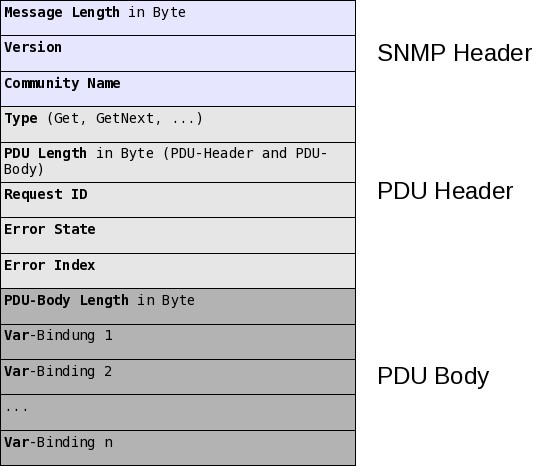
\includegraphics[width=0.8\linewidth]{images/theorie/snmp-packet}
  \caption[Aufbau eines SNMP-Pakets]{Aufbau eines SNMP-Pakets. Die in der MIB definierten Daten werden als MO, also Key-Value Paar, im PDU-Body nacheinander angegeben. Achtung: Der PDU-Header bei einem TRAP-Paket weist andere Daten auf, der PDU-Body ist jedoch gleich aufgebaut.}
  \label{fig:snmp-packet}
\end{figure}

\begin{figure}[H]
  \lstset{morecomment=[l]{--}}
  \begin{lstlisting}[label=code:mib-inetAddress,caption={[SNMP-MIB einer IPv4-Adresse]MIB-Definition f\"ur eine IP-Adresse - definiert in der INET-ADDRESS-MIB}]
InetAddressIPv4 ::= TEXTUAL-CONVENTION
    DISPLAY-HINT "1d.1d.1d.1d"
    STATUS       current
    DESCRIPTION
        "Denotes a generic Internet address...."
    SYNTAX       OCTET STRING (SIZE (4))
  \end{lstlisting}
  \label{code:mib-ipAddress}
\end{figure}


%% Code-Fragmente: Praktische Umsetzung
\begin{figure}[H]
 \lstset{language=[ISO]C++}
 \begin{lstlisting}[label=alg:praxis-basis-netservice,caption={[Datenstruktur Helper.NetService]Die Datenstruktur Helper.NetService wird verwendet um die Verf\"ugbarkeit eines Dienstes, respektive eines Monitoring-Modules, auf einem System zu definieren.}]
  public struct NetService {
    public string host;
    public string monitor;
    public string network;
    public bool available;
    public string to_string() {
      return @"host: $host\nmonitor: $monitor\nnetwork:"+
              "$network\navailable: %s".printf(available?"Yes":"No");
    }
  }

 \end{lstlisting}
\end{figure}

\begin{figure}[H]
 \lstset{language=[ISO]C++}
 \begin{lstlisting}[label=alg:praxis-basis-kernel-msg,caption={[Asynchrone MessageQueue und Datentyp RequestData]Die asynchrone Queue, typisiert auf \texttt{RequestData}, beinhaltet alle Nachrichten\index{Nachricht}, welche nacheinander abgearbeitet werden. Die Nachrichten werden durch die Klasse \texttt{RequestData} definiert, wobei das Kommando immer angegeben werden muss, die Daten sind jedoch optional.\index{MessageQueue}\index{RequestData}}]
  AsyncQueue<RequestData> request_queue;

  class RequestData {
    public string command {get; private set;}
    public string data {get; private set;}
    public RequestData(string cmd, string? args="") {
      command = cmd;
      data = args;
    }
  }
 \end{lstlisting}
\end{figure}

\begin{figure}[H]
 \lstset{language=[ISO]C++}
 \begin{lstlisting}[label=alg:praxis-basis-imainmodule,caption={[Interface: IMainModule]Das Haupt-Interface von Plugins beinhaltet nur Methoden zur Registrierung des Modul-Containers sowie Properties f\"ur den Identifier und den Pfad, welche in der Einstiegsfunktion des Plugins schon definiert sind.}]
interface IMainModule : Object {
  public abstract void setRegistrar(PluginRegistrar registrar);
  public abstract string identifier { public get; public set; }
  public abstract string path { public get; public set; }
}
 \end{lstlisting}
\end{figure}

\begin{figure}[H]
 \lstset{language=[ISO]C++}
 \begin{lstlisting}[label=alg:praxis-basis-icommodule,caption={[Interface: ICommModule]Das Interface eines Netzwerk- und BUS-Modules. Die Signale \texttt{onError}, \texttt{onData} und \texttt{onComplete} k\"onnen auf mehrere unterschiedliche Empf\"anger gebunden werden.}]
interface ICommModule : IMainModule {
  public signal void onError(string ip, string data, int code);
  public signal void onData(string ip, string data, bool more);
  public signal void onComplete(string ip, string[] data,
                                int code);

  public abstract async void send(string? data="");
  public abstract void setParam(string key, string value);
  public abstract string getParam(string key);
}
 \end{lstlisting}
\end{figure}

\begin{figure}[H]
 \lstset{language=[ISO]C++}
 \begin{lstlisting}[label=alg:praxis-basis-imonitormodule,caption={[Interface: IMonitorModule]Das Interface eines \"Uberwachungsmoduls besteht haupts\"achlich aus der Methode \texttt{monitor()}, welche asynchron definiert ist, um nicht auf eine R\"uckmeldung warten zu m\"ussen. Die Properties \texttt{timeout}, \texttt{next\_run} und \texttt{running} dienen zur Pr\"ufung, ob ein Modul aktuell eine Pr\"ufung durchf\"uhrt oder nicht, sowie um den Zeitpunkt der n\"achsten Pr\"ufung zu berechnen.}]
interface IMonitorModule : IMainModule {
  public abstract int timeout { public get; public set;
                                default=1; }
  public abstract long next_run { public get; public set;
                                  default=0; }
  public abstract bool running { public get; public set;
                                 default=false; }

  public abstract void setParam(string key, string value);
  public abstract string getParam(string key);

  public async abstract void monitor();
}
 \end{lstlisting}
\end{figure}

\begin{figure}[H]
 \lstset{language=[ISO]C++}
 \begin{lstlisting}[label=alg:praxis-basis-idatamodule,caption={[Interface: IDataModule]Das Interface eines Datenmodules beinhaltet Methoden zum Auslesen wie auch zum Schreiben von Daten. Zus\"atzlich sind noch verschiedene Datentypen, Konstanten und Strukturen definiert, welche bei der Initialisierung und der Datenbehandlung gebraucht werden. Die zus\"atzlichen Konstanten, Strukturen und Datentypen werden hier nur exemplarisch dargestellt.}]
interface IDataModule : IMainModule {
  public abstract IDataModule.DataType data_type { public get;
                                                   public set; };
  public abstract bool open(string db_name);
  public abstract bool select(string? fields="*",
                              string? groupBy="");
  public abstract void setWhere(string field, string value);
  public abstract bool hasNext();
  public abstract IDataModule.DataSet[] getCurrent();
  public abstract string getValue(string field);
  public abstract bool save(IDataModule.DataSet[] values,
                            IDataModule.DataSet[]? where=null);
  public abstract bool delete(IDataModule.DataSet[] where);
  public abstract bool empty();

  public struct DataSet { ... };
  public struct SchemaField { ... };
  public enum DataType { ... };
  public enum SchemaFieldType { ... };

  public const string TABLE_XX = "Tablename";
  public const string[] SCHEMA_XX = {
      "name,type,length,defval,primkey",
      "..."
  };
}
 \end{lstlisting}
\end{figure}

\begin{figure}[H]
 \lstset{language=[ISO]C++}
 \begin{lstlisting}[label=alg:praxis-basis-ialertmodule,caption={[Interface: IAlertModule]Das Interface eines Alert-Modules ist sehr einfach und besitzt eigentlich nur eine Methode um einen Alert zu senden, ein Signal f\"ur die \"Ubermittlungsbest\"atigung und eine Methode zur Konfiguration des Modules.}]
interface IAlertModule : IMainModule {
  public signal void onSent(string[] recp, string uid,
                            int state, string? msg="");
  public abstract void setParam(string key, string value);
  public abstract async void send(string subject,
                                  string short_message,
                                  string message,
                                  string[]? attach=null);
}
 \end{lstlisting}
\end{figure}

\begin{figure}[H]
 \lstset{language=[ISO]C++}
 \begin{lstlisting}[label=alg:praxis-basis-iremotemodule,caption={[Interface: IRemoteModule]Ein Remote-API Modul muss lediglich bei der Instanzierung konfiguriert werden. Anschliessend wird \"uber die Methode \texttt{startThread()} ein eigener Thread gestartet, welcher die komplette Kommunikation mit den Clients \"ubernimmt. Der Konformit\"at zuliebe wurde die Methode \texttt{parseRequest(string? data="`"')} dennoch in das Interface aufgenommen.}]
interface IRemoteModule : IMainModule {
  public abstract void startThread();
  public abstract void setParam(string key, string value);
  public abstract void parseRequest(string? data="");
}
 \end{lstlisting}
\end{figure}


%% Remote-System Kommunikation
\begin{table}[H]
\centering
\begin{tabular}{c|l|p{7.3cm}}
 \toprule
 Kommando & Daten & Beschreibung\\
 \midrule
 discover & \texttt{IP-ADDRESS MASK} & Startet die automatische Suche nach Systemen im angegebenen Netzwerk.\\
 \midrule
 testdata & \texttt{IP-ADDRESS MASK NUM} & Erstellt \texttt{NUM} Pseudo-Systeme in der Datenbank im angegebenen Netzwerk f\"ur verschiedene Tests.\\
 \midrule
 testdata & - & Ohne Daten werden alle Pseudo-Systeme aus der Netzwerk- und der Hosts-Tabelle entfernt, nicht jedoch aus dem Monitoring.\\
 \midrule
 monitor & \texttt{IP-ADDRESS[ ...]} & Teilt dem System mit, dass es f\"ur die \"Uberwachung aller angegebenen IP-Adressen zust\"andig ist.\\
 \midrule
 synchronize & - & Ohne Daten wird die Synchronisation gestartet.\\
 \midrule
 synchronize & \texttt{netw ($\backslash$t A.B.C.D/MASK)+} & Durch das Prefix "`netw"' sowie der Angabe aller Netzwerke als Tabulator getrennte Liste, werden alle Netzwerke aus der Datenbank durch die angegebenen ersetzt.\\
 \midrule
 synchronize & \texttt{host $\backslash$t IP ($\backslash$t MOD;KEY;VAL)+} & Durch das Prefix "`host"' sowie der Angabe einer IP-Adresse werden alle Hosts-Eintr\"age aus der Datenbank entfernt. Die Tabulator getrennte Liste, bestehend aus den Angaben "`ModuleName;Key-Name;Wert"', wird anschliessend verwendet um neue Datens\"atze zu generieren.\\
 \midrule
 alert & \texttt{MODULE IP-ADDRESS GUID} & Teilt dem System mit, dass das gegebene Modul bei dem System fehlgeschlagen und ein Alert mit der GUID versendet worden ist.\\
 \midrule
 rebuild & - & Verkn\"upft alle Systeme zu einem neuen \"Uberwachungs-Netzwerk.\\
 \midrule
 exit & - & Beendet das System.\\
 \bottomrule
\end{tabular}
\caption[Kommandos f\"ur entfernte Systeme]{Kommandos und Daten, die ein entferntes System senden kann.}
\label{tbl:praxis-basis-kernel-remote}
\end{table}


%% Datenbank-Tabellen
\begin{table}[H]
\centering
\begin{tabular}{l|c|c|l|c|p{8cm}}
 \toprule
 Feld & Typ & L\"ange & Std. & PK & Beschreibung\\
 \midrule
 section & string & 20 & - & No & Bereich des Parameter\\
 \midrule
 key & string & 50 & - & No & Parameter Name\\
 \midrule
 value & text & - & - & No & Parameter Wert\\
 \bottomrule
\end{tabular}
\caption[Datenbank-Tabelle: CONF]{Datenbank \texttt{CONF}: Konfiguration verschiedener Systembereiche.}
\label{tbl:praxis-basis-data-table_conf}
\end{table}
% SCHEMA_CONF = {"section,string,20,,0", "key,string,50,,0", "value,text,,,0"};

\begin{table}[H]
\centering
\begin{tabular}{l|c|c|l|c|p{7cm}}
 \toprule
 Feld & Typ & L\"ange & Std. & PK & Beschreibung\\
 \midrule
 network & string & 39 & - & No & Netzwerk (IP-)Adresse\\
 \midrule
 mask & int & 2 & 0 & No & Subnetmaske\\
 \midrule
 discoverable & int & 1 & 0 & No & Das Netzwerk kann untersucht werden 1=ja, 0=nein\\
 \midrule
 vpn\_gateway & string & 39 & - & No & Adresse des VPN-Gateway in dieses Netzwerk\\
 \midrule
 vpn\_user & string & 20 & - & No & Benutzer f\"ur die OpenVPN-Verbindung\\
 \midrule
 vpn\_pass & string & 20 & - & No & Passwort f\"ur die OpenVPN-Verbindung\\
 \midrule
 is\_test & int & 1 & 0 & No & Ist auf 1, wenn es sich um ein Pseudo-Test-Netzwerk handelt\\
 \bottomrule
\end{tabular}
\caption[Datenbank-Tabelle: NETWORKS]{Datenbank \texttt{NETWORKS}: Definition der verschiedenen Netzwerke, die \"uberwacht werden.}
\label{tbl:praxis-basis-data-table_netw}
\end{table}
% SCHEMA_NETWORKS = {"network,string,39,,0", "mask,int,2,0,0", "discoverable,int,1,0,0", "vpn_gateway,string,20,,0", "vpn_user,string,20,,0", "vpn_pass,string,20,,0", "is_test,int,1,0,0"};

\begin{table}[H]
\centering
\begin{tabular}{l|c|c|l|c|p{8cm}}
 \toprule
 Feld & Typ & L\"ange & Std. & PK & Beschreibung\\
 \midrule
 host & string & 39 & - & No & Adresse des zu \"uberwachenden Systems\\
 \midrule
 module & string & 20 & - & No & Modulname\\
 \midrule
 key & string & 50 & - & No & Parameter-Name\\
 \midrule
 value & text & - & - & No & Parameter-Wert\\
 \midrule
 is\_test & int & 1 & 0 & No & Ist auf 1, wenn es sich um ein Pseudo-Test-Host handelt\\
 \bottomrule
\end{tabular}
\caption[Datenbank-Tabelle: HOSTS]{Datenbank \texttt{HOSTS}: Alle Systeme und \"Uberwachngs-Dienste sowie Konfigurationsparameter, welche bei einem Host-Discovery gefunden wurden.}
\label{tbl:praxis-basis-data-table_hosts}
\end{table}
% SCHEMA_HOSTS = {"host,string,39,,0", "module,string,20,,0", "key,string,50,,0", "value,text,,,0", "is_test,int,1,0,0"};

\begin{table}[H]
\centering
\begin{tabular}{l|c|c|l|c|p{8cm}}
 \toprule
 Feld & Typ & L\"ange & Std. & PK & Beschreibung\\
 \midrule
 host & string & 39 & - & No & Adresse des zu \"uberwachenden Systems\\
 \midrule
 module & string & 20 & - & No & Modulname\\
 \midrule
 key & string & 50 & - & No & Parameter-Name\\
 \midrule
 value & text & - & - & No & Parameter-Wert\\
 \bottomrule
\end{tabular}
\caption[Datenbank-Tabelle: MODULES]{Datenbank \texttt{MODULES}: Alle Systeme und \"Uberwachungs-Dienste sowie deren Parameter.}
\label{tbl:praxis-basis-data-table_modules}
\end{table}
% SCHEMA_MODULES = {"module,string,20,,0", "host,string,39,,0", "key,string,50,,0", "value,text,,,0"};

\begin{table}[H]
\centering
\begin{tabular}{l|c|c|l|c|p{8cm}}
 \toprule
 Feld & Typ & L\"ange & Std. & PK & Beschreibung\\
 \midrule
 host & string & 39 & - & No & Adresse des zu \"uberwachenden Systems\\
 \midrule
 module & string & 20 & - & No & Modulname\\
 \midrule
 state & uint & 4 & 0 & No & Status\\
 \midrule
 time & uint & 11 & 0 & No & Timestamp\\
 \midrule
 message & text & - & - & No & Nachricht/Daten\\
 \bottomrule
\end{tabular}
\caption[Datenbank-Tabelle: MONITOR]{Datenbank \texttt{MONITOR}: Alle Monitoring-Nachrichten.}
\label{tbl:praxis-basis-data-table_monitor}
\end{table}
% SCHEMA_MONITOR = {"module,string,20,,0", "host,string,39,,0", "state,uint,4,0,0", "time,uint,11,0,0", "message,text,,,0"};

\begin{table}[H]
\centering
\begin{tabular}{l|c|c|l|c|p{7.5cm}}
 \toprule
 Feld & Typ & L\"ange & Std. & PK & Beschreibung\\
 \midrule
 host & string & 39 & - & No & Adresse des zu \"uberwachenden Systems\\
 \midrule
 module & string & 20 & - & No & Modulname\\
 \midrule
 subject & string & 20 & - & No & Betreff der Nachricht\\
 \midrule
 short & string & 160 & - & No & Kurze Meldung\\
 \midrule
 message & text & - & - & No & Ausf\"uhrliche Meldung\\
 \midrule
 uid & string & 64 & - & No & Die GUID des Alerts\\
 \bottomrule
\end{tabular}
\caption[Datenbank-Tabelle: ALERT]{Datenbank \texttt{ALERT}: Alle Alert-Nachrichten, die durch das aktuelle System versandt worden w\"aren. Es werden auch die Nachrichten gespeichert, welche aufgrund des Timeouts nicht versendet worden sind.}
\label{tbl:praxis-basis-data-table_alert}
\end{table}
% SCHEMA_ALERT = {"module,string,20,,0", "host,string,39,,0", "subject,string,20,,0", "short,string,160,,0", "message,text,,,0", "attachment,blob,,,0"};

\begin{table}[H]
\centering
\begin{tabular}{l|c|c|l|c|p{7.5cm}}
 \toprule
 Feld & Typ & L\"ange & Std. & PK & Beschreibung\\
 \midrule
 host & string & 39 & - & No & Adresse des zu \"uberwachenden Systems\\
 \midrule
 module & string & 20 & - & No & Modulname\\
 \midrule
 tstamp & uint & 11 & 0 & No & Zeitstempel des aktuellen Systems\\
 \midrule
 sent\_host & string & 39 & - & No & Adresse des Systems, welches die Nachricht versandt hat\\
 \midrule
 uid & string & 64 & - & No & Die GUID des Alerts\\
 \bottomrule
\end{tabular}
\caption[Datenbank-Tabelle: ALERT\_SENT]{Datenbank \texttt{ALERT\_SENT}: Alle Alert-Nachrichten, welche von anderen und diesem System versandt worden sind. Dient zur Pr\"ufung, ob eine Benachrichtigung versendet werden soll oder nicht.}
\label{tbl:praxis-basis-data-table_alertsent}
\end{table}
% SCHEMA_ALERT_SENT = {"module,string,20,,0", "host,string,39,,0", "tstamp,uint,11,0,0", "sent_host,string,39,,0"};

% Pseudo-Konfiguration der TechDemo
\begin{table}[H]
\centering
\begin{tabular}{l|l|p{8cm}}
 \toprule
 Key & Value & Beschreibung\\
 \midrule
 to\_list & em@il.dom,em@il.dom & Kommaseparierte Liste mit allen EMail-Adressen, an welche ein Alert versendet werden soll\\
 \midrule
 mail\_from & em@il.dom & EMail-Adresse des Alert-Absenders\\
 \midrule
 host & IP-Address | DNS & IP-Adresse oder DNS-Name des MX-Servers\\
 \midrule
 auth\_method & plain | login & Authentifizierungs-Methode. Aktuell werden LOGIN und PLAIN unterst\"utzt\\
 \midrule
 username & em@ail.com & Benutzername f\"ur Relaying\\
 \midrule
 password & abc & Passwort zum obigen Benutzernamen\\
 \bottomrule
\end{tabular}
\caption[Datei dummy\_alert\_config.txt]{Die Datei "`dummy\_alert\_config.txt"' im data-Ordner beinhaltet aktuell die Konfiguration des EMail-Alert-Modules. Key und value werden durch einen Doppelpunkt getrennt: "`host:1.2.3.4"'.}
\label{tbl:praxis-install-dummyalertconf}
\end{table}





%% Eidesstattliche Erkl\"arung
\newpage
%\addcontentsline{toc}{chapter}{Selbst\"andigkeitserkl\"arung}
\chapter*{Selbst\"andigkeitserkl\"arung}
\noindent
Ich erkl\"are hiermit, dass ich diese Thesis selbst\"andig verfasst und keine andern als die angegebenen Quellen benutzt habe. Alle Stellen, die w\"ortlich oder sinngem\"ass aus Quellen entnommen wurden, habe ich als solche kenntlich gemacht. Ich versichere zudem, dass ich bisher noch keine wissenschaftliche Arbeit mit gleichem oder \"ahnlichem Inhalt an der Fernfachhochschule Schweiz oder an einer anderen Hochschule eingereicht habe. Mir ist bekannt, dass andernfalls die Fernfachhochschule Schweiz zum Entzug des aufgrund dieser Thesis verliehenen Titels berechtigt ist.

\noindent
\newline\newline\newline\newline
\begin{tabular}{p{4.5in}}
    \hline \\
    Lommis, 09. Februar 2011
\end{tabular}

\end{document}
